\documentclass[openany,g5paper,electronic]{kthesis}

\setcounter{tocdepth}{4}
\setcounter{secnumdepth}{4}

\usepackage[T1]{fontenc}
\usepackage{textcomp}
\usepackage{lmodern}
\usepackage[latin1,utf8]{inputenc}
\usepackage[swedish, english]{babel}
\usepackage{tocloft}
\usepackage{multirow}
\usepackage{adjustbox}
\usepackage{graphicx,booktabs}
\usepackage{float}
\usepackage{rotating}
\usepackage{amsthm}
\usepackage{adjustbox}
\usepackage{varwidth} %for the varwidth minipage environment
\usepackage[listings,skins]{tcolorbox}
\usepackage{csquotes}
\usepackage{makeidx} 
\usepackage{enumitem}
%\usepackage{graphics}
%\usepackage{amssymb}
%\usepackage{amsmath}
\usepackage{graphicx}
\usepackage{caption}
\usepackage{listings}
\usepackage{newfloat}
\usepackage[cmex10]{amsmath}
\usepackage{subcaption}
\usepackage[square,numbers]{natbib}
%\usepackage{color} 
%\usepackage{transparent} 
%\usepackage{bm} % bold math
%\usepackage{fmtcount}
%\usepackage{booktabs}
\usepackage{xspace}
\usepackage{tikz}
%\usepackage{algpseudocode}
%\usepackage{algorithm}
\usepackage{algorithm2e}
\usepackage{url}
\usepackage{xurl}
%\usepackage{cite}
\PassOptionsToPackage{hyphens}{url}\usepackage{hyperref}
\usepackage[singlelinecheck=off]{caption}
\hypersetup{
    colorlinks,
    citecolor=black,
    filecolor=black,
    linkcolor=black,
    urlcolor=black
}

% FONTS
\usepackage{lmodern}
\usepackage[T1]{fontenc}
\usepackage{xifthen}% provides \isempty test
\usepackage{xcolor}
\usepackage[explicit]{titlesec}
\usepackage{titletoc}
\usepackage{pdfpages}
\usepackage{comment}
\usepackage[
    left = \flqq{},% 
    right = \frqq{},% 
    leftsub = \flq{},% 
    rightsub = \frq{} %
]{dirtytalk}

% Layout
\definecolor{bluekth}{rgb}{0.16, 0.42, 0.705}

% 0.16, 0.42, 0.705  107/255


% chapter tiltes formatting
\titleformat{\chapter}[display]
  {\LARGE}
  {\renewcommand{\thechapter}{{\color{gray}0}\arabic{chapter}\color{gray}\vspace{2.0ex}\titlerule}
  %\colorbox{blacm}
  {{\bfseries\fontsize{40}{50}\selectfont
  \thechapter\hspace*{-1.5cm}
    \parbox[t][1.2cm][t]{1cm}{%
      \centering\textcolor{black}  {}}}}}
  {-3ex}
  {%\color{black}\titlerule
  \vspace{-12.5ex}\filleft\parbox[b]{0.5\textwidth}{\begin{flushright}\MakeUppercase{#1}\\\end{flushright}}\hspace*{-0.08cm}\vspace{-0.5cm}}
  [\vspace{0.1ex}]
% chapter tiltes spacing
\titlespacing*{\chapter}{0pt}{10pt}{50pt}

% section tiltes formatting
\titleformat{\section}
  {\LARGE}{\MySecSquare\ \thesection}{1em}{#1}

\titleformat{name=\section,numberless}
  {\Large}{\MySecSquare}{1em}{#1}

% subsection tiltes formatting
\titleformat{\subsection}
  {\large}{\MySecSquare}{1em}{#1}

\titleformat{name=\subsection,numberless}
  {\large}{\hspace{0.25em}\MySecSquare\hspace{0.45em}\thesubsection}{1em}{#1}



% formatting for chapter entries in ToC  
%\titlecontents{chapter}
%  [1em]{}
%  {\tiny\thecontentslabel{2.3em}}
%  {\hspace*{-2.3em}}
%  {\hfill\contentspage}
  

% formatting for section entries in ToC  
\titlecontents{section}
  [3.0em]
  {\addvspace{3pt}}%
  {\normalsize\contentslabel{2.3em}}
  {}
  {\titlerule*[1pc]{.}\contentspage}


%\titlecontents{subsection}
%  [10.0em]
%  {\addvspace{3pt}}
%  {\normalsize\contentslabel{2.3em}}
%  {\hspace*{-2.3em}}
%  {\titlerule*[1pc]{.}\contentspage}


  
% Square to be used in itemize
\newcommand\MySquare{%
  \leavevmode\hbox to 1.2ex{\hss\vrule height .9ex width .7ex depth -.2ex\hss}}
% Square to be used in section titles
\newcommand\MySecSquare{%
  \leavevmode\hbox to 1.2ex{\hss\vrule height 1.3ex width 1.1ex depth -.2ex\hss}}


% First level of itemize uses a square
\renewcommand\labelitemi{\MySquare}

%\setcounter{tocdepth}{2}
%\setcounter{secnumdepth}{4}

%%% This is a patch for the correct numbering
\newcounter{patchino}


\newcommand{\msubsection}[1]{
  \stepcounter{patchino}
  \setcounter{subsection}{\thepatchino}
  \subsection{#1}
}


\newcommand{\msection}[1]{
  \setcounter{patchino}{0}
  \section{#1}
}

\usetikzlibrary{tikzmark,calc,decorations.pathreplacing}
\newcommand{\Depth}{2}
\newcommand{\Height}{2}
\newcommand{\Width}{2}

\renewcommand{\labelitemi}{\textcolor{IndianRed3}{\bfseries\textbullet}}


%% For autorefname
\addto\extrasenglish{%
  \renewcommand{\sectionautorefname}{Section}
  \renewcommand{\chapterautorefname}{Chapter}
  \renewcommand{\subsubsectionautorefname}{Subsection}
  \renewcommand{\subsectionautorefname}{Subsection}
  \renewcommand{\algorithmautorefname}{Algorithm}
}
\DeclareGraphicsExtensions{.pdf,.png,.jpg,.eps}

\DeclareFloatingEnvironment[fileext=frm,placement={tph},name=Listing]{code}
\captionsetup[lstlisting]{singlelinecheck=false, margin=0pt}


\newcommand{\termidx}[2][]{%
    \ifthenelse{\isempty{#1}}%
    {#2} % 
    {#1} %
    \index{#2}
  }
  \newcommand{\ie}{\textit{i.e.,}\xspace}
  \newcommand{\etal}{et al.\xspace}


\newcommand{\subscript}[2]{$#1 _ #2$}

\newcommand{\libsodiumfunctions}{869}
\newcommand{\qrcodefunctions}{1849}
\newcommand{\allmewefunctions}{\libsodiumfunctions + \qrcodefunctions}

% Execute a python script for small calculations
\newcommand{\pypy}[1]{\input{|python3 interpreter.py #1}}
\newcommand{\fromjson}[2]{\input{| jq -r '#2' '#1}}

\newcommand{\corpusrosetta}{Rosetta\xspace}
\newcommand{\corpussodium}{Libsodium\xspace}
\newcommand{\corpusqrcode}{QrCode\xspace}


\newcommand{\DTWStatic}{dt\_static\xspace}
\newcommand{\DTW}{TraceDiff\ }
\newcommand{\crow}{CROW\xspace}
\newcommand{\mewe}{MEWE\xspace}
\newcommand{\wmutate}{wasm-mutate\xspace}


\newcommand{\wasm}{Wasm\xspace}
\newcommand{\Wasm}{WebAssembly\xspace}


\usepackage{catchfile}
\newcommand{\getenv}[2][]{%
  \CatchFileEdef{\temp}{"|kpsewhich --var-value #2"}{\endlinechar=-1}%
  \if\relax\detokenize{#1}\relax\temp\else\let#1\temp\fi}




\newcommand{\wrule}[1]{
  \vspace{3mm}\noindent\textbf{#1}
}


% \renewcommand{\texttt}[1]{\lstinline{#1}}


%% TIkz probes
\newcommand\tikzmarkWS[5]{%
\tikz[remember picture, overlay]{%
        \pgfusepath{use as bounding box}%
        \node[right=#3 mm, fill=white!0, draw=black!40,text width=#5,align =center,outer sep=-0.5pt,inner xsep=1pt, inner ysep=1.5pt, rounded corners=3pt,anchor=north, minimum height=#4 mm, text depth = #4 mm] at (1 mm,2 mm) (#1) {#2};
      %\node[right=#3 mm, align=center, shape=circle,text=black,draw=black, fill=white,inner sep=0.5pt] (#1) {#2};
  }
 }
 

\newcommand\tikzmarkMap[5]{%
\tikz[remember picture, overlay]{%
        \pgfusepath{use as bounding box}%
        \node[right=#3 mm, fill opacity=0, draw opacity=0.5,text width=#5,align =center,outer sep=-0.5pt,inner xsep=1pt, inner ysep=1.5pt, rounded corners=3pt,anchor=north, minimum height=#4 mm, text depth = #4 mm] at (1 mm,2 mm) (#1) {};
      %\node[right=#3 mm, align=center, shape=circle,text=black,draw=black, fill=white,inner sep=0.5pt] (#1) {#2};
  }
 }

\newcommand\tikzmarkJS[4]{%
\tikz[remember picture, overlay]{%
        \pgfusepath{use as bounding box}%
        \node[right=#3 mm, fill=yellow!20,text width=2mm,align =center,outer sep=0pt,inner xsep=1pt, inner ysep=0pt, rounded corners=3pt,anchor=north, minimum height=#4 mm, text depth = #4 mm] at (1 mm,2 mm) (#1) {#2};
      %\node[right=#3 mm, align=center, shape=circle,text=black,draw=black, fill=white,inner sep=0.5pt] (#1) {#2};
  }
 }
 
 \newcommand\tikzmarkPROBE[4]{%
\tikz[remember picture, overlay]{%
        \pgfusepath{use as bounding box}%
        \node[right=#3 mm,text width=2mm,align =center,outer sep=0pt,inner xsep=1pt, inner ysep=0pt, rounded corners=3pt,anchor=north, minimum height=#4 mm, text depth = #4 mm] at (1 mm,2 mm) (#1) {};
      %\node[right=#3 mm, align=center, shape=circle,text=black,draw=black, fill=white,inner sep=0.5pt] (#1) {#2};
  }
 }
  
 \newcommand{\toolcite}[1]{\footnote{\url{#1}}}

 \def\checkmark{\tikz\fill[scale=0.4](0,.35) -- (.25,0) -- (1,.7) -- (.25,.15) -- cycle;} 


\newcommand*\badge[1]{ \colorbox{red}{\color{white}#1}}
\newcommand*\badget[1]{\colorbox{red}{\color{white}#1}}
\newcommand*\badgeg[1]{\colorbox{green}{\color{white}#1}}


\makeatletter
\newenvironment{btHighlight}[1][]
{\begingroup\tikzset{bt@Highlight@par/.style={#1}}\begin{lrbox}{\@tempboxa}}
{\end{lrbox}\bt@HL@box[bt@Highlight@par]{\@tempboxa}\endgroup}


\definecolor{commentgreen}{RGB}{176, 176, 176}
\definecolor{rowcolor}{cmyk}{0,0.87,0.68,0.32}
\definecolor{rowcolor2}{cmyk}{ 20, 0, 37, 34}

\definecolor{eminence}{RGB}{108,48,130}
\definecolor{weborange}{RGB}{255,165,0}
\definecolor{frenchplum}{RGB}{129,20,82}
\definecolor{darkgreen}{RGB}{10, 92, 10}


\definecolor{celadon}{rgb}{0.67, 0.88, 0.69}
%\renewcommand{\blue}{}

\newcommand\btHL[1][]{%
  \begin{btHighlight}[#1]\bgroup\aftergroup\bt@HL@endenv%
}
\def\bt@HL@endenv{%
  \end{btHighlight}%   
  \egroup
}
\newcommand{\bt@HL@box}[2][]{%
  \tikz[#1]{%
    \pgfpathrectangle{\pgfpoint{1pt}{0pt}}{\pgfpoint{\wd #2}{\ht #2}}%
    \pgfusepath{use as bounding box}%
    \node[anchor=base west, fill=orange!30,outer sep=0pt,inner xsep=1pt, inner ysep=0pt, rounded corners=3pt, minimum height=\ht\strutbox+1pt,#1]{\raisebox{1pt}{\strut}\strut\usebox{#2}};
  }%
}
\makeatother

\makeatletter


\lstdefinelanguage{C}{
    otherkeywords={},
    morekeywords=[1]{const, int},
    morekeywords=[2]{0},
    morekeywords=[3]{add,const,mul,shl,get,rem_s,rem_u,ne,tee,sub,set,store},
    morekeywords=[4]{},
    morekeywords=[5]{global, get_global, mut, set_global, export, import,loop, memory, data, get_local,if, block,module, set_local,call,br_if,end, all,call_indirect,local,global,module, func, param, result, type},
    morekeywords=[6]{=,;},
    morekeywords=[7]{(,),[,],.},
    sensitive=false,
    morecomment=[l]{;},
    morecomment=[s]{;}{;},
    morestring=[b]",
    keywordstyle=[1]\color{eminence}\bfseries,
    keywordstyle=[3]\color{frenchplum},
    keywordstyle=[5]\color{darkgreen}\bfseries,
    commentstyle=\color{commentgreen}
}

\lstdefinelanguage{WAT}{
    otherkeywords={},
    morekeywords=[1]{i32,f32,i64,f64},
    morekeywords=[2]{0},
    morekeywords=[3]{add,const,mul,shl,get,rem_s,rem_u,ne,tee,sub,set,store},
    morekeywords=[4]{},
    morekeywords=[5]{global, get_global, mut, set_global, export, import,loop, memory, data, get_local,if, block,module, set_local,call,br_if,end, all,call_indirect,local,global,module, func, param, result, type},
    morekeywords=[6]{=,;},
    morekeywords=[7]{(,),[,],.},
    sensitive=false,
    morecomment=[l]{;},
    morecomment=[s]{;}{;},
    morestring=[b]",
    keywordstyle=[1]\color{eminence}\bfseries,
    keywordstyle=[3]\color{frenchplum},
    keywordstyle=[5]\color{darkgreen}\bfseries,
    commentstyle=\color{commentgreen}
}
\lstdefinelanguage{llvm}{
    morecomment = [l]{;},
    morestring=[b]", 
    sensitive = true,
    morekeywords=[2]{i32,f32,i64,f64},
    morekeywords=[3]{
        define, declare, global, constant,
        internal, external, private,
        linkonce, linkonce_odr, weak, weak_odr, appending,
        common, extern_weak,
        thread_local, dllimport, dllexport,
        hidden, protected, default,
        except, deplibs,
        volatile, fastcc, coldcc, cc, ccc,
        x86_stdcallcc, x86_fastcallcc,
        ptx_kernel, ptx_device,
        signext, zeroext, inreg, sret, nounwind, noreturn,
        nocapture, byval, nest, readnone, readonly, noalias, uwtable,
        inlinehint, noinline, alwaysinline, optsize, ssp, sspreq,
        noredzone, noimplicitfloat, naked, alignstack,
        module, asm, align, tail, to,
        addrspace, section, alias, sideeffect, c, gc,
        target, datalayout, triple,
        blockaddress
    },
    morekeywords=[4]{
        fadd, sub, fsub, mul, fmul,
        sdiv, udiv, fdiv, srem, urem, frem,
        and, or, xor,
        icmp, fcmp,
        eq, ne, ugt, uge, ult, ule, sgt, sge, slt, sle,
        oeq, ogt, oge, olt, ole, one, ord, ueq, ugt, uge,
        ult, ule, une, uno,
        nuw, nsw, exact, inbounds,
        phi, call, select, shl, lshr, ashr, va_arg,
        trunc, zext, sext,
        fptrunc, fpext, fptoui, fptosi, uitofp, sitofp,
        ptrtoint, inttoptr, bitcast,
        ret, br, indirectbr, switch, invoke, unwind, unreachable,
        malloc, alloca, free, load, store, getelementptr,
        extractelement, insertelement, shufflevector,
        extractvalue, insertvalue,
    },
    alsoletter={\%},
    keywordsprefix={\%},% All identifiers starting with '%' will be printed as first order keywords.
    keywordstyle=[1]\bfseries,% As mentioned above, these are the keywords starting with '%', like '%5'
    keywordstyle=[2]\color{eminence}\bfseries,
    keywordstyle=[3]\color{darkgreen}\bfseries,
    keywordstyle=[4]\color{frenchplum},
}
\makeatother

\newcommand{\todo}[1]{%
%\refstepcounter{todo}
\noindent\textbf{\badge{TODO}} {\color{red} #1}
%\addcontentsline{td}{todo}
%{\color{red}\thesection.\thetodo\xspace #1}
}

\newcommand{\done}[1]{%
\noindent\textbf{\badgeg{DONE}} {\color{green}#1}
}
\newcommand{\citationneeded}{
  \badget{[?]}
}

\newcommand*\step[1]{
\noindent\tikz[baseline=(char.base)]{
        \node[shape=circle,text=black,draw=black, fill=white,inner sep=1.2pt] (char) {#1};}}



\newtheorem{definition}{Definition}
\providecommand*{\definitionautorefname}{Definition}
\newtheorem{metric}{Metric}
\providecommand*{\metricautorefname}{Metric}



\newtheorem{property}{Property}
\providecommand*{\propertyautorefname}{Property}

\hyphenation{Web-Assembly}
\hyphenation{super-optimizers}
\hyphenation{super-optimize}

%\addcontentsline{td}{todo}
%{\color{red}\thesection.\thetodo\xspace Citation needed}}


\makeatletter
\lstset{
    %language=C,
    basicstyle=\ttfamily\footnotesize\lst@ifdisplaystyle\scriptsize\fi,
    escapeinside={\%*}{*)},
    captionpos=t
}
\makeatother


\lstdefinestyle{CStyle}{
  %numbers=none,
  stepnumber=1,
  numbersep=10pt,
  tabsize=4,
  showspaces=false,
  showstringspaces=false,
  basicstyle=\scriptsize\ttfamily,
  %moredelim=**[is][{\btHL[fill=black!10]}]{`}{`},
  moredelim=**[is][{\btHL[fill=celadon!40]}]{@}{@}
}

\lstdefinestyle{WATStyle}{
  numbers=left,
  stepnumber=1,
  numbersep=5pt,
  tabsize=4,
  showspaces=false,
  showstringspaces=false,
}

\lstdefinestyle{LLVMStyle}{
  numbers=none,
  stepnumber=0,
  numbersep=10pt,
  tabsize=4,
  showspaces=false,
  showstringspaces=true,
}



\getenv[\NOWIDOW]{NOWIDOW}
\ifthenelse{\equal{\NOWIDOW}{True}}%
    {
      \widowpenalties 1 10000
      \raggedbottom

      \setlength{\parskip}{20pt}

      \titlecontents{chapter}[0pc]
      {\addvspace{15pt}}%
      {\large\bfseries}
      {\large\bfseries}
      {\bfseries\hfill\large}%
      
      \titlecontents{subsection}
      [10.0em]{}
      {\normalsize\contentslabel{3.3em}}
      {\hspace*{-2.3em}}
      {\titlerule*[1pc]{ }}

      \titlecontents{section}
      [10.0em]{}
      {\normalsize\contentslabel{3.3em}}
      {\hspace*{-2.3em}}
      {\titlerule*[1pc]{ }}


      \renewcommand\labelitemi{}


        % section tiltes formatting
        \titleformat{\section}
        {\Large}{}{1em}{#1}
        \titleformat{name=\section,numberless}
        {\Large}{}{1em}{#1}

        % subsection tiltes formatting
        \titleformat{\subsection}
        {\Large}{}{1em}{#1}
        \titleformat{name=\subsection,numberless}
        {\Large}{}{1em}{#1}

        \titleformat{\chapter}[display]
        {\LARGE}
        {\renewcommand{\thechapter}{}
        %\colorbox{blacm}
        {{\bfseries\fontsize{30}{40}\selectfont
        \thechapter
          \parbox[c][1.2cm][c]{1cm}{%
            \centering\textcolor{black}  {}}}}}
        {-1ex}
        {%\color{black}\titlerule
        \vspace{-1.9ex}\filleft\MakeUppercase{#1}}
        [
        ]
    } % 
    {} %

%%%%%%%%%%%%%%%%%%%%%%%%%%%%%%%%%%%%%%%
%%%%%%%%% Document starts here %%%%%%%%
%%%%%%%%%%%%%%%%%%%%%%%%%%%%%%%%%%%%%%%
\begin{document}

%%%%%%%%%%%%%%%%%%%%%%%%%%%%%%%%%%%%%%%%%%
%%%%%% First and second pages %%%%%%%%%%%%
%%%%%%%%%%%%%%%%%%%%%%%%%%%%%%%%%%%%%%%%%%

%\title{Runtime randomization and perturbation for virtual machines.}
\title{ Artificial Software Diversification for WebAssembly }
\subtitle{\textbf{sub-title}}
\author{Javier Cabrera-Arteaga}
\date{date}
\thesistype{Doctoral Thesis}
\imprint{Stockholm, Sweden, 2020}
\examen{Teknologie doktorexamen i elektroteknik}
\disputationsdatum{fredagen den 18 januari 2020 klockan 14.00}
\disputationslokal{Sal F3, Lindstedtsvägen 26, Kungliga Tekniska H\"{o}gskolan, Stockholm}
\publisher{Universitetsservice US AB}
\address{KTH Royal Institute of Technology \\School of Electrical Engineering and Computer Science\\ Division of Fusion Plasma Physics \\ SE-10044 Stockholm\\ Sweden}
\isbn{ISBN 100-}
%\issn{ISSN XXX} % No longer used at KTH
\trita{TRITA-EECS-AVL-2020:4}
\kthlogo{KTHLogo}

\pretolerance=10000
\tolerance=4000 
\emergencystretch=10pt
% Create title page using info above
\maketitle

\frontmatter % Pages i, ii, iii, iv, v etc.
%%%%%%%%%%%%%%%%%%%%%%%%%%%%%%%%%%%
%%%%%%%%%%% ABSTRACT %%%%%%%%%%%%%%
%%%%%%%%%%%%%%%%%%%%%%%%%%%%%%%%%%%
\begin{abstract}
\noindent \lipsum[1]

\end{abstract}

\bigskip \bigskip \bigskip \bigskip \bigskip

\setlength{\leftskip}{0.3 cm} \textbf {Keywords:} Lorem, Ipsum, Dolor, Sit, Amet

%%%%%%%%%%%%%%%%%%%%%%%%%%%%%%%%%%%%%%%%
%%%%%%%% SWEDISH ABSTRACT %%%%%%%%%%%%%%
%%%%%%%%%%%%%%%%%%%%%%%%%%%%%%%%%%%%%%%%
\newpage
\selectlanguage{swedish}
\begin{abstract}
\noindent \lipsum[1]
\end{abstract}
\selectlanguage{english}


%%%%%%%%%%%%%%%%%%%%%%%%%%%%%%%%%%%%%%%
%%%%%%% List of papers %%%%%%%%%%%%%%%%
%%%%%%%%%%%%%%%%%%%%%%%%%%%%%%%%%%%%%%%
\chapter{List of Papers}

%\let\thefootnote\relax\footnote{Paper I and III are published under license in \textit{Journal of X}}
\vspace{1cm}
\begin{enumerate}[I]
    \item \textbf{\textit{WebAssembly Diversification for Malware Evasion}} \\
        \textbf{Javier Cabrera-Arteaga},Tim Toady, Martin Monperrus, Benoit Baudry\\
        \textit{Computers \& Security, Volume 131, 2023, 17 pages} \\
        \url{https://www.sciencedirect.com/science/article/pii/S0167404823002067}
    \item \textbf{\textit{Wasm-mutate: Fast and Effective Binary Diversification for
    WebAssembly}} \\
        \textbf{Javier Cabrera-Arteaga}, Nicholas Fitzgerald, Martin Monperrus, Benoit Baudry\\
        \textit{Under review, 17 pages} \\
        \url{https://arxiv.org/pdf/2309.07638.pdf}    
    \item \textbf{\textit{Multi-Variant Execution at the Edge}} \\
    \textbf{Javier Cabrera-Arteaga},Pierre Laperdrix, Martin Monperrus, Benoit Baudry\\
    \textit{Moving Target Defense (MTD 2022), 12 pages} \\
    \url{https://dl.acm.org/doi/abs/10.1145/3560828.3564007}

    \item \textbf{\textit{CROW: Code Diversification for WebAssembly}} \\
        \textbf{Javier Cabrera-Arteaga}, Orestis Floros, Oscar Vera-Pérez, Benoit Baudry, Martin Monperrus\\
        \textit{ Measurements, Attacks, and Defenses for the Web (MADWeb 2021), 12 pages} \\
        \url{https://doi.org/10.14722/madweb.2021.23004}
    
	\item \textbf{\textit{Superoptimization of WebAssembly Bytecode}} \\
    \textbf{Javier Cabrera-Arteaga},Shrinish Donde, Jian Gu, Orestis Floros, Lucas Satabin, Benoit Baudry, Martin Monperrus\\
    \textit{Conference Companion of the 4th International Conference on Art, Science, and Engineering of Programming (Programming 2021), MoreVMs, 4 pages} \\
    \url{https://doi.org/10.1145/3397537.3397567}
    \item \textbf{\textit{Scalable Comparison of JavaScript V8 Bytecode Traces}} \\
        \textbf{Javier Cabrera-Arteaga},Martin Monperrus, Benoit Baudry\\
        \textit{11th ACM SIGPLAN International Workshop on Virtual Machines and Intermediate Languages (SPLASH 2019), 10 pages} \\
        \url{https://doi.org/10.1145/3358504.3361228}
\end{enumerate}

%\pagebreak

%%%%%%%%%%%%%%%%%%%%%%%% Papers NOT included in THESIS
%Other contributions by the author not included in the thesis.
%\begin{enumerate}[I]%
%	\setcounter{enumi}{1}
%	\item \textbf{\textit{Title of paper}} \\
%		\textbf{First author}, Second author \\
%		\textit{Journal (year)}
%\end{enumerate}


%%%%%%%%%%%%%%%%%%%%%%%%%%%%%%%%%%%%%%%
%%%%%%%% ACKNOWLEDGMENT %%%%%%%%%%%%%%%
%%%%%%%%%%%%%%%%%%%%%%%%%%%%%%%%%%%%%%%
\chapter{Acknowledgement}

\todo{W} \todo{O}

\todo{Jury}

\todo{C}

\todo{F}

%%%%%%%%%%%%%%%%%%%%%%%%%%%%%%%%
%%%%%%%% ACRONYMS %%%%%%%%%%%%%%
%%%%%%%%%%%%%%%%%%%%%%%%%%%%%%%%
\chapter{Acronyms}
List of commonly used acronyms: \\

\begin{tabular}{llll}
\textbf{AE}		&	Acronym examples \\

\end{tabular}

%\input{Content/Dedication}\clearpage

\mainmatter % Pages 1, 2, 3...
%%%%%%%%%%%%%%%%%%%%%%%%%%%%%%%%%%%%%%
%%%%%% TABLE OF CONTENTS %%%%%%%%%%%%%
%%%%%%%%%%%%%%%%%%%%%%%%%%%%%%%%%%%%%%
\tableofcontents
\part{Thesis}
\clearpage


%%%%%%%%%%%%%%%%%%%%%%%%%%%%%%%%%%%%%%%%%%%%%%%%%%%%%%
%%%%%%%%%%%%% CHAPTER 1: INTRODUCTION %%%%%%%%%%%%%%%%
%%%%%%%%%%%%%%%%%%%%%%%%%%%%%%%%%%%%%%%%%%%%%%%%%%%%%%
\chapter{Introduction}
\label{Intro}

\chapterprecishere{Jealous stepmother and sisters; magical aid by a beast; a marriage won by gifts magically provided; a bird revealing a secret; a recognition by aid of a ring; or show; or what not; a dénouement of punishment; a happy marriage - all those things, which in sequence, make up Cinderella, may and do occur in an incalculable number of other combinations.\par\raggedleft--- {\small\textup{MR. Cox} \textbf{1893}, Cinderella: Three hundred and forty-five variants \cite{cox1893cinderella}}}


\lettrine[lines=3]{T}{he} first web browser, Nexus, made its appearance in 1990 \cite{nexus}.  
At its inception, web browsing consisted solely of retrieving and displaying small, static text pages. 
With Nexus, users could access for the first time interlinked hypertext documents, so-called HTML pages. 
However, the escalating computing power of devices, the proliferation of the internet, the valuation of internet-based companies, and the demand for more engaging user experiences gave rise the concept of executing code in conjunction with web pages. 
In 1995, the Netscape browser revolutionized this concept by introducing JavaScript \cite{10.1007/978-3-642-14107-2_7}, a programming language that allowed code execution on the client-side.
Interactive web content immediately highlighted benefits: unlike classical native software, web applications do not require installation, are always up-to-date, and are accessible from any device with a web browser. 
Significantly, since the advent of Netscape, all browsers offer JavaScript support. 
In the present day, the majority of web pages incorporate not only HTML but also JavaScript code, which is executed on client computers. 
Consequently, over the past several decades, web browsers have evolved into intricate systems capable of running comprehensive applications, such as video and audio players, animation creators, and PDF document renderers.


Despite being the main scripting language in modern web browsers, JavaScript possesses inherent limitations due to its unique language characteristics \cite{mulazzani2013fast}.
Each JavaScript engine requires the parsing and recompiling of the JavaScript code, thereby causing substantial overhead.
In practice, the process of parsing and compiling JavaScript code constitutes the majority of website load times \toolcite{https://hacks.mozilla.org/2017/02/what-makes-webassembly-fast}.
Additionally, JavaScript presents security issues, including the lack of memory isolation, which potentially enables information extraction from other processes \cite{10.1145/1190216.1190252, 10.1145/3412841.3442001}.
Numerous attempts have been made to port other languages, offering different guarantees, to the browser execution as alternatives to JavaScript.
For instance, Java applets emerged on web pages in the late 90s, enabling the execution of Java bytecode on the client side \toolcite{https://www.oracle.com/java/technologies/javase/9-deprecated-features.html}.
Likewise, Microsoft attempted twice with ActiveX in 1996 \toolcite{https://web.archive.org/web/20090828024117/http://www.microsoft.com/presspass/press/1996/mar96/activxpr.mspx}, and Silverlight in 2007 \toolcite{https://www.microsoft.com/silverlight/}.
However, these attempts either failed to persist or experienced low adoption, primarily due to security issues and the absence of consensus among the community of browser vendors.

 


Importantly, in 2014, Alon Zakai and colleagues proposed the Emscripten tool \toolcite{https://emscripten.org/}.
Emscripten employs a strict subset of JavaScript, asm.js, to facilitate the compilation of low-level code such as C to JavaScript.
Asm.js was included as an LLVM backend \toolcite{http://asmjs.org/spec/latest/}.
This strategy offered the advantages of the ahead-of-time optimizations from LLVM, resulting in performance gains on browser clients \toolcite{ttps://hacks.mozilla.org/2015/03/asm-speedups-everywhere/} when compared to standard JavaScript code.
Asm.js outperformed JavaScript because it restricted language features to those that could be optimized in the LLVM pipeline. 
Moreover, it eliminated most of the language's dynamic characteristics, limiting it to numerical types, top-level functions, and one large array in memory accessed directly as raw data.
Asm.js proved that client-side code could be enhanced with the appropriate language design and standardization.
In response to persistent JavaScript-related issues, the formalization and creation of a formal specification following asm.js laid the groundwork for the emergence of WebAssembly.
In 2015, the Web Consortium (W3C) standardized WebAssembly as a bytecode for the web environment.
As a result, WebAssembly bytecode became the fourth official language for the web.


The first distinction from earlier attempts to port non-JavaScript languages to the web lies in \Wasm's initial design. 
Unlike its predecessors, \Wasm was crafted to supplement JavaScript in the browser as a platform-agnostic, low-level bytecode, rather than to completely replace it. 
Its primary goal was to replace computing-intensive JavaScript code in contemporary web applications. 
Additionally, WebAssembly is the inaugural major language that utilized formal specification and verification right from the design inception \cite{Haas_2017, watt2018mechanising}. 


Importantly, \Wasm provides a platform for compiling several legacy code applications, like those written in C/C++. 
For example, LLVM includes \Wasm  as a backend since release 7.1.0 published in May 2019\toolcite{https://github.com/llvm/llvm-project/releases/tag/llvmorg-7.1.0}.
Therefore, the emergence of \Wasm, a fast, low-level, portable bytecode for browsers, has the potential to transform web software as we know it. 
It paves the way for web applications to undertake roles traditionally reserved for native desktop applications.
For example, applications such as AutoCAD and Adobe Photoshop have been ported to \Wasm \footnote{\url{https://twitter.com/Adobe/status/1453034805004685313?s=20&t=Zf1N7-WmzecA0K4V8R69lw}}. 


The \Wasm specification embodies several language design principles that pave the way for its extension beyond the web ecosystem.
For instance, the architecture of \Wasm guarantees self-containment.
Inherently, \Wasm binaries are prohibited from accessing memory beyond their own designated space, thereby amplifying security via Software Fault Isolation (SFI)  policies \cite{10.1145/3498688}.
Consequently, research has highlighted the benefits of integrating WebAssembly as an intermediate layer in contemporary cloud platforms \cite{pMendkiServerless}.
In particular, the employment of \Wasm binaries improves startup times and optimizes memory consumption, outperforming virtualization and containerization \cite{1244493Jacobsson}.
Furthermore, compared to virtual machines and containers, \Wasm programs are more compact, highlighting their efficient deployment, especially when network transportation is a consideration.
The methodology for standalone \Wasm execution was formalized in 2019 when the Bytecode Alliance proposed the WebAssembly System Interface (WASI) \toolcite{https://github.com/WebAssembly/WASI}.
WASI standardizes the execution of \Wasm via a POSIX-like interface protocol, thereby facilitating the execution of \Wasm closer operating system.
This standardization enables \Wasm to function outside web browsers, extending its use to cloud environments and IoT devices.

The extensive applicability and rapid adoption of \Wasm have prompted requests for additional features. 
However, these demands do not always align with the initial specifications. 
For a proposal to reach standard status, it must satisfy particular criteria.
A new proposal needs a formal specification and a minimum of two independent implementations, e.g., two different \Wasm engines. 
This approach allows for swift incorporation of new formalizations and features via the so-called "evergreen method", while maintaining the original \Wasm specification intact. 
Since the inception of \Wasm, numerous extensions have been proposed for standardization. 
For instance, the SIMD proposal enables the execution of vectorized instructions in \Wasm. 
After approval, new extensions remain optional, ensuring that the core \Wasm version remains 1.0. 
The ongoing development of \Wasm provides avenues for research and development. 
However, it also gives rise to security concerns within the ecosystem, as new threats emerge.


\msection{Predictability in \Wasm ecosystems}
Over the past three decades, web browsers and JavaScript have significant evolution, leading to myriad implementations. 
However, only Firefox, Chrome, Safari, and Edge are typically utilized on devices. 
Web page resources, including those containing WebAssembly binaries, are primarily served from centralized datacenters \cite{STRAC}. 
This situation creates a highly predictable ecosystem, where potential attackers can predict ecosystem behavior, from the browser to the code it executes. 
This predictability may be exploited to launch large-scale attacks, as predictability inherently increases the chances of successful attacks \cite{MTDNationalCyberLaep}. 
For example, if one-quarter of all devices operate the same code in the same browser, a single flaw could impact millions of devices simultaneously \cite{goth2003addressing}. 
This issue is magnified when considering the adoption of \Wasm by edge-cloud computing platforms to provide services. 
In addition to browser clients, thousands of edge devices operate millions of identical \Wasm instantiations per second. 
This suggests that if one \Wasm binary in an edge network is vulnerable, every node would be identically vulnerable due to the binary replication on each node. 
A potential attacker could compromise all edge nodes concurrently, implying that a single distributed \Wasm binary could trigger a global attack \toolcite{https://www.fastly.com/blog/defense-in-depth-stopping-a-wasm-compiler-bug-before-it-became-a-problem}.
 



% Because both malware detection and side channel attacks depends on knowing in adva'ce the behavior of your target

In the context of \Wasm, we devise two scenarios where predictability is crucial.
First, the predictability of execution ecosystems and \Wasm binaries themselves facilitates side-channel and memory attacks.
Despite the praise for WebAssembly's security, particularly its design that prohibits programs from accessing data beyond their own memory, it is not immune to such vulnerabilities. 
For example, Rokicki \etal highlighted the potential risk of port contention side-channel attacks using \Wasm malware in browsers \cite{10.1145/3488932.3517411}. 
In such cases, mitigations often involve hardware and operating-level changes, which are not always feasible.
Moreover, attacks within the memory of WebAssembly itself are feasible\cite{usenixWasm2020} as innate vulnerabilities can exist in WebAssembly binaries due to flaws in the source code. 
Besides, the lack of stack-smashing protections could result in unnoticed overflows and crashes during \Wasm executions\cite{DeRoover2022}. 
In standalone deployments, Genkin \etal demonstrated the possibility of data extraction via cache-timing side channels in \Wasm \cite{Genkin2018DrivebyKC}. 
In a similar vein, Maisuradze and Rossow exhibited speculative execution attacks on \Wasm binaries \cite{ret2spec}.


Secondly, the defenses for identifying and addressing vulnerabilities are generally predictable. 
In particular, this predictability can be manipulated by malicious actors to create programs aimed at deceiving these defense mechanisms. 
Importantly, malware can also be distributed via \Wasm binaries. 
For instance, the capability of \Wasm for efficient computation makes it an appealing target for misuse by cybercriminals, especially for cryptojacking \cite{10.1145/3339252.3339261}. 
The challenge in identifying and eliminating cryptojacking enables it to function persistently on a victim's computer, constantly utilizing resources and generating income for the attacker \cite{9566204}.  
Several techniques, such as static analysis, dynamic analysis, and even sophisticated machine learning methods, are applied to detect \Wasm malware \cite{Minesweeper,MinerRay,MINOS,SEISMIC,RAPID,Outguard}. 
However, most of these research works do not consider the predictability of an attacker knowing that a \Wasm program is not treated as obfuscated.





\msection{Problems statements}

To sum up, predictability and potential vulnerabilities form a harmful combination. 
This principle does not exclude \Wasm and its ecosystem.
The effect of exploiting a single vulnerability in \Wasm could prove catastrophic, given all devices running \Wasm binaries could be affected. 
Conversely, \Wasm malware pose a severe threat. 
Present defenses may not adequately protect against them, as they have not been designed to manage situations outside of predictable scenarios, such as obfuscation. 
Besides, mitigations might require hardware and operating-level changes, which are not always feasible.
In this dissertation, we tackle the subsequent two problems:

\begin{enumerate}[label=\textbf{P\arabic*}, ref=\textbf{P\arabic*}]

	\item \label{prob4} \textbf{Side-channels and persisting vulnerabilities}: The \Wasm ecosystem and binaries are susceptible to attacks, especially those from side-channel threats.
	
	\item \label{prob5} \textbf{\Wasm malware}: 
	\Wasm malware presents a substantial threat.
	Predictability leads to the assumption that malware is typically considered unique.

\end{enumerate}


\begin{comment}
\msection{Problem statement}

\end{comment}

\msection{Software Diversification}

This dissertation introduces tools, strategies, and methodologies designed to address the previously enunciated problem statements via Software Diversification.
Software Diversification is a security-focused process that involves identifying, developing, and deploying program variants of a given original program \cite{okhravi2013survey}.
Pioneers in this field, Cohen \etal \cite{cohen1993operating} and Forrest \etal \cite{595185}, proposed enhancing software diversity through code transformations. 
Their proposal suggested creating different and unpredictable program variants, while maintaining their functionalities, to mitigate potential vulnerabilities.



Studies have demonstrated that software diversification effectively removes vulnerabilities. 
Eichin \etal, in their seminal work of 1989, underscored the practical benefits of diversification \cite{36307}. 
They illustrated how diversification limited the exploitation of the Morris Worm to a few machines. 
From an attacker's perspective, the diversity of target systems rendered them unpredictable.
Additionally, software diversification could bolster \Wasm analysis tools by integrating diversified program variants, thereby making it harder for attackers to exploit vulnerabilities, addressing \ref{prob4}. 
On the other hand, by proactively creating variants for security purposes, a broad range of real-world conditions can be emulated, enhancing the precision of \Wasm analysis tools, including \Wasm malware detectors. 
Furthermore, it could increase the accuracy of \Wasm malware detectors and \Wasm analysis tools in general, addressing \ref{prob5}. 
Besides, the diversification process could completely disable malware from one variant to the next by removing malicious code from the original program, addressing both \ref{prob4} and \ref{prob5}. 
However, despite the extensive research, the implementation of software diversification in \Wasm is still largely unexplored. 
In light of this, we offer the following contributions within the context of software diversification, which are not necessarily mutually exclusive.


\begin{enumerate}[label=\textbf{C\arabic*}, ref=C\arabic*]

	\item \label{defensivecontrib} \wrule{Defensive Diversification:} In order to address \ref{prob4}, we assess how generated \Wasm program variants could be used for defensive purposes. We provide empirical insights about the practical usage of the generated variants in preventing attacks.
	
	\item \label{ofensivecontrib} \wrule{Offensive Diversification:} 
	In order to address \ref{prob5}, we evaluate the potential for using generated \Wasm program variants for offensive purposes. 
	Our research includes experiments where we test the resilience of \Wasm analysis tools against these generated variants. 
	Furthermore, we offer insights into which types of program variants practitioners should prioritize to improve \Wasm analysis tools.

	\item \label{methodcontrib} \wrule{Experimental contribution:} For each proposed technique we provide an artifact implementation and conduct experiments to assess its capabilities. The artifacts are publicly available. The protocols and results of assessing the artifacts provide guidance for future research on \ref{prob4} and \ref{prob5}.
	
	\item \label{therycontrib} \wrule{Theoretical contribution:} We propose a theoretical foundation in order to generate and improve Software Diversification for \Wasm. We provide a formal definition of \Wasm program variants and their diversity. We also provide a formal definition of \Wasm program diversity generation.
	
	\item \label{generationcontrib} \wrule{Diversity generation:} We generate \Wasm program variants. The variants are functionally equivalent to the original program, yet behaviorally diverse.
	

	
\end{enumerate}

\begin{table}
	\centering
	\begin{tabular}{l | c c c c }
		\multicolumn{1}{c|}{Contribution} & \multicolumn{4}{c}{Research papers} 
		\\
		&  \ref{crowpaper} & \ref{mewepaper} & \ref{wasmmutatepaper} & \ref{evasionpaper} \\
		&  \cite{CROW} & \cite{MEWE} & \cite{wasmmutate} & \cite{EVASION} \\
		\hline

		\ref{defensivecontrib} Defensive diversification   & \checkmark & \checkmark & \checkmark\\
		\ref{ofensivecontrib} Offensive diversification  & & & & \checkmark\\

		\ref{methodcontrib} Experimental contribution & \checkmark & \checkmark & \checkmark & \checkmark \\
		\ref{therycontrib} Theoretical contribution  & \checkmark &  &  \checkmark &  \\
		\ref{generationcontrib} Diversity generation   & \checkmark & \checkmark & \checkmark & \checkmark\\
	\end{tabular}
	\caption{Mapping between contributions and research papers \label{contrib_map}.}
	
\end{table}

\section{Summary of research papers}

This compilation thesis comprises the following research papers.
In \autoref{contrib_map} we map the contributions to our research papers.

\begin{enumerate}[label={\textbf{\Roman*}:}, ref={\Roman*}]
	\item \label{crowpaper} \textbf{CROW: Code randomization for WebAssembly bytecode.} \\ 
	\textbf{Javier Cabrera-Arteaga}, Orestis Floros, Oscar Vera-Pérez, Benoit Baudry, Martin Monperrus\\
	\textit{ Measurements, Attacks, and Defenses for the Web (MADWeb 2021), 12 pages} \\
	\url{https://doi.org/10.14722/madweb.2021.23004} \\
	
	\wrule{Summary:} In this paper, we introduce the first entirely automated workflow for diversifying WebAssembly binaries. 
	We present CROW, an open-source tool that implements software diversification through enumerative synthesis. 
	We assess the capabilities of CROW and examine its application on real-world, security-sensitive programs.
	In general, CROW can create many statically diverse variants. 
	Furthermore, we illustrate that the generated variants exhibit different behaviors at runtime.

	
	
	\item \label{mewepaper} \textbf{Multivariant execution at the Edge. } \\
	\textbf{Javier Cabrera-Arteaga}, Pierre Laperdrix, Martin Monperrus, Benoit Baudry\\
    \textit{Moving Target Defense (MTD 2022), 12 pages} \\
    \url{https://dl.acm.org/doi/abs/10.1145/3560828.3564007} \\

	\wrule{Summary:} 
	In this paper, we synthesize functionally equivalent variants of deployed edge services. 
	Service variants are encapsulated into a single multivariant WebAssembly binary. 
	A random variant is selected and executed each time a function is invoked.
	Execution of multivariant binaries occurs on the global edge platform provided by Fastly, as part of a research collaboration. 
	We demonstrate that multivariant binaries present a diverse range of execution traces throughout the entire edge platform, distributed worldwide, effectively creating a moving target defense.

	
	\item \label{wasmmutatepaper}\textbf{Wasm-mutate: Fast and efficient software diversification for WebAssembly. }\\ 
	\textbf{Javier Cabrera-Arteaga}, Nicholas Fitzgerald, Martin Monperrus, Benoit Baudry\\
	\textit{Submitted to Computers \& Security, 17 pages} \\
	\url{https://arxiv.org/pdf/2309.07638.pdf}

	\wrule{Summary:}
	This paper introduces WASM-MUTATE, a compiler-agnostic WebAssembly diversification engine. 
	The engine is designed to swiftly generate functionally equivalent yet behaviorally diverse WebAssembly variants by randomly traversing e-graphs. 
	We show that WASM-MUTATE can generate tens of thousands of unique WebAssembly variants in minutes. 
	Importantly, WASM-MUTATE can safeguard WebAssembly binaries from timing side-channel attacks, such as Spectre.



	\item \label{evasionpaper} \textbf{WebAssembly Diversification for Malware evasion.} \\ 
	\textbf{Javier Cabrera-Arteaga}, Tim Toady, Martin Monperrus, Benoit Baudry\\
	\textit{Computers \& Security, Volume 131, 2023, 17 pages} \\

	\wrule{Summary:}  \Wasm, while enhancing rich applications in browsers, also proves efficient in developing cryptojacking malware. 
	Protective measures against cryptomalware have not factored in the potential use of evasion techniques by attackers. 
	This paper delves into the potential of automatic binary diversification in aiming WebAssembly cryptojacking detectors' evasion. 
	We provide proof that our diversification tools can generate variants of WebAssembly cryptojacking that successfully evade VirusTotal and MINOS. 
	We further demonstrate that these generated variants introduce minimal performance overhead, thus verifying binary diversification as an effective evasion technique.

\end{enumerate}


%\todo{End up with the diagram locating our contributions in the landscape.}

\section*{Thesis layout}
This dissertation comprises two parts as a compilation thesis. 
Part one summarises the research papers included within, which is partially rooted in the author's licentiate thesis \cite{Lic}. 
Chapter 2 offers a background on \Wasm and the latest advancements in Software Diversification.  
Chapter 3 delves into our technical contributions. 
Chapter 4 exhibits two use cases applying our technical contributions. 
Chapter 5 concludes the thesis and outlines future research directions. 
The second part of this thesis incorporates all the papers discussed in part one.


\chapter{Background and state of the art}
\label{SOTA}

This chapter provides an analysis of \emph{\Wasm} and delves into the current state-of-the-art in \emph{Software Diversification}. 
Within \autoref{sota:wasm}, we explore various facets of the \Wasm language, including its underlying motivations, the process for generating \Wasm binaries, its binary specification, the broader ecosystem, and pertinent security considerations. 
Subsequently, in \autoref{sota:sota}, we offer an overview of Software Diversification, elucidating its foundational concepts and seminal works in the field, which have been selected based on their innovative contributions, critical insights, and the representativeness of their techniques.

\msection{\Wasm}
\label{sota:wasm}
%% For the intro
 % In 2014, Alon Zakai and colleagues proposed Emscripten \cite{emscripten}. 
% Emscripten used a strict subset of JavaScript, asm.js, to allow low-level code such as C to be compiled to JavaScript. 
% Asm.js was faster than JavaScript because it limited the language features to those that can be optimized in the LLVM pipeline. 
% Notably, Asm.js demonstrated that client-code could be improved with the right language design and standardization.
% Wasm marked the breaking point of several failed attempts of porting code but JavaScript to the web browser \cite{javaapplet,activex,silverlight}.
% Previous alternatives largely failed to gain traction, primarily due to security concerns and a lack of consensus among browser vendors.
% The announcement of \wasm\ marked the first step into the standardization of bytecode in the web environment. 

% History
The W3C publicly announced the \Wasm(Wasm) language in 2017 as the four scripting language supported in all major web browser vendors.
\wasm\ is a binary instruction format for a stack-based virtual machine and was officially consolidated by the work of Haas \etal \cite{Haas_2017} in 2017 and extended by Rossberg \etal in 2018 \cite{10.1145/3282510}. 
It is designed to be fast, portable, self-contained and secure, and it promises to outperform JavaScript execution. 
Since 2017, the adoption of \wasm\ keeps growing. 
For example; Adobe, announced a full online version of Photoshop\footnote{\url{https://twitter.com/Adobe/status/1453034805004685313?s=20&t=Zf1N7-WmzecA0K4V8R69lw}} written in WebAssembly;  game companies moved their development from JavaScript to Wasm like is the case of a full Minecraft version\footnote{\url{https://satoshinm.github.io/NetCraft/}}. 

Moreover, WebAssembly has been evolving outside web browsers since its first announcement.
Some works demonstrated that using WebAssembly as an intermediate layer is better in terms of startup and memory usage than containerization and virtualization \cite{pMendkiServerless, 1244493Jacobsson}. 
Consequently, in 2019, the Bytecodealliance proposed WebAssembly System Interface (WASI) \cite{WASI}. 
WASI pioneered the execution of \wasm\ with a POSIX system interface protocol, making it possible to execute Wasm closer to the underlying operating system. 
Therefore, it standardizes the adoption of \wasm\ in heterogeneous platforms \cite{bryant2020webassembly}, making it suitable for standalone and backend execution scenarios \cite{9640153, wen2020wasmachine}.

% How to generate
%\msubsection{\Wasm's generation and binary format}
%\todo{Replace by Rust example}
%\todo{Annotate the Wasm code with the sections offset and length}
%\todo{Instantiate each one of the previously mentioned concepts}
%\todo{Improve some metadata, size of the code, etc}
%\todo{FIX: linerefs}

\msubsection{From source code to \Wasm}

\Wasm programs are compiled from source languages like C/C++, Rust, or Go, which means that it can benefit from the optimizations of the source language compiler.
The resulting \wasm program is like a traditional shared library, containing instruction codes, symbols, and exported functions. 
A host environment is in charge of complementing the Wasm program, such as providing external functions required for execution within the host engine. 
For instance, functions for interacting with an HTML page's DOM are imported into the Wasm binary when invoked from JavaScript code in the browser. 


In \autoref{CExample1} and \autoref{WASMExample}, we illustrate a C program and its corresponding Wasm binary. 
The C function includes heap allocation, external function usage, and a function definition featuring a loop, conditional branching, function calls, and memory accesses. 
The Wasm code in \autoref{WASMExample} displays the textual format of the generated Wasm (Wat)\footnote{The WAT text format is mostly for human readability and for low-level manual modification.}.



\begin{minipage}[hbtp]{0.9\textwidth}
    \begin{minipage}[t]{1.0\linewidth}
        \lstset{language=C,caption={Example C program which includes heap allocation, external function usage, and a function definition featuring a loop, conditional branching, function calls, and memory accesses.  },
        label=CExample1,
        breaklines=true, 
        basicstyle=\small\ttfamily,
        captionpos=b,
        frame=b,
        numbers=none,
        postbreak=\mbox{\textcolor{red}{$\hookrightarrow$}\space},
        escapeinside={(*@}{@*)}
        }
    \input{sota/code/code.c}
    \end{minipage}
\end{minipage}



\begin{minipage}[hbtp]{0.9\textwidth}
  

    \begin{minipage}[t]{1.0\linewidth}
    \lstset{
        language=WAT,
        caption={ Refer to \autoref{CExample1} for the Rust code example. This example showcases the translation from Rust to \wasm. For clarity, we have marked elements and portions of the \Wasm binary as comments.},
        style=WATStyle,
        breaklines=true, 
        %stepnumber=0,
        captionpos=b,
        frame=b,
        escapeinside={(*@}{@*)},
        numbers=none,
        postbreak=\mbox{\textcolor{red}{$\hookrightarrow$}\space},
        label=WASMExample}
    %
    \input{sota/code2/fibo.shortest.wat}
    %\end{lstlisting}
    \end{minipage}
\end{minipage}

\msubsection{\Wasm's binary format}
\label{background:wasm:binary}

The Wasm binary format is close to machine code and already optimized, being a consecutive collection of sections.
In \autoref{background:wasm:fig:section} we show the binary format of a Wasm section.
A Wasm section starts with a 1-byte section ID, followed by a 4-byte section size, and concludes with the section content, which precisely matches the size indicated earlier.
A \wasm binary contains sections of 13 types, each with a specific semantic role and placement within the module. 
Each section is optional, where an omitted section is considered empty.
In the following, we summarize each one of the 13 types of \wasm sections, providing their name, ID, and purpose. 
In addition, some sections are annotated as comments in the Wasm code in \autoref{WASMExample}.
    
\begin{figure}[h]
    \centering
    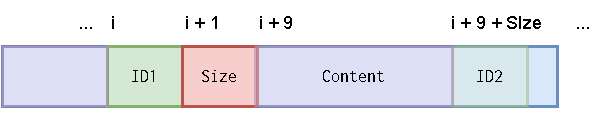
\includegraphics[width=0.5\linewidth]{figures/section.pdf}
    \caption{Memory byte representation of a \Wasm binary section, starting with a 1-byte section ID, followed by an 8-byte section size, and finally the section content.}
    \label{background:wasm:fig:section}
\end{figure}

\wrule{Custom Section (\texttt{00})}: Comprises two parts: the section name and arbitrary content. Primarily used for storing metadata, such as the compiler used to generate the binary (see lines 9 and 48 of \autoref{WASMExample}). This type of section has no order constraints with other sections and is optional. Compilers usually skip this section when consuming a \Wasm binary. 

\wrule{Type Section (\texttt{01})}: Contains the function signatures for functions declared or defined within the binary (see lines 3 to 6 in \autoref{WASMExample}). Functions may share the same function signature. This section must occur only once in a binary. It can be empty. 

\wrule{Import Section (\texttt{02})}: Lists elements imported from the host, including functions, memories, globals, and tables (see line 8 in \autoref{WASMExample}). This section is needed to enable code and data sharing with the host engine and other modules. It must occur only once in a binary. It can be empty.

\wrule{Function Section (\texttt{03})}: Details functions defined within the binary. It essentially maps Type section entries to Code section entries. The text format already maps the function index to its name, as shown in lines 12 to 38 of \autoref{WASMExample}. This section must occur only once in a binary and, it can be empty. 

\wrule{Table Section (\texttt{04})}: Groups functions with identical signatures to control indirect calls. It must occur only once in a binary. It can be empty. The example code in \autoref{WASMExample} does not include a Table Section.

\wrule{Memory Section (\texttt{05})}: Specifies the number and initial size of unmanaged linear memories (see line 40 in \autoref{WASMExample}). It must occur only once in a binary. It can be empty. 

\wrule{Global Section (\texttt{06})}: Defines global variables as managed memory for use and sharing between functions in the \Wasm binary (see line 42 of \autoref{WASMExample}). It must occur only once in a binary. It can be empty.

\wrule{Export Section (\texttt{07})}: Declares elements like functions, globals, memories, and tables for host engine access (see lines 44 and 45 of \autoref{WASMExample}). It must occur only once in a binary. It can be empty.

\wrule{Start Section (\texttt{08})}:  Designates a function to be called upon binary readiness, initializing the \Wasm program state before executing any exported functions. It must occur only once in a binary. It can be empty. The example code in \autoref{WASMExample} does not include a Start Section, i.e. there is no function to call when the binary is initialized.

\wrule{Element Section (\texttt{09})}: Contains elements to initialize the binary tables. It must occur only once in a binary. It can be empty. The example code in \autoref{WASMExample} does not include an Element Section.

\wrule{Code Section (\texttt{10})}: Contains the body of functions defined in the Function section. Each entry consists of local variables used and a list of instructions (see lines 12 to 38 in \autoref{WASMExample}). It must occur only once in a binary. It can be empty.

\wrule{Data Section (\texttt{11})}: Holds data for initializing unmanaged linear memory. Each entry specifies the offset and data to be placed in memory (see line 47 in \autoref{WASMExample}). It must occur only once in a binary. It can be empty.

\wrule{Data Count Section (\texttt{12})}: Primarily used for validating the Data Section. If the segment count in the Data Section mismatches the Data Count, the binary is considered malformed. The example code in \autoref{WASMExample} does not include a Data Count Section.
It must occur only once in a binary. It can be empty.


\vspace{2mm}
Due to its organization into a contiguous array of sections, a \wasm binary can be processed efficiently. 
For example, this structure allows compilers to speed up the compilation process through parallel parsing or just by ignoring \emph{Custom Sections}.
Additionally, the use of the LEB128\toolcite{https://en.wikipedia.org/wiki/LEB128} encoding of instructions of the \emph{Code Section} further compacts the binary. 
As a result, Wasm binaries are not only fast to validate and compile but also quick to transmit over a network.

\msubsection{\Wasm's runtime structure}
\label{background:wasm:execution}


The \Wasm runtime structure is described in the WebAssembly specification by enunciating 10 key components: the Store, Module Instances,  Table Instances, Export Instances, Import Instances, the Execution Stack, Memory Instances, Global Instances, Function Instances and Locals.  
These components are particularly significant in maintaining the state of a WebAssembly program during its execution. 
In the following, we provide a brief description of each runtime component.
Notice that, the runtime structure is an abstraction that serves to validate the execution of a \wasm binary.

\wrule{Store}: The WebAssembly store represents the global state and is a collection of instances of functions, tables, memories, and globals. Each of these instances is uniquely identified by an address, which is usually represented as an i32 integer.


\wrule{Module Instances}: A module instance is a runtime representation of a loaded and initialized WebAssembly module (the binary file described in \autoref{background:wasm:binary}). 
It contains the runtime representation of all the definitions within a module, including functions, tables, memories, and globals, as well as the module's exports and imports.


\wrule{Table instances}: A table instance is a vector of \emph{function instances} with the same signature. 
They are used to validate and support indirect function calls during runtime.
A table instance can be modified through table instructions from the function bodies.


\wrule{Export Instances}: Export instances represent the functions, tables, elements, globals or memories that are exported by a \wasm binary to the host environment. 

\wrule{Import Instances}: Import instances represent the functions, tables, elements, globals or memories that are imported into a module from the host environment. 

\wrule{The Execution Stack} holds typed values, labels and control frames, with labels handling block instructions, loops, and function calls.
Values inside the stack can be of the only static types allowed in Wasm 1.0, \texttt{i32} for 32 bits signed integer, \texttt{i64} for 64 bits signed integer, \texttt{f32} for 32 bits float and \texttt{f64} for 64 bits float.
Therefore, abstract types, such as classes, objects, and arrays, are not natively supported. 
Instead, during compilation, such types are transformed into primitive types and stored in the linear memory.

\wrule{Memory Instances} represent the unmanaged linear memory of a WebAssembly program, consisting of a contiguous array of bytes.
Memory instances are accessed with \texttt{i32} pointers (integer of 32 bits). 
Memory instances are usually bound in browser engines to 4Gb of size, and it is only shareable between the process that instantiates the \Wasm module and the binary itself.

\wrule{Global Instances}: A global instance is a global variable with a value and a mutability flag, indicating whether the global can be modified or is immutable.
Global variables are part of the managed data, i.e., their allocation and memory placement are managed by the host engine.
Global variables are only accessible by their declaration index, and it is not possible to dynamically address them. 


\wrule{Locals}: Locals are mutable variables that are local to a specific function instance, i.e. locals are only accessible through their index related to the executing function instance. As globals, locals are part of the managed data.

\wrule{Function Instances}: are closures over the runtime module instance.
A function instance groups locals and a function body.
Locals are typed variables that are local to a specific function invocation as previously discussed.
The function body is a sequence of instructions that are executed when the function is called.
Each instruction either reads from the stack, writes to the stack, or modifies the control flow of the function.
Recalling the example \wasm binary previously showed, 
% Functions
the local variable declarations and typed instructions that are evaluated using the stack can be appreciated between Line 7 and Line 32 in \autoref{WASMExample}. 
Each instruction reads its operands from the stack and pushes back the result. 
In the case of \autoref{WASMExample}, the result value of the main function is the calculation of the last instruction, \texttt{i32.add}. 
As the listing also shows, instructions are annotated with a numeric type.


\begin{definition}\label{managed_unmanaged}
    Along with this dissertation, as the work of Lehmann \etal \cite{usenixWasm2020}, we refer to managed and unmanaged data to differentiate between the data that is managed by the host engine and the data that is managed by the \Wasm program respectively. 
\end{definition}


\msubsection{\Wasm's control flow}

In \Wasm, a defined function instructions are organized into blocks, with the function's starting point serving as the root block. 
Unlike traditional assembly code, control flow structures in Wasm jump between block boundaries rather than arbitrary positions within the code. 
Each block might specify the required stack state before execution and the resulting stack state after its instructions have run. 
This stack state is used to validate the binary during compilation and to ensure that the stack is in a valid state before executing the block's instructions.
Blocks in Wasm are explicit, indicating, where they start and end.
By design, each block cannot reference or execute code from outer blocks.

Control flow within a function is managed through three types of break instructions: unconditional break, conditional break, and table break. 
Importantly, each break instruction is limited to jumping to one of its enclosing blocks.
%Loops in Wasm are specialized blocks that can be restarted using a break instruction. 
Unlike standard blocks, where breaks jump to the end of the block, breaks within a loop block jump to the block's beginning, effectively restarting the loop. 
To illustrate this, \autoref{background:wasm:block} provides an example comparing a standard block and a loop block in a Wasm function.


\begin{minipage}{0.95\linewidth}
   
   \begin{minipage}{0.45\linewidth}
      \lstset{
      language=WAT,
      style=WATStyle,
      breaklines=true, 
      %stepnumber=0,
      escapeinside={(*@}{@*)},
      numbers=none,
      postbreak=\mbox{\space},
      label=BlockExample}

   \begin{lstlisting}    
block
   block
      br 1 (*@\tikzmarkMap{2}{}{8.5}{2}{2cm}@*) ; Jump instructions are annotated with the depth of the block they jump to; 
   end (*@\tikzmarkMap{7}{}{8.5}{0}{2cm}@*)
end (*@\tikzmarkMap{1}{}{8}{3}{2cm}@*)
... (*@\tikzmarkMap{9}{}{8.5}{2}{2cm}@*)
   \end{lstlisting}
   \end{minipage}\hspace{1mm}
   \begin{minipage}{0.44\linewidth}
   \lstset{
      language=WAT,
      style=WATStyle,
      breaklines=true, 
      %stepnumber=0,
      escapeinside={(*@}{@*)},
      numbers=none,
      postbreak=\mbox{\space},
      label=LoopExample}

   \begin{lstlisting}    
loop (*@\tikzmarkMap{6}{}{8.5}{2}{2cm}@*)
   ...
   br 0 (*@\tikzmarkMap{5}{}{8.5}{2}{2cm}@*) ;first-order break;
   ... 
end (*@\tikzmarkMap{3}{}{8.5}{2}{2cm}@*) ; end instructions break the block and jump to next instruction; 
... (*@\tikzmarkMap{4}{}{8.5}{-2}{2cm}@*)
   \end{lstlisting}
   \end{minipage}
   \begin{tikzpicture}[remember picture,overlay]

      %\path (2.west) edge[<-, black] (1.west);
      %\path (3.west) edge[<-,  black] (4.west);
   
      \path (1.west) edge[<-, bend right, black] (2.west);
      %\path (1.west) edge[<-, bend right, gray] (7.west);
      %\path (9.west) edge[<-, bend right, gray] (1.west);
   
      \path (4.west) edge[<-, bend right, gray] (3.west);
      \path (6.west) edge[<-, bend left, black] (5.west);
      %\path (9.east) edge[<-, bend right, black] (4.east);
      %\path (7.east) edge[<-, bend right, black] (8.east);
   
      \end{tikzpicture}
      \centering
      \hrule
      \vspace{2mm}
      \captionof{lstlisting}{Example of breaking a block and a loop in \Wasm.}
      \label{background:wasm:block}
\end{minipage}
% Example


Each break instruction includes the depth of the enclosing block as an operand. 
This depth is used to identify the target block for the break instruction. 
For example, in the left-most part of the previously discussed listing, a break instruction with a depth of 1 would jump past two enclosing blocks.


\msubsection{\Wasm's ecosystem}
\label{background:wasm:ecosystems}

%\todo{Split in two sections. Do a new section on WebAssembly analysis.}
%\todo{Other WebAssembly tools section.}

\Wasm programs are tailored for execution in host environments, most notably web browsers. 
The \Wasm ecosystem is a diverse landscape, featuring a multitude of stakeholders and a comprehensive suite of tools to meet various requirements \cite{Avenger}. 
In this section, we delineate two key categories of tools within this ecosystem: compilers and executors. 
Compilers are responsible for converting source code into \Wasm binaries, while executors handle a range of tasks including validation, optimization, machine code transpilation, and actual execution of these \Wasm binaries. 
Executors are often found in browser clients, among other platform

\wrule{Compilers} transform source code into \Wasm binaries. 
For example, LLVM has offered \Wasm as a backend option since its 7.1.0 release\toolcite{https://github.com/llvm/llvm-project/releases/tag/llvmorg-7.1.0}, supporting a diverse set of frontend languages like C/C++, Rust, Go, and AssemblyScript\footnote{A subset of the TypeScript language}.
Significantly, a study by Hilbig et al. reveals that 70\% of \Wasm binaries are generated using LLVM-based compilers. 
In parallel developments, the KMM framework\toolcite{https://kotlinlang.org/docs/wasm-overview.html} has incorporated \Wasm as a compilation target, and the Javy approach\toolcite{https://github.com/bytecodealliance/javy} focuses on encapsulating JavaScript code within isolated \Wasm binaries. 
This latter is achieved by porting both the engine and the source code into a secure \Wasm environment. 
Similarly, Blazor also enables the compilation of C# code into \Wasm binaries for browser execution\footnote{\url{https://dotnet.microsoft.com/apps/aspnet/web-apps/blazor}}.

From a security standpoint, \Wasm programs are designed without a standard library and are prohibited from direct interactions with the operating system. Instead, the host environment offers a predefined set of functions that can be imported into the \Wasm program. 
It falls upon the compilers to specify which functions from the host environment will be imported by the \Wasm application.

\wrule{Browser} engines like V8\toolcite{https://chromium.googlesource.com/v8/v8.git} and SpiderMonkey\toolcite{https://spidermonkey.dev/} are at the forefront of executing \Wasm binaries in browser clients. 
These engines leverage Just-In-Time (JIT) compilers to convert \Wasm into machine code. 
This translation is typically a straightforward one-to-one mapping, given that \Wasm is already an optimized format closely aligned with machine code, as previously discussed in \autoref{background:wasm:binary}. 
For example, V8 just employs quick, rudimentary optimizations, such as constant folding and dead code removal, to guarantee fast readiness for a \wasm binary to execute \cite{10.1145/3282510}.

\wrule{Standalone engines:} \wasm has expanded beyond browser environments, largely due to the WASI\cite{WASI}. 
It standardizes the interactions between host environments and \Wasm modules through a POSIX-like interface.
\wasm compilers can generate binaries that use WASI.
Standalone engines can then execute these binaries in a variety of environments, including cloud, server, and IoT devices.
For example, standalone engines like WASM3\toolcite{https://github.com/wasm3/wasm3}, Wasmer\toolcite{https://wasmer.io/}, Wasmtime\toolcite{https://github.com/bytecodealliance/wasmtime}, WAVM\toolcite{https://github.com/WAVM/WAVM}, and Sledge\cite{Sledge} have emerged to support \Wasm and WASI. 
In a similar vein, Singh et al.\cite{WARDuino2019} introduced a virtual machine for \Wasm tailored for Arduino-based devices. 
Salim et al.\cite{trufflewasm} proposed TruffleWasm, an implementation of \Wasm hosted on Truffle and GraalVM. 
Additionally, SWAM\toolcite{https://github.com/satabin/swam} stands out as \Wasm interpreter implemented in Scala. 
Finally, WaVe\cite{wave} offers a \Wasm interpreter featuring mechanized verification of the \Wasm-WASI interaction with the underlying operating system.



\msubsection{WebAssembly's binary analysis}
\label{background:wasm:analysis}
As the WebAssembly ecosystem continues to grow, the need for robust tools to ensure its security and reliability has increased. 
To address this, a variety of tools have been developed that employ different strategies to identify vulnerabilities in \Wasm programs. 
In the following we provide a brief overview of the most relevant tools in this space w.r.t static and dynamic analysis, as well as specialized malware detection.

%% PATCH
\vspace{10mm}
\wrule{Static and dynamic analysis:} 
Tools like Wassail\cite{wassail}, SecWasm\cite{secwasm}, Wasmati\cite{wasmati}, and Wasp\cite{Wasp} leverage techniques such as information flow control, code property graphs, control flow analysis, and concolic execution to detect vulnerabilities in \wasm binaries. 
Remarkably, VeriWasm\cite{veriwasm} stands out as a static offline verifier specifically designed for native x86-64 binaries compiled from \Wasm. 
In the dynamic analysis counterpart, tools like TaintAssembly\cite{taintassembly}, Wasabi\cite{wasabi}, and Fuzzm\cite{fuzzm} offer similar functionalities in vulnerability detection. 
Stiévenart and colleagues have introduced a dynamic approach to slice \Wasm programs based on Observational-Based Slicing (ORBS)\cite{slicing, slicing2}. 
Hybrid methods have also gained traction, with tools like CT-Wasm\cite{ctwasm} enabling the verifiably secure implementation of cryptographic algorithms in \Wasm. 
% Finally, Wafl\cite{wafl} extends AFL++ to perform coverage-based fuzzing on \Wasm binaries.


\wrule{Specialized Malware Detection:} Cryptomalware have a wide presence in the web since the first days of \wasm.
The main reason is that mining algorithms using CPUs moved to \wasm for obvious performance reasons \cite{musch2019new}. 
In cryptomalware detection, tools like MineSweeper\cite{Minesweeper}, MinerRay\cite{MinerRay}, and MINOS\cite{MINOS} utilize static analysis through machine learning techniques to detect browser cryptomalwares. 
Conversely, tools like SEISMIC\cite{SEISMIC}, RAPID\cite{RAPID}, and OUTGuard\cite{outguard} seek the same goal with dynamic analysis techniques.
Remarkably, VirusTotal\toolcite{https://www.virustotal.com}, packaging more than 60 commercial antivirus as back-boxes, detects cryptomalware in \wasm binaries.


\msubsection{\Wasm's security}


While \Wasm is engineered to be deterministic, well-typed, and to adhere to a structured control flow, the ecosystem is still emerging and faces various security vulnerabilities. 
These vulnerabilities pose risks to both the consumers and the \Wasm binaries themselves. 
Side-channel attacks, in particular, are a significant concern. 
For example, Genkin et al. have shown that \Wasm can be exploited to exfiltrate data through cache timing-side channels \cite{Genkin2018DrivebyKC}. 
Similarly, research by Maisuradze and Rossow demonstrates the feasibility of speculative execution attacks on \Wasm binaries \cite{ret2spec}. 
Rokicki \etal further reveal the potential for port contention side-channel attacks on \Wasm binaries in browsers \cite{10.1145/3488932.3517411}.
Additionally, studies by Lehmann et al. and Stiévenart and colleagues indicate that vulnerabilities in C/C++ source code can propagate into \Wasm binaries \cite{usenixWasm2020, DeRoover2022}. 
This dissertation introduces a comprehensive set of tools aimed at preemptively enhancing \Wasm security through Software Diversification and at improving testing rigor within the ecosystem.





\msection{Software diversification}
\label{sota:sw}

%%ORIGINAL
Software diversification involves the synthesis, reuse, distribution, and execution of different, functionally equivalent programs so-called software variants. 
As outlined in Baudry \etal's survey \cite{natural_diversity}, Software Diversification falls into five usage categories: reusability \cite{pohl2005software},performance \cite{10.1145/2025113.2025133}, fault tolerance \cite{1659219}, software testing \cite{Chen2010AdaptiveRT}, and security \cite{cohen1993operating}. 
Our work specifically contributes to the last two categories.
Based on the works of Cohen \etal \cite{cohen1993operating}, Forrest \etal \cite{595185}, Jackson \etal \cite{jackson} and Baudry \etal \cite{natural_diversity}, this section presents core concepts and related works. 



Software variants refer to functionally equivalent versions of an original program, produced through Software Diversification at various stages of the software lifecycle, from dependencies (coarse-grained) to machine code levels (fine-grained).
The main goal of Software Diversification is to increase the cost of exploitation by making software less predictable. 
Diversification may be natural \cite{natural_diversity} or automatic \cite{offensive_div}. 
Natural diversity refers to the side effect of humans creating software variants using different programming languages, compilers, and operating systems \cite{natural_diversity}, all of which adhere to the initial requirements. 
The software market and competition typically address the creation of natural diversity. 
For example, Firefox and Chrome web browsers demonstrate natural diversity due to their practical differences in implementation and performance, despite serving the same purpose. 
This logic extends to operating systems, database engines, virtual machines, and application servers \cite{natural_diversity}. 
Natural diversity significantly aids in system security, as different variants are not susceptible to the same vulnerabilities \cite{781031, 10.5555/1009382.1009753}. 
Unlike N-Version programming \cite{6312924}, natural diversity organically emerges over decades. 
In other words, while it does not require the allocation of additional human efforts, natural diversity cannot be automatically generated. 
This is because it is a side effect of the software development process.
Given that \Wasm is a relatively new technology, natural diversity is presently not a feasible option. 
Hence, for \Wasm, feasible options are systematic and automatic diversification approaches.



\msubsection{Automatic generation of software variants}
\label{artificial_diversity}

The concept of automatic software variants starts with Randell's 1975 work \cite{10.1145/390016.808467}, which put forth the notion of artificial fault-tolerant instruction blocks. 
Artificial Software Diversification, as proposed by Cohen and Forrest in the 1990s \cite{cohen1993operating, 595185}, gets its development through rewriting strategies. 
These strategies consist of rule sets for modifying software components to create functionally equivalent, yet distinct, programs. 
Rewriting strategies typically take the form of tuples: \texttt{instr1 => (instr2, instr3, ...)}, where \texttt{instr} represents the original code and \texttt{(instr2, instr3, ...)} denotes the functionally equivalent code.


\begin{strategy}[Rewriting strategy]
    \label{rewriting_strategy}
    The automatic creation of Software Diversification begins with creating rewriting rules.
    A rewriting rule refers to a functionally equivalent substitution for a code segment, manually written. 
    These rules can be applied at varying levels, from coarse to fine-grained. 
    This can range from the program dependencies level \cite{Harrand1650630} to the instruction level \cite{offensive_div}. 
    For example, Cleemput et al.~\cite{Cleemput2012} and Homescu et al.~\cite{homescu2013profile} inject NOP instructions to yield statically varied versions at the instruction level. 
    Here, the rewriting rule is represented as \texttt{instr => (nop instr)}, signifying a \texttt{nop} operation preceding the instruction.


    %Although the studies by Cleemput et al. and Homescu et al. are easily applicable to \Wasm, this specific strategy may fall under the \emph{non preserved} category since \Wasm typically compiles later. 
    %This implies that JIT compilers could nullify this diversification strategy by merely applying straightforward optimizations.
\end{strategy}



\begin{strategy}[Instruction Reordering]
    \label{instruction_reordering}
    This strategy reorders instructions in a program.
    For example, variable declarations may change if compilers reorder them in the symbol tables. 
    This prevents static examination and analysis of parameters and alters memory locations. 
    In this area, Bhatkar \etal \cite{bhatkar03, bhatkar2005efficient} proposed the random permutation of variable and routine order for ELF binaries.
    Such strategies are not implemented for \Wasm to the best of our knowledge.
\end{strategy}


\begin{strategy}[Adding, Changing, Removing Jumps and Calls]
    \label{jumps}
    This strategy generates program variants by adding, changing, or removing jumps and calls in the original program. 
    Cohen \cite{cohen1993operating} primarily illustrated this concept by inserting random jumps in programs. Pettis and Hansen \cite{pettisochhansen} suggested splitting basic blocks and functions for the PA-RISC architecture, inserting jumps between splits.
    Similarly, Crane \etal~\cite{crane2015thwarting} de-inlined basic blocks of code as an LLVM pass. 
    In their approach, each de-inlined code transforms into semantically equivalent functions that are randomly selected at runtime to replace the original code calculation. 
    On the same topic, Bhatkar \etal \cite{bhatkar2005efficient} extended their previous approach \cite{bhatkar03}, replacing function calls with indirect pointer calls in C source code, allowing post-binary reordering of function calls. 
    In the \Wasm context, the most analogous work is Wobfuscator \cite{wobfuscator}.
    Wobfuscator, a JavaScript obfuscator, substitutes pieces of JavaScript code with \Wasm code, e.g., numeric calculi.
    This strategy effectively uses the interleaving of calls between JavaScript and \Wasm to provide JavaScript variants.
\end{strategy}


\begin{strategy}[Program Memory and Stack Randomization]
    \label{mem_strategy}
    This strategy alters the layout of programs in the host memory. 
    Additionally, it can randomize how a program variant operates its memory. 
    The work of Bhatkar \etal \cite{bhatkar03, bhatkar2005efficient} proposes to randomize the base addresses of applications and library memory regions in ELF binaries. 
    Tadesse Aga and Autin \cite{aga2019smokestack}, and Lee \etal \cite{lee2021savior} propose a technique to randomize the local stack organization for function calls using a custom LLVM compiler.
    Younan \etal \cite{Younan2006} suggest separating a conventional stack into multiple stacks where each stack contains a particular class of data. 
    On the same topic, Xu \etal \cite{xu2020merr} transforms programs to reduce memory exposure time, improving the time needed for frequent memory address randomization. 
    This makes it very challenging for an attacker to ignore the key to inject executable code. 
    This strategy disrupts the predictability of program execution and mitigates certain exploits such as speculative execution.
    No work has been found that explicitly applies this strategy to \Wasm.
    %Yet, transforming \Wasm binaries inherently randomizes the memory layout.
    %Consequently, memory accesses are randomized as these binaries are further JITed to machine code in the majority of cases.
\end{strategy}

\begin{strategy}[ISA Randomization and Simulation]
    \label{isa_rand}

    This strategy involves using a key to cipher the original program binary into another encoded binary. 
    Once encoded, the program can only be decoded at the target client, or it can be interpreted in the encoded form using a custom virtual machine implementation. 
    This technique is strong against attacks involving code inspection. 
    Kc \etal \cite{Kc03}, and Barrantes \etal \cite{barrantes2003randomized} proposed seminal works on instruction-set randomization 
    to create a unique mapping between artificial CPU instructions and real ones.
    On the same topic, Chew and Song \cite{Chew02mitigatingbuffer} target operating system randomization. They randomize the interface between the operating system and the user applications.
    Courouss{\'e} \etal~\cite{courousse2016runtime} implement an assembly-like DSL to generate equivalent code at runtime in order to increase protection against side-channel attacks. 
    Their technique generates a different program during execution using an interpreter for their DSL.
    Generally, \emph{ISA randomization and simulation} usually faces a performance penalty, especially for \Wasm, due to the decoding process as shown in WASMixer evaluation \cite{wasmixer}.
\end{strategy}


\begin{strategy}[Code obfuscation]
    \label{obfusscation}
    Code obfuscation can be seen as a simplification of \emph{ISA randomization}. 
    The main difference between encoding and obfuscating code is that the former requires the final target to know the encoding key while the latter executes as is in any client \cite{10.1145/3176258}. 
    Yet, both strategies aim to tackle static reverse engineering of programs.
    In the context of \Wasm, Romano \etal \cite{wobfuscator} proposed an obfuscation technique, wobfuscator, for JavaScript in which part of the code is replaced by calls to complementary \Wasm functions.
    Yet, wobfuscator targets JavaScript code, not \Wasm binaries.
    %BREWasm \cite{BREWasm}, as a generic rewriting tool, showcases how to obfuscate \Wasm binaries. 
\end{strategy}



\begin{strategy}[Enumerative synthesis]
    \label{enumerative_synthesis}
    Enumerative synthesis is a fully automated and systematic approach to generate program variants.
    It examines all possible programs specific to a given language.
    The process of enumerative synthesis commences with a piece of input program, typically a basic block.
    Incrementally, using a defined grammar, it generates all programs of size $n$.
    A generated program is then checked for equivalence to the original program, either by using a test suite or a theorem solver.
    If the generated variant is proven, it is added to the variant's collection.
    The procedure continues until all potential programs have been explored.
    This approach proves especially effective when the solution space is relatively small or can be navigated efficiently.
    Jacob and colleagues \cite{jacob2008superdiversifier} implemented this strategy for x86 programs.
    They named this technique superdiversification, drawing parallels to superoptimization \cite{Massalin1987}.
    Since this strategy fully explores a program's solution space, it contains the aforementioned strategies as special cases.
    The application of enumerative synthesis to \Wasm has not been explored. 
\end{strategy}


\msubsection{Equivalence Checking}
\label{equivalence:checking}


Equivalence checking between program variants is a vital component for any program transformation task, ranging from checking compiler optimizations \cite{LeCompilers} to the artificial synthesis of programs discussed in this chapter. 
It proves that two pieces of code or programs are functionally equivalent \cite{churchill2019}. 
We can roughly simplify the checking process with the following property: 
two programs are deemed equivalent if they generate identical outputs when given identical inputs from a closed collection of inputs \cite{10.1145/2814270.2814319}.
We adopt this definition of \emph{functional equivalence modulo input} throughout this dissertation. 
In Software Diversification, equivalence checking seeks to preserve the original functionality of programs while varying observable behaviors. 
Two programs, for instance, can differ statically and still compute the same result. 
We outline three methods to check variant equivalence: by construction, check modulo tests and prove-driven equivalence checking.


\begin{checking}[Equivalence by construction]
    \label{check_by_construction}
    The equivalence property can be guaranteed by construction.
    As previously mentioned, Cleemput \etal \cite{Cleemput2012} and Homescu \etal \cite{homescu2013profile} exemplify transformation strategies that generate semantically equivalent program variants. 
    These variants are equivalent by construction. 
    In their case, NOP instructions produce statically different variants. 
    NOP operations, interleaved by any other type of original instruction, serve as a functionally equivalent replacement. 
    However, developer errors may occur during this process, necessitating further validation.
    The test suite of the original program can serve as a check for the variant. 
\end{checking}

\begin{checking}[Checking modulo tests]
    \label{check_by_tests}

    The process of checking modulo tests involves utilizing a test suite to confirm the equivalence of program variants \cite{10.1007/s10710-013-9195-8, 10.1145/2610384.2610415}. 
    When a program variant successfully passes the test suite, it is determined equivalent to the original. 
    It is reasonable to assume that projects prioritizing quality and security are likely to have a robust test suite that facilitates this type of equivalence verification.
    However, this technique's effectiveness is bounded by the necessity for a preexisting test suite. 
    Yet, as an alternative, fuzzers can be used to automatically generate tests \cite{zalewski2017american}.
    Fuzzers operate by randomly generating inputs that lead to different observable behaviors. 
    If a variant produces a different output from two identical inputs, it is not equivalent to the original program. 
    Fuzzers' primary drawback is their time-consuming nature and the requirement for manually introducing oracles.
    Recent advancements in the field of machine learning have led researchers to explore the application of neural networks in verifying program equivalence.
    Zhang and his team's work provides an example of this, where Large Language Models are used to generate reference oracles and test cases \cite{2023arXiv230514591Z}.
    Despite its effectiveness, this method attains an accuracy rate of just 88\%, which falls short of providing complete verification.

\end{checking}

\begin{checking}[Formal checking]
    \label{check_by_smt}
    In the absence of a test suite or a technique that inherently implements the equivalence property, the works mentioned earlier use theorem solvers (SMT solvers) \cite{SMT_solver} to prove the equivalence of program variants. 
    The central idea for SMT solvers is to convert the two code variants into mathematical formulas. 
    The SMT solver then checks for counter-examples \cite{kesseli2018counterexample}. 
    When it finds a counter-example, there is an input for which the two mathematical formulas yield different outputs. 
    The primary limitation of this technique is that not all algorithms can be translated into a mathematical formula, such as loops. 
    Nevertheless, this technique is frequently used for checking no-jump-programs like basic block and peephole replacements \cite{SuperoptimizationScaling}.
\end{checking}



\msubsection{Variants deployment}
\label{deployment}
Program variants, once generated and verified, may be used in two primary scenarios: Randomization or Multivariant Execution (MVE) \cite{jackson}. 


\begin{strategy}[Randomization]
    \label{randomization}
    In the context of our work, the term \emph{Randomization} denotes a program's ability to present different variants to different clients. 
    In this setup, a program, chosen from a collection of variants (referred to as the program's variant pool), is assigned to a random client during each deployment. 
    Jackson \etal \cite{jackson} define the variant pool in Randomization as herd immunity, as vulnerable binaries can only affect a segment of the client community. 
    El-Khalil and colleagues \cite{ElKhalil2004} suggest employing a custom compiler to generate varying binaries from the compilation process. 
    They adapt a version of GCC 4.1 to partition a conventional stack into several component parts, termed multistacks. 
    Similarly, Singhal and colleagues, propose Cornucopia \cite{cornucopia}.
    Cornucopia generates multiple variants of a program by using different compiler flag combinations.
    Aga and colleagues propose the generation of program variants through the randomization of its data layout in memory\cite{aga2019smokestack}. 
    This method allows each variant to operate on the same data in memory but at different memory offsets. 
    Randomization can also be applied to virtual machines and operating systems. On this note, Kc \etal \cite{Kc03} establish a unique mapping between artificial CPU instructions and actual ones, enabling the assignment of various variants to specific target clients. 
    In a similar vein, Xu \etal \cite{xu2020merr} recompile the Linux Kernel to minimize the exposure time of persistent memory objects, thereby increasing the frequency of address randomization.
\end{strategy}


\begin{strategy}[Multivariant Execution (MVE)]
    Multiple program variants are composed into a single binary, known as a multivariant binary \cite{cox06}. 
    Each multivariant binary is randomly deployed to a client.
    Then, the multivariant binary executes its embedded program variants at runtime. 
    These embedded variants can either execute in parallel to check for inconsistencies, or as a single program to randomize execution paths \cite{bhatkar03}. 
    Bruschi and colleagues extend the concept of executing two variants in parallel, introducing non-overlapping and randomized memory layouts \cite{bruschi2007diversified}. 
    At the same time, Salamat \etal modify a standard library to generate 32-bit Intel variants. 
    These variants have a stack that grows in the opposite direction, allowing for the detection of memory inconsistencies \cite{salamat2007stopping}. 
    Davi and colleagues propose Isomeron, an approach for execution-path randomization \cite{davi2015isomeron}. 
    Isomeron operates by simultaneously loading the original program and a variant. 
    It then uses a coin flip to determine which copy of the program to execute next at the function call level. 
    Previous works have highlighted the benefits of limiting execution to only two variants in a multivariant environment. 
    Agosta and colleagues, as well as Crane and colleagues, used more than two generated programs in the multivariant composition, thereby randomizing software control flow at runtime \cite{agosta2015meet, crane2015thwarting}. 
    Both strategies have proven effective in enhancing security by addressing known vulnerabilities, such as Just-In-Time Return-Oriented Programming (JIT-ROP) attacks \cite{jackson2011compiler} and power side-channel attacks \cite{amarilli2011can}. 
    Lastly, only Voulimeneas \etal \cite{voulimeneas2021dmvx} have recently proposed a multivariant execution system that enhances security by parallelizing the execution of variants across different machines.
\end{strategy}


\msubsection{Measuring Software Diversification}
\label{measuring_diversification}
Measuring Software Diversification presents a significant challenge. 
The size of the variant space does not necessarily correlate with a variant's capacity to fulfill an objective such as hardening attacks by making systems less predictable \cite{cohen1993operating}. 
Ideally, real scenarios would provide the most accurate measurement of diversification, e.g., demonstrating a variant's effectiveness under specific attacks. 
However, such an approach is not always feasible, i.e., Software Diversification is a preventive strategy. 
Hence, a combination of static and dynamic metrics is required for measuring Software Diversification.

\begin{strategy}[Static comparison of variants]
    \label{static_based}
    Static metrics are used to measure the diversity of programs without needing execution. 
    The fundamental concept entails comparing variant source codes or binary codes to determine how diverse they are. 
    Usually, comparing variants means defining a distance metric between programs \cite{10.1145/2814270.2814319} where the more different the programs are, the greater the distance. 
    At the low-level of bytecode instructions, for example, these metrics include counting instructions \cite{10.1007/978-3-642-00730-9_10}, Levenshtein distance \cite{DBLP:journals/corr/abs-2111-09934}, and global alignments \cite{CROW}. 
    On the other hand, at the high-level of source code, these metrics often rely on Abstract Syntax Tree (AST) diffing, such as GUMtree-based distances \cite{gumtree} or machine learning inference \cite{203634}. 
    As an example of measuring the diversification, Bostani \etal \cite{Bostani2021EvadeDroidAP} illustrate the use of static distances in guiding the generation process of variants. 
    They categorize the space of Android applications into malware and goodware. 
    Then, they create malware variants by employing a static distance metric to approach the goodware group as closely as possible, thus successfully evading malware classifiers.
\end{strategy}

\begin{strategy}[Dynamic comparison of variants]
    \label{trace_based}
    Static comparisons between variants inherently have limitations. 
    For example, two variants may show differences at the source code level but exhibit identical behavior during execution. 
    Take the addition of \texttt{nop} operations to a program as an instance. 
    Despite source code level differences, the variant and the original program execute identical instructions, leading to similar behaviors modulo input. 
    Measuring Software Diversification primarily aims to demonstrate variant-specific observabilities. 
    While static differences are observable, runtime information holds complementary relevance \cite{yao2018anomaly}. 
    Therefore, dynamic metrics are essential to assess the diversity of variants. 
    For instance, Forrest \etal \cite{forrest_system_call} were pioneers in classifying program behaviors by analyzing their system call traces using n-grams profiling. 
    Cabrera \etal used a global alignments approach to gauge the diversity of JavaScript bytecode traces within the Chrome browser \cite{STRAC}. 
    Fang \etal proposed a method to counteract JavaScript obfuscation techniques used in malicious code, by analyzing dynamic information captured from V8 bytecode traces \cite{8482113}. 
    Dynamic metrics are primarily employed to cluster similar behaviors.
    Following the same logic, the diversity is greater when the difference between behaviors is larger. 
    Notice that, dynamic metrics can be difficult due to the expense of program execution or the complication of required user interaction. 
    On the other hand, malware programs, which usually do not require user interaction, are simpler to evaluate in controlled environments before actual deployment.

\end{strategy}

In the context of \Wasm, there exist no explicit works on Software Diversification.
Consequently, previous metrics have not been directly applied to measure diversification in \Wasm binaries.
However, in other domains, such as the analysis of \Wasm binaries, several studies have employed static metrics.
For example, VeriWasm quantifies attack-based patterns, stating that a \Wasm binary is more secure with a lower pattern count \cite{veriwasm}.
This metric might potentially serve as a guide during variant generation.
In the field of malware detection, MINOS \cite{MINOS} proposes transforming \Wasm binaries into grayscale images.
They then employ convolutional neural networks to identify malware, where an increased similarity to a malware image increases the probability of the binary being malware.
Regarding the dynamic comparisons, Wang \etal's study \cite{SEISMIC} profiles \Wasm instructions during runtime to identify malicious behavior.


\msubsection{Offensive or Defensive assessment of diversification}
\label{offensive_definition}

Lundquist and colleagues \cite{offensive_div} distinguish Software Diversification into two categories: Defensive and Offensive Diversification. 
On the one hand, Defensive Software Diversification introduces unpredictability in system behavior. 
By making software less predictable, defensive Software Diversification aims to proactively deter attacks, acting as a complementary strategy to other, more reactive, security measures. 
The majority of previously discussed works in this section contribute to defensive diversification.
Yet, Software Diversification that aims to create diverse harmful programs is considered Offensive Diversification \cite{fred1986computer}.


\begin{strategy}[Offensive Diversification]   
    Offensive Diversification is conceptually equal to Defensive Software Diversification.
    Yet, in an offensive context, one may apply diversification techniques to malware or other malicious codes to evade detection by security software \cite{8714698}.
    One might equate Offensive Diversification with Code obfuscation, if its purpose shifts from preventing reverse engineering by malicious actors, to evading detection by malware analysis systems.
    
    
\end{strategy}


Malicious actors may employ previously discussed diversification strategies to evade detection \cite{castro2019aimed}.
For instance, in the Web context, Weihang \etal propose to randomly transform HTML elements of web pages to evade advertisement blockers \cite{webranz}.
Over time, evasion techniques have evolved in both complexity and sophistication \cite{Aghakhani2020WhenMI}.
Chua \etal \cite{chua}, for instance, suggested a framework for automatically obfuscating the source code of Android applications using method overloading, opaque predicates, try-catch, and switch statement obfuscation, resulting in multiple versions of identical malware.
Moreover, machine learning approaches have been used to develop evasive malware \cite{2021arXiv211111487D}, drawing on a corpus of pre-existing malware \cite{Bostani2021EvadeDroidAP}.
These methods aim to thwart static malware detectors, yet, more advanced techniques focus on evading dynamic detection mostly by employing throttling \cite{Lu2013WeaknessesID, payer2014embracing}.


The term Offensive Software Diversification may seem counterintuitive.
Yet, such approaches measure the resilience and accuracy of security systems. 
This is an almost unexplored area in \Wasm, posing a threat to malware detection accuracy. 
Specifically, only Bhansali \etal seminal work\cite{10.1145/3507657.3528560} has demonstrated that a cryptomining algorithm's source code can evade pre-existing malware detection methods. 
More recently, Madvex \cite{madvex} has sought to obfuscate \Wasm binaries to achieve malware evasion, but this approach is limited to altering only the code section of \Wasm binaries.



\msection{Open challenges for Software Diversification}
\label{sota:openchallenges}
As outlined in \autoref{background:wasm:challenges}, our primary motivation for the contributions of this thesis is the open issues within the \Wasm ecosystem. 
We see potential in employing Software Diversification to address them. 
Based on our previous discussion, we highlight several open challenges in the realm of Software Diversification for \Wasm. 
First, \Wasm, being an emerging technology, is in the process of implementing defensive measures. 
In addition, while measures for \Wasm can be standardized, the implementation of these standards across the ecosystem is naturally slow. 
Therefore, applying Software Diversification directly to the generation of \Wasm binaries, according to any given specification, could serve as a valuable strategy to lessen the impact of vulnerabilities.
Second, despite the abundance of related work on software diversity, its exploration in the context of \Wasm remains limited. 
This thesis is the first to investigate Software Diversity in depth for the emerging \Wasm ecosystem.
Third, both randomization and multivariant execution remain largely unexplored within the \Wasm context. 
The deployment of Software Diversification in \Wasm poses unique challenges. 
\Wasm ecosystems are remarkably dynamic. 
Web browsers and FaaS platforms serve as prime examples. 
In these environments, \Wasm binaries are served millions of times simultaneously to the former, while new \Wasm binaries are cold-spawned and executed upon each user request in the latter. 
Thus, designing practical Software Diversification for \Wasm requires careful consideration of the deployment environment. 
Last but not least, research on malware detection, as discussed in \autoref{background:wasm:analysis}, suggests that offensive diversification may assist in evaluating the resilience and accuracy of \Wasm's security systems.



\msection{Exploiting Software Diversification}

\msubsection{Defensive Diversification}

\msubsection{Offensive Diversification}

%\section{Contributions of this thesis to Software Diversification for \Wasm}


\chapter{Automatic Software Diversification for WebAssembly}
\label{tech}
\todo{Start here. 4 pages each and 2 pages discussion. Target 20 pages.}



The work of Hilbig et al. \cite{Hilbig2021AnES} in 2021 influences our design decisions. According to their work, 70\% of the \wasm\ binaries in the wild are created with LLVM-based compilers. Therefore, we provide artificial software diversity for \wasm\ through LLVM. 
Other solutions would have been to diversify at the source-code level or the \wasm\ binary level. However, these facts would limit the applicability of our work.
Our approach is more general as diversification also will work for other LLVM backends.

LLVM is a compound of three main components \cite{llvmofficialweb}. First, the frontend (compilers such as clang and rustc) converts the program source code to LLVM intermediate representation (LLVM IR). Second, optimization and transformation processes improve the LLVM IR. Third and final, the backend component is in charge of generating the target machine code. In \autoref{diagrams:generic} we show how we use the LLVM pipeline in our contributions, which are highlighted as dashed squares.

\begin{figure*}[h]
    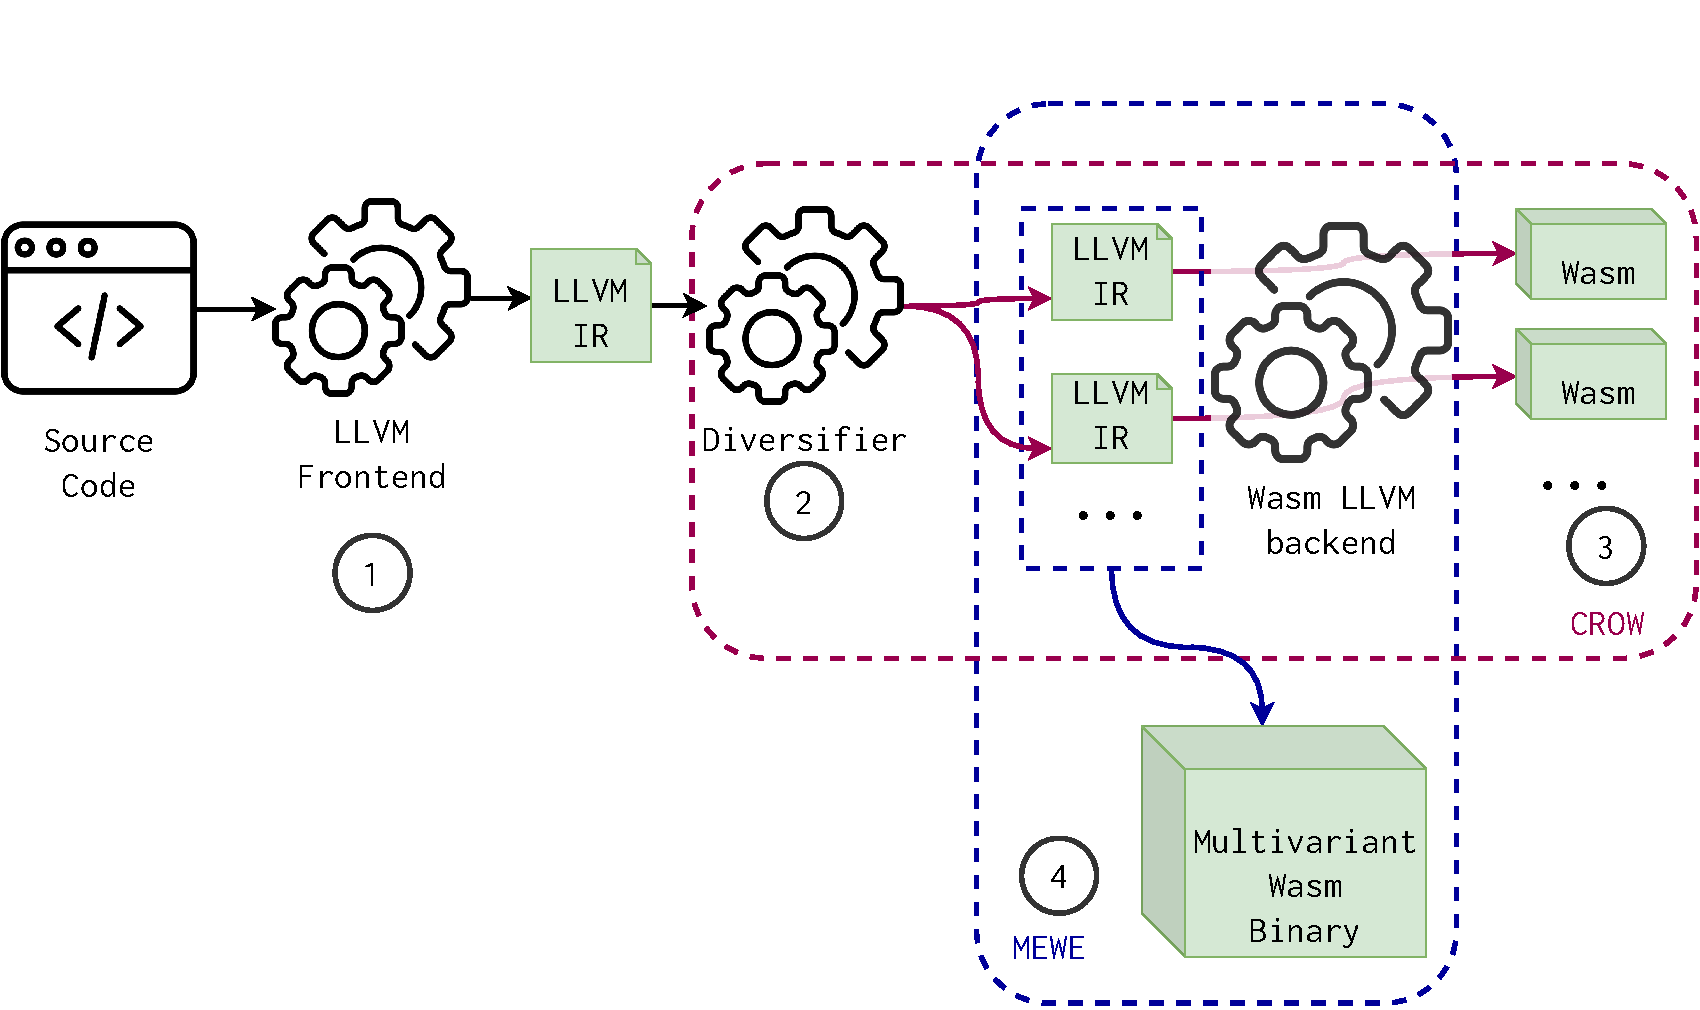
\includegraphics[width=\linewidth]{diagrams/architecture.pdf}
    \caption{Generic workflow to create \wasm\ program variants.}
    \label{diagrams:generic}
\end{figure*}



The global workflow in \autoref{diagrams:generic} starts by receiving the source code. Then the LLVM frontend transforms it into LLVM IR representation \step{1}. 
We alter the LLVM pipeline that compiles source code to Wasm by introducing a diversifier component.  

The diversifier generates LLVM IR variants from the output of the frontend \step{2}. 
The LLVM IR variants are inputs for our customized Wasm backend. 
The diversifier and the custom Wasm LLVM backend compose CROW, which creates \wasm\ program variants out of a source code program \step{3}. 
In addition, an orthogonal tool comes from the generation of LLVM IR variants at Step~\step{2}. MEWE  \cite{MEWE}, merges and creates multivariant binaries to provide MVE for \wasm\ \step{4}.  

\begin{figure}[h]
	\centering
	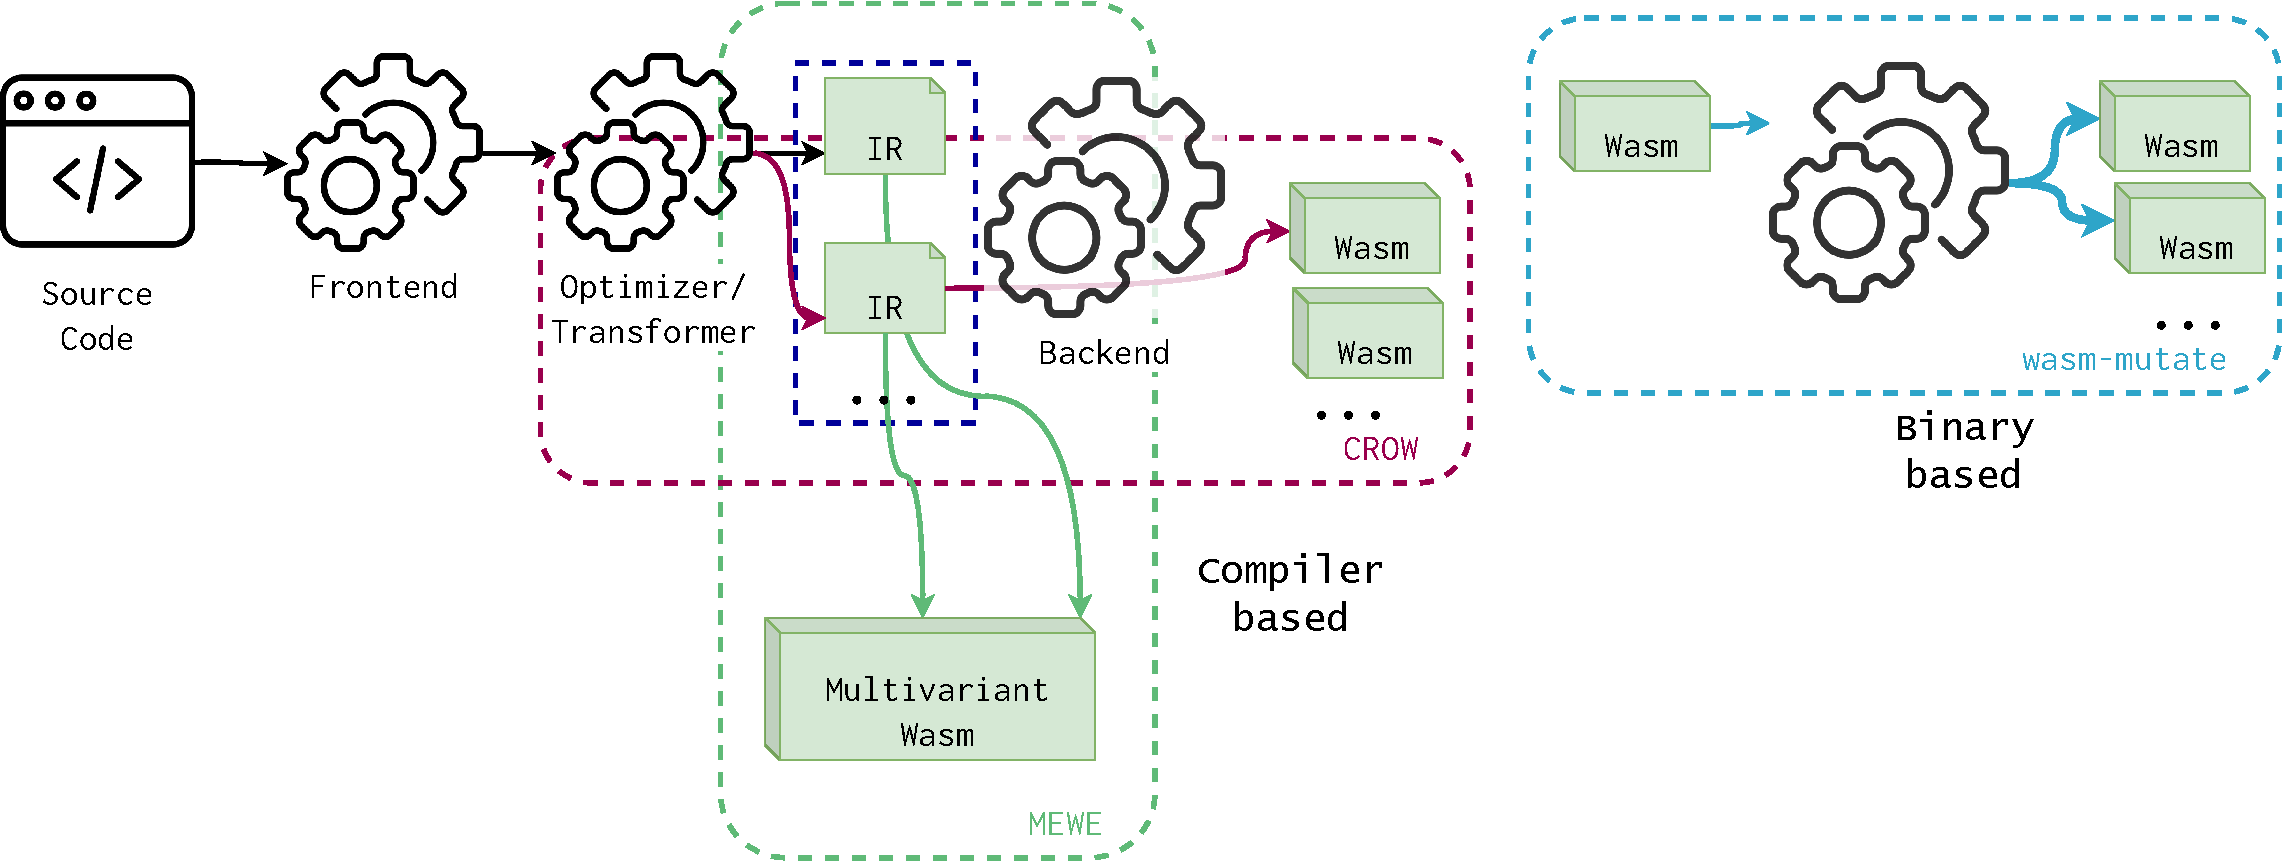
\includegraphics[width=1.0\textwidth]{figures/landscape.pdf}
	\caption{Approach landscape.}
	\label{fig:approach_landscape}
\end{figure}

\section{Compiler based approaches}
\msubsection{CROW: Code Randomization of WebAssembly}
\label{section:crow}

% Overview
This section describes the red squared tooling in \autoref{diagrams:generic} named CROW  \cite{CROW}. CROW is a tool tailored to create semantically equivalent \wasm\ variants from an LLVM front-end output.
Using a custom Wasm LLVM backend, it generates the Wasm binary variants.


In \autoref{diagrams:crow}, we describe the workflow of CROW to create program variants.
The Diversifier in CROW is composed by two main processes, \textit{exploration} and \textit{combining}. 
The \emph{exploration} process operates at the instruction level for each function in its input LLVM.
For all LLVM instructions, CROW produces a collection of functionally equivalent code replacements.   
In the \emph{combining} stage, CROW assembles the code replacements to generate different LLVM IR variants.
CROW generates the LLVM IR variants by traversing the power set of all possible combinations of code replacements.
Finally, the custom Wasm LLVM backend compiles the assembled LLVM IR variants into \wasm\ binaries.
In the following text, we describe our design decisions. All our implementation choices are based on one premise: \emph{each design decision should increase the number of \wasm\ variants that CROW creates.}
%\subsection*{Overview}

\begin{figure*}[h]
    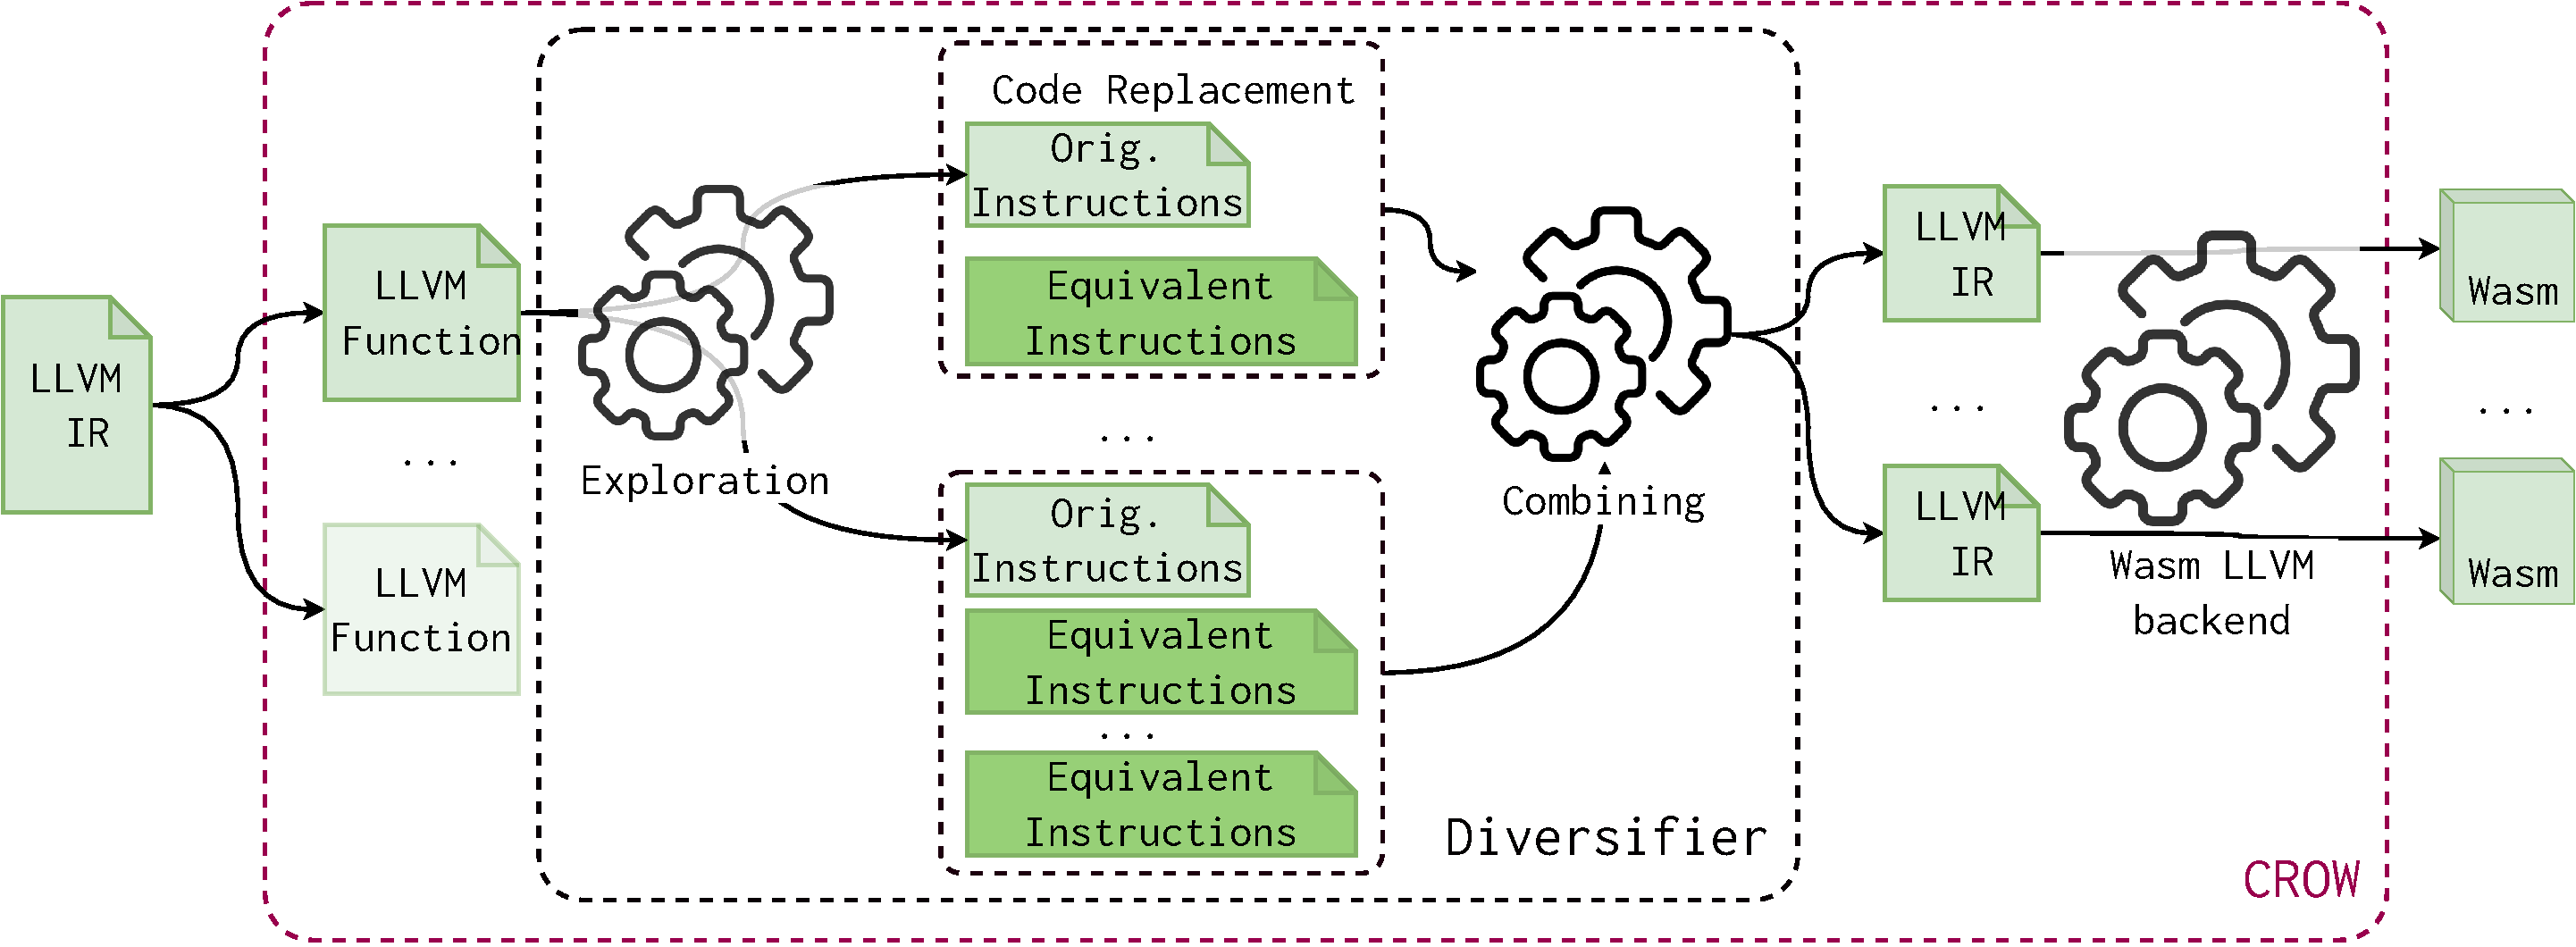
\includegraphics[width=\linewidth]{diagrams/generation/crow.drawio.pdf}
    \caption{CROW components following the diagram in \autoref{diagrams:generic}. CROW takes LLVM IR to generate functionally equivalent code replacements. Then, CROW assembles program variants by combining them.}
    \label{diagrams:crow}
\end{figure*}


%CROW operates at the code block level, taking them from the functions defined inside the input LLVM bitcode module. 
%In addition, the retargeted superoptimizer is in charge of finding the potential places in the original code blocks where a replacement can be applied. Finally, we use the enumerative synthesis strategy of the retargeted superoptimizer to generate code replacements.
%The code replacements generated through synthesis are verified, according to \autoref{def:functional-equivalence}, by internally using a theorem prover. 

\msubsection{Exploration}
%\subsection*{Variants' generation}

The primary component of CROW's exploration process is its code replacements generation strategy. The diversifier implemented in CROW is based on the proposed superdiversifier of Jacob \etal \cite{jacob2008superdiversifier}.
A superoptimizer focuses on \emph{searching} for a new program that is faster or smaller than the original code while preserving its functionality.
The concept of superoptimizing a program dates back to 1987, with the seminal work of Massalin \cite{Massalin1987} which proposes an exhaustive exploration of the solution space. The search space is defined by choosing a subset of the machine's instruction set and generating combinations of optimized programs, sorted by code size in ascending order. If any of these programs is found to perform the same function as the source program, the search halts. On the contrary, a superdiversifier keeps all intermediate search results despite their performance. 

% Why and main change
We use the superdiversifier idea of Jacob and colleagues to implement CROW because of two main reasons.
First, the code replacements generated by this technique outperform diversification strategies based on handwritten rules. Concretely, we can control the quality of the generated codes. Besides, CROW always generates equivalent programs because it is based on a solver to check for equivalence. 
Second, there is a battle-tested superoptimizer for LLVM, Souper \cite{Sasnauskas2017Souper:Superoptimizer}. This latter makes it feasible the construction of a generic LLVM superdiversifier. 

% This paragraph is hard to read
% How Souper works and why we can modify if
% Souper works as follows.
We modify Souper to keep all possible solutions in their searching algorithm.
Souper builds a Data Flow Graph for each LLVM integer-returning instruction. 
Then, for each Data Flow Graph, Souper exhaustively builds all possible expressions from a subset of the LLVM IR language.
Each syntactically correct expression in the search space is semantically checked versus the original with a theorem solver. Souper synthesizes the replacements in increasing size. Thus, the first found equivalent transformation is the optimal replacement result of the searching. 
CROW keeps more equivalent replacements during the searching by removing the halting criteria. Instead the original halting conditions, CROW does not halt when it finds the first replacement. CROW continues the search until a timeout is reached or the replacements grow to a size larger that a predefined threshold. 

Notice that the searching space increases exponentially with the size of the LLVM IR language subset. Thus,
we prevent Souper from synthesizing instructions with no correspondence in the \wasm\ backend. This decision reduces the searching space. For example, creating an expression having the  \texttt{freeze} LLVM instructions will increase the searching space for instruction without a Wasm's opcode in the end.
Moreover, we disable the majority of the pruning strategies of Souper for the sake of more program variants.
For example, Souper prevents the generation of the commutative operations during the searching.
On the contrary, CROW still uses such transformation as a strategy to generate program variants. 

\subsection{Constant inferring}

One of the code transformation strategies of Souper does \emph{constant inferring}. This means that Souper infers pieces of code as a single constant assignment. In particular, Souper focuses on variables that are used to control branches.
By extending Souper as a superdiversifier, we add this transformation strategy as a new mutation strategy to the ones defined in \autoref{sota:sota}. 


After a \emph{constant inferring}, the generated program is considerably different from the original program, being suitable for diversification.
Let us illustrate the case with an example.
The Babbage problem code in \autoref{babbage} is composed of a loop that stops when it discovers the smaller number that fits with the Babbage condition in Line 4.


{


\begin{minipage}[t]{0.47\linewidth}
        \lstset{
        language=C,
        style=CStyle,
        columns=fullflexible,
        breaklines=true,
        belowcaptionskip=30pt,
        abovecaptionskip=1pt,
        columns=fullflexible,
        breaklines=true, 
        caption={Babbage problem.},
        label=babbage,
        postbreak=\mbox{\textcolor{red}{$\hookrightarrow$}\space}
    } 
    \begin{lstlisting}[numbers=left]
    int babbage() {
        int current = 0,
            square;
        while ((square=current*current) % 1000000 != 269696) {
            current++;
        }
        printf ("The number is %d\n", current);
        return 0 ;
    }
    \end{lstlisting}
\end{minipage}
\begin{minipage}[t]{0.48\linewidth}
        \lstset{
        language=C,
        style=CStyle,
        columns=fullflexible,
        breaklines=true,
        belowcaptionskip=3pt,
        abovecaptionskip=1pt,
        columns=fullflexible,
        breaklines=true, 
        caption={Constant inferring transformation over the original Babbage problem in \autoref{babbage}.},
        label=inferring,
        postbreak=\mbox{\textcolor{red}{$\hookrightarrow$}\space}
    } 
    \begin{lstlisting}[]
int babbage() {
    @int current = 25264;@
    
    


    printf ("The number is %d\n", current);
    return 0 ;
}
    \end{lstlisting}
\end{minipage}
}
% llvm-opt: rool unroll
In theory, this value can also be inferred by unrolling the loop the correct number of times with the LLVM toolchain.
However, standard LLVM tools cannot unroll the \texttt{\textbf{while}}-loop because the loop count is too large.
% Souper
The original Souper deals with this case, generating the program in \autoref{inferring}. It infers the value of \texttt{current} in Line 2 such that the Babbage condition is reached. Therefore, the condition in the loop will always be false. Then, the loop is dead code and is removed in the final compilation. 
The new program in \autoref{inferring} is remarkably smaller and faster than the original code. Therefore, it offers differences both statically and at runtime\footnote{ Notice that for the sake of illustration, we show both codes in C language, this process inside CROW is performed directly in LLVM IR. Also, notice that the two programs in the example follow the definition of \emph{functional equivalence} discussed in \autoref{sota:sota}.}.




\subsection{Removing subsequent optimizations for LLVM}

During the implementation of CROW, we have the premise of removing all built-in optimizations in the LLVM backend that could reverse Wasm variants.
Therefore, we modify the \wasm\ backend.
We disable all optimizations in the \wasm\ backend that could reverse the CROW transformations.
In the following enumeration, we list three concrete optimizations that we remove from the \wasm~backend.\footnote{
We only illustrate three of the removed optimization for the sake of simplicity.}

\begin{itemize}
    \item Constant folding: this optimization calculates the operation over two (or more) constants in compiling time, and replaces the original expression by its constant result. For example, let us suppose \texttt{$a = 10 + 12$} a subexpression to be compiled, with the original optimization, the \wasm~ backend replaces it by \texttt{$a = 22$}.
    
    \item Expressions normalization: in this case, the comparison operations are normalized to its complementary operation, e.g. \texttt{$a > b$} is always replaced by \texttt{$b <= a$}.
    
    \item Redundant operation removal: expressions such as the multiplication of variables by \texttt{$a = b2^n$} are replaced by shift left operations \texttt{$a = b << n$}.  
\end{itemize}


\msection{MEWE: Multi-variant Execution for WebAssembly}
\label{section:mewe}

\renewcommand{\tool}{MEWE\xspace}
% Overview
This section describes MEWE \cite{MEWE}. 
\tool synthesizes diversified function variants by using CROW.
It then provides execution-path randomization in a Multivariant Execution (MVE).
The tool generates application-level multivariant binaries without changing the operating system or \wasm\ runtime.
MEWE creates an MVE by intermixing functions for which CROW generates variants, as step \step{2} in \autoref{diagrams:generic} shows.
CROW generates each one of these variants with fine-grained diversification at the instruction level, applying the majority of the strategies discussed in \autoref{sota:sota} and \emph{constant inferring}. \tool adds a new mutation strategy. It inlines function variants when appropriate, resulting in call stack diversification at runtime.

In \autoref{workflow} we zoom MEWE from the blue highlighted square in \autoref{diagrams:generic}. MEWE takes the LLVM IR variants generated by CROW's diversifier. It then merges LLVM IR variants into a Wasm multivariant.
In the figure, we highlight the two components of MEWE, \emph{Multivariant Generation} and the \emph{Mixer}.
In the \emph{Multivariant Generation} process, 
MEWE merges the LLVM IR variants created by CROW and creates an LLVM multivariant binary.
The merging of the variants intermixes the calling of function variants, allowing the execution path randomization.

\emph{The Mixer} augments the LLVM multivariant binary with a random generator. The random generator is needed to perform the execution-path randomization.
Also, \emph{The Mixer} fixes the entrypoint in the multivariant binary.
Finally, MEWE generates a standalone multivariant \wasm\ binary using the same custom Wasm LLVM backend from CROW.
Once generated, the multivariant \wasm\ binary can be deployed to any \wasm\ engine. 

\begin{figure*}
  \centering
  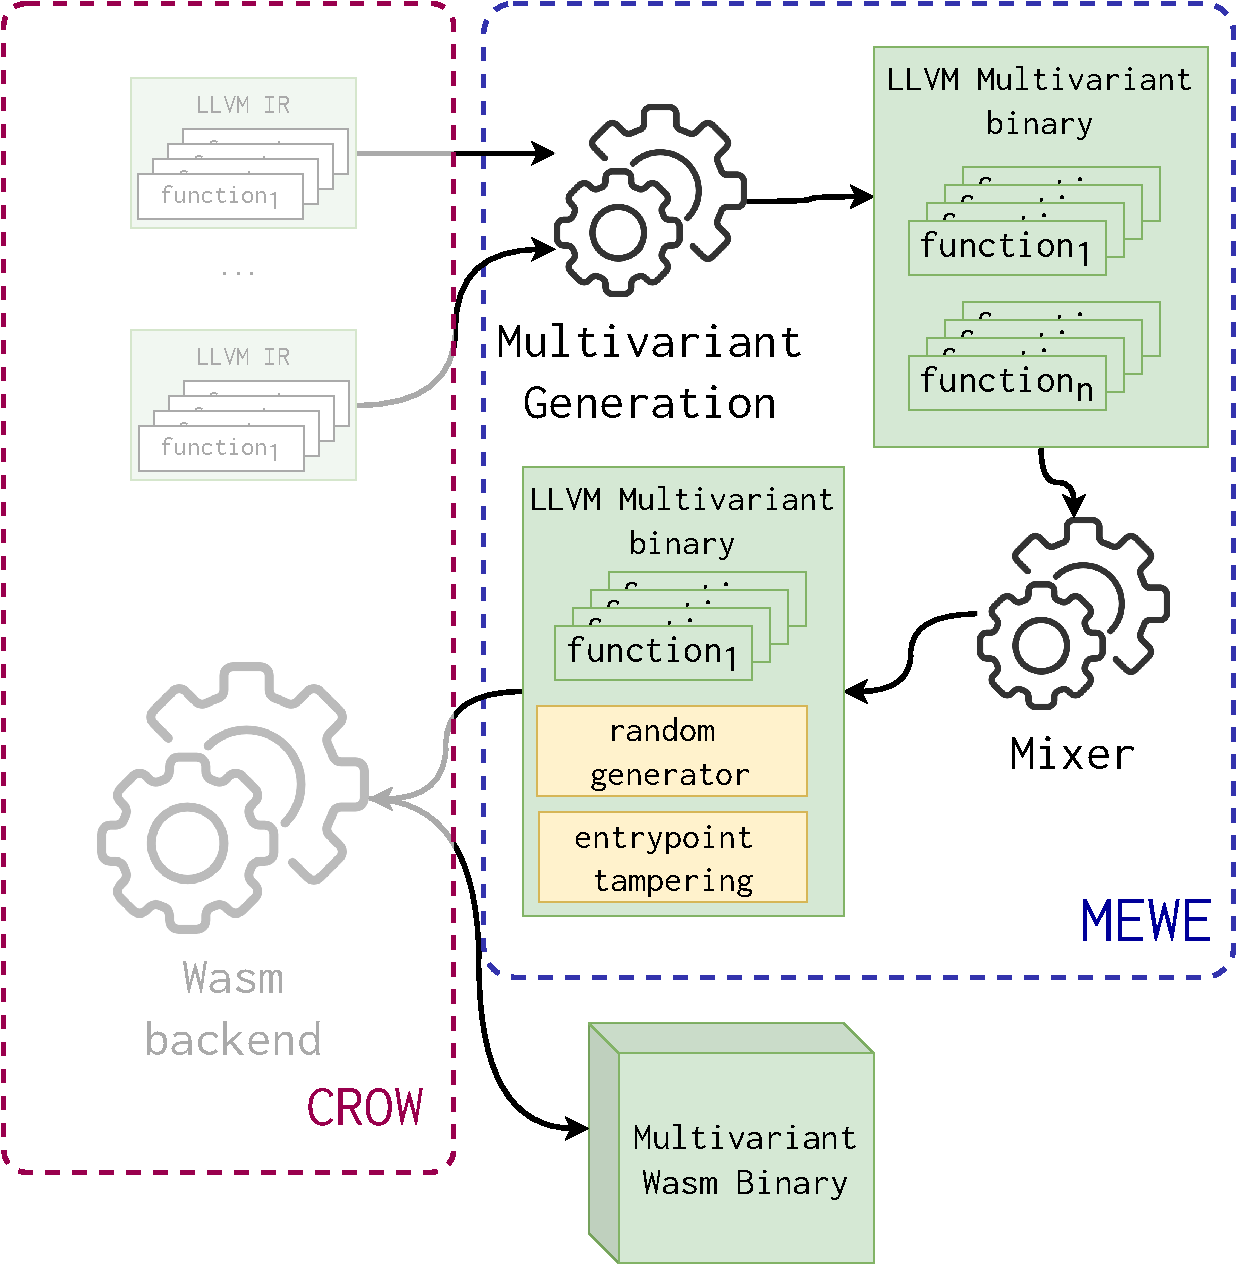
\includegraphics[height=3.2in]{diagrams/MEWE.pdf}
  \caption{Overview of \tool workflow. It takes as input an LLVM binary. It first generates a set of functionally equivalent variants for each function in the binary using CROW. Then, MEWE generates an LLVM multivariant binary composed of all the function variants. Finally, the Mixer includes the behavior in charge of selecting a variant when a function is invoked. Finally, the \tool mixer composes the LLVM multivariant binary with a random number generation library and tampers the original application entrypoint. The final process produces a \wasm\ multivariant binary ready to be deployed. }
  \label{workflow}
\end{figure*}


\msubsection{Multivariant generation}


The key component of \tool consists in combining the variants into a single binary.
The goal is to support execution-path randomization at runtime.
The core idea is to introduce one dispatcher function per original function with variants.
A dispatcher function is a synthetic function in charge of choosing a variant at random when the original function is called.
With the introduction of the dispatcher function,  \tool turns the original call graph into a multivariant call graph, defined as follows. 

\begin{definition}{Multivariant Call Graph (MCG):}\label{def:EP}
    A multivariant call graph is a call graph $\langle N, E \rangle$ where the nodes in $N$ represent all the functions in the binary and an edge $(f_1,f_2) \in E$ represents a possible invocation of $f_2$ by $f_1$  \cite{ryder1979}. The nodes in $N$ have three possible types: a function present in the original program,  a generated function variant, or a dispatcher function.
\end{definition}


\begin{figure}
    \centering
  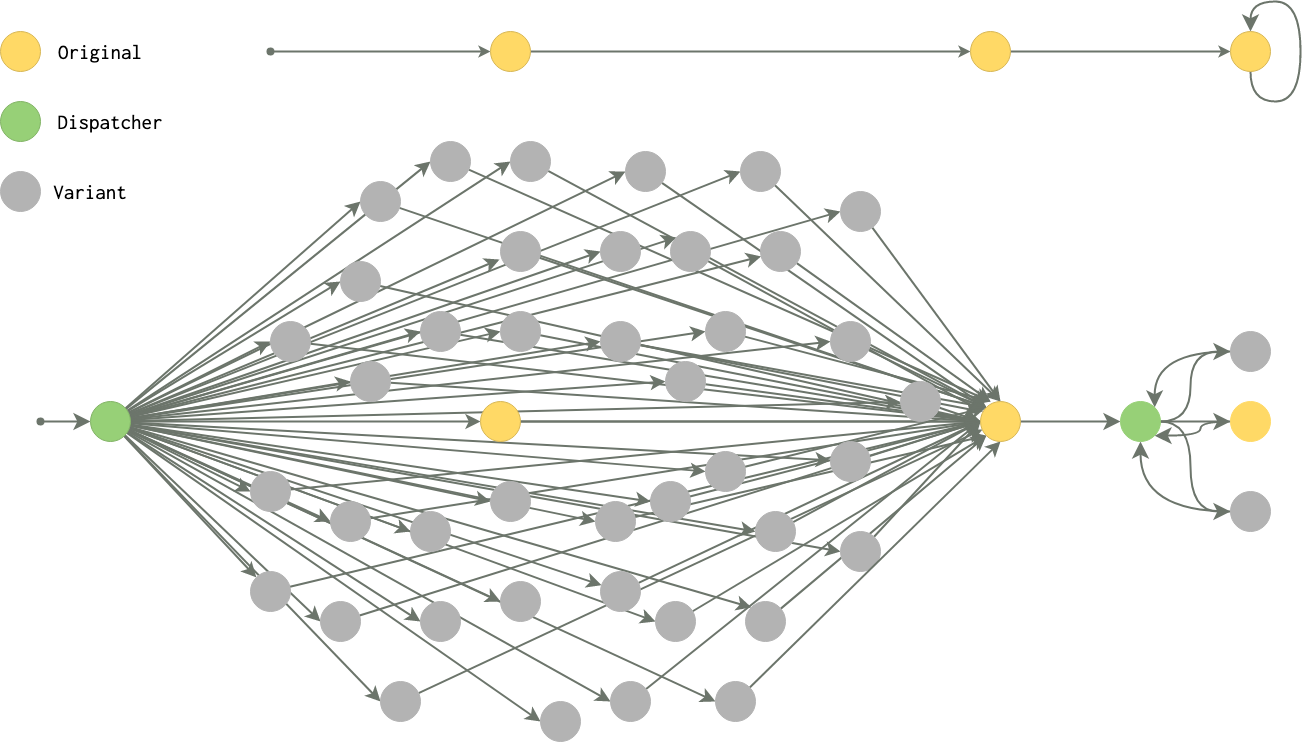
\includegraphics[width=.8\linewidth]{diagrams/CFG.png}
  \caption{Example of two static call graphs. At the top, the original call graph, at the bottom, the multivariant call graph, which includes nodes that represent function variants (in gray), dispatchers (in green), and original functions  (in yellow).
}
  \label{multivariant}
\end{figure}

% Instance of a multivariant module
In \autoref{multivariant}, we show the original static call graph for an original program (top of the figure), as well as the multivariant call graph generated with \tool (bottom of the figure).
The gray nodes represent function variants, the green nodes function dispatchers, and the yellow nodes are the original functions.
The directed edges represent the possible calls.
The original program includes three functions. \tool generates 43 variants for the first function, none for the second, and three for the third. 
\tool introduces two dispatcher nodes for the first and third functions. Each dispatcher is connected to the corresponding function variants to invoke one variant randomly at runtime.


% exaplanation of dispatcher
In  \autoref{listing:multivariant_template}, we illustrate the LLVM construction for the function dispatcher corresponding to the right most green node of \autoref{multivariant}.
It first calls the random generator, which returns a value used to invoke a specific function variant. 
We implement the dispatchers with a switch-case structure to avoid indirect calls that can be susceptible to speculative execution-based attacks \cite{Narayan2021Swivel}. 
The choice of a switch-case also avoids having multiple function definitions with the same signature, which could increase the attack surface in case the function signature is vulnerable \cite{johnson2021}.
This also allows \tool to inline function variants inside the dispatcher instead of defining them again.
Here we trade security over performance since dispatcher functions that perform indirect calls, instead of a switch-case,  could improve the performance of the dispatchers as indirect calls have constant time.
%It should be noted that the dispatcher function is constructed using the same signature as the original function. 


\lstset{
    language=llvm,
    %style=nccode,
    basicstyle=\footnotesize\ttfamily,
    columns=fullflexible,
    breaklines=true,
    numbers=none,
    stepnumber=1,
    float
}

\begin{code}
\scriptsize
\noindent\begin{minipage}[b]{\linewidth}
    \begin{minipage}[t]{1\linewidth}
        \begin{lstlisting}[escapeinside={(*}{*)}]
define internal i32 @foo(i32 %0) {
    entry:
      %1 = call i32 @discriminate(i32 3)
      switch i32 %1, label %end [
        i32 0, label %case_43_
        i32 1, label %case_44_
      ]
    case_43_:                 
      %2 = call i32 @foo_43_(%0)
      ret i32 %2
    case_44_:                
      %3 = <body of foo_44_ inlined>
      ret i32 %3
    end:                                             
      %4 = call i32 @foo_original(%0)
      ret i32 %4
}
        \end{lstlisting}
    \end{minipage}%
    
    \noindent\rule{\linewidth}{0.4pt}
    \captionof{lstlisting}{Dispatcher function embedded in the multivariant binary of the original function in the rightmost green node in \autoref{multivariant}.}\label{listing:multivariant_template}
\end{minipage}
\end{code}

\msubsection{The Mixer}

MEWE has four specific objectives: link the LLVM multivariant binary, inject a random generator, tamper the application's entrypoint, and merge all these components into a multivariant \wasm\ binary.
We use the Rustc compiler\footnote{\url{https://doc.rust-lang.org/rustc/what-is-rustc.html}} to orchestrate the mixing.
For the random generator, we rely on WASI's specification \cite{WASI} for the random behavior of the dispatchers. However, its exact implementation is dependent on the platform on which the binary is deployed.
The Mixer creates a new entrypoint for the binary called \emph{entrypoint tampering}.
It wraps the dispatcher for the entrypoint variants as a new function for the final Wasm binary and is declared as the application entrypoint. 

\msection{Binary based approach}

\msubsection{wasm-mutate}

%\subsection{CROW}
%\todo{Do not mentioend superoptimizers. Talk in terms of SMT encoding.}

%\subsection{Constant inferring}

%\subsection{Disabling optimisations}

%\subsection{MEWE}


%\section{Approaches comparison}

%\section{Accompanying artifacts}
\chapter{Assessing Software Diversification for \Wasm}
\label{exploit}



\chapterprecishere{If you find that you're spending all your time on theory, start turning some attention to practical things; it will improve your theories. If you find that you're spending almost all your time on practice, start turning some attention to theoretical things; it will improve your practice.\par\raggedleft--- {\small\textup{Donald Knuth}}}

\vspace{12mm}

\lettrine[lines=3]{I}{n} this chapter, we illustrate the application of Software Diversification for both offensive and defensive purposes.
We discuss two selected use cases that demonstrate the practical applications of our contributions.
Additionally, we discuss the challenges and benefits arising from the application of Software Diversification to \Wasm.





\msection{Offensive Diversification: Malware evasion}
\label{offensive_app}

The primary malicious use of WebAssembly in browsers is cryptojacking \cite{musch2019new}. 
This is due to the essence of cryptojacking, the faster the mining, the better. 
Let us illustrate how a malicious \Wasm binary is involved into browser cryptojacking.
\autoref{fig:attack_crypto} illustrates a browser attack scenario:
a practical WebAssembly cryptojacking attack consists of three components: a WebAssembly binary, a JavaScript wrapper, and a backend cryptominer pool. 
The WebAssembly binary is responsible for executing the hash calculations, which consume significant computational resources. 
The JavaScript wrapper facilitates the communication between the WebAssembly binary and the cryptominer pool.

\begin{figure}[h]
    \centering
    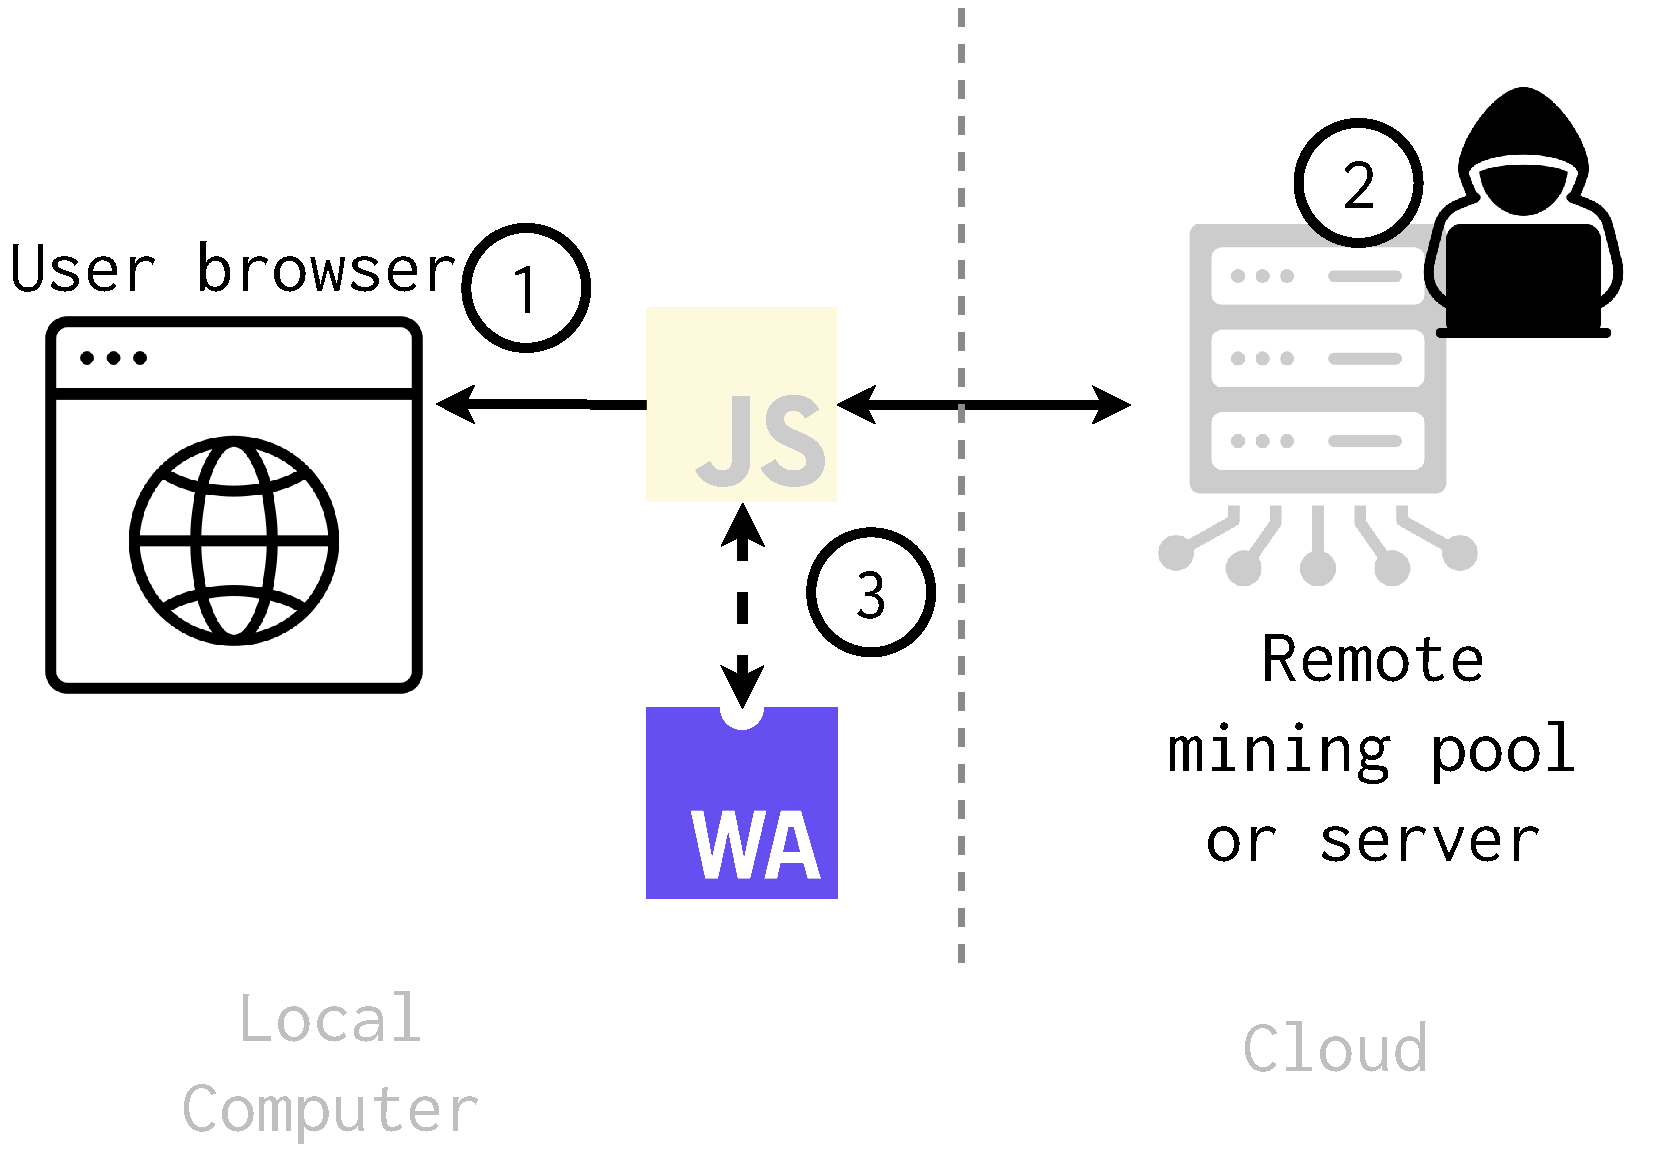
\includegraphics[width=0.6\linewidth]{figures/attack_crypto.pdf}
    \caption{A remote mining pool server, a JavaScript wrapper and the \Wasm binary form the triad of a cryptojacking attack in browser clients.}
    \label{fig:attack_crypto}
\end{figure}

The aforementioned components require the following steps to succeed in cryptomining.
First, the victim visits a web page infected with the cryptojacking code. 
The web page establishes a channel to the cryptominer pool, which then assigns a hashing job to the infected browser. 
The WebAssembly cryptominer calculates thousands of hashes inside the browser. 
Once the malware server receives acceptable hashes, it is rewarded with cryptocurrencies for the mining. 
Then, the server assigns a new job, and the mining process starts over.

Both antivirus software and browsers have implemented measures to detect cryptojacking. For instance, Firefox employs deny lists to detect cryptomining activities \cite{firefoxcrypto}. 
The academic community has also contributed to the body of work on detecting or preventing WebAssembly-based cryptojacking, as outlined in \autoref{background:wasm:analysis}. 
However, malicious actors can employ evasion techniques to circumvent these detection mechanisms. 
Bhansali \etal are among the first who have investigated how WebAssembly cryptojacking could potentially evade detection \cite{10.1145/3507657.3528560}, highlighting the critical importance of this use case. 
The case illustrated in the subsequent sections uses Offensive Software Diversification for evading malware detection in \Wasm. 

\msubsection{Cryptojacking defense evasion}
\label{threat_model}


Considering the previous scenario, several techniques can be directly implemented in browsers to thwart cryptojacking by identifying the malicious \Wasm components. 
Such defense scenario is illustrated in \autoref{fig:threat_model}, where the \Wasm malicious binary is blocked in \step{3}.
The primary aim of our use case is to investigate the effectiveness of code diversification as a means to circumvent cryptojacking defenses. 
Specifically, we assess whether the following evasion workflow can successfully bypass existing security measures:

\begin{figure}
    \centering
    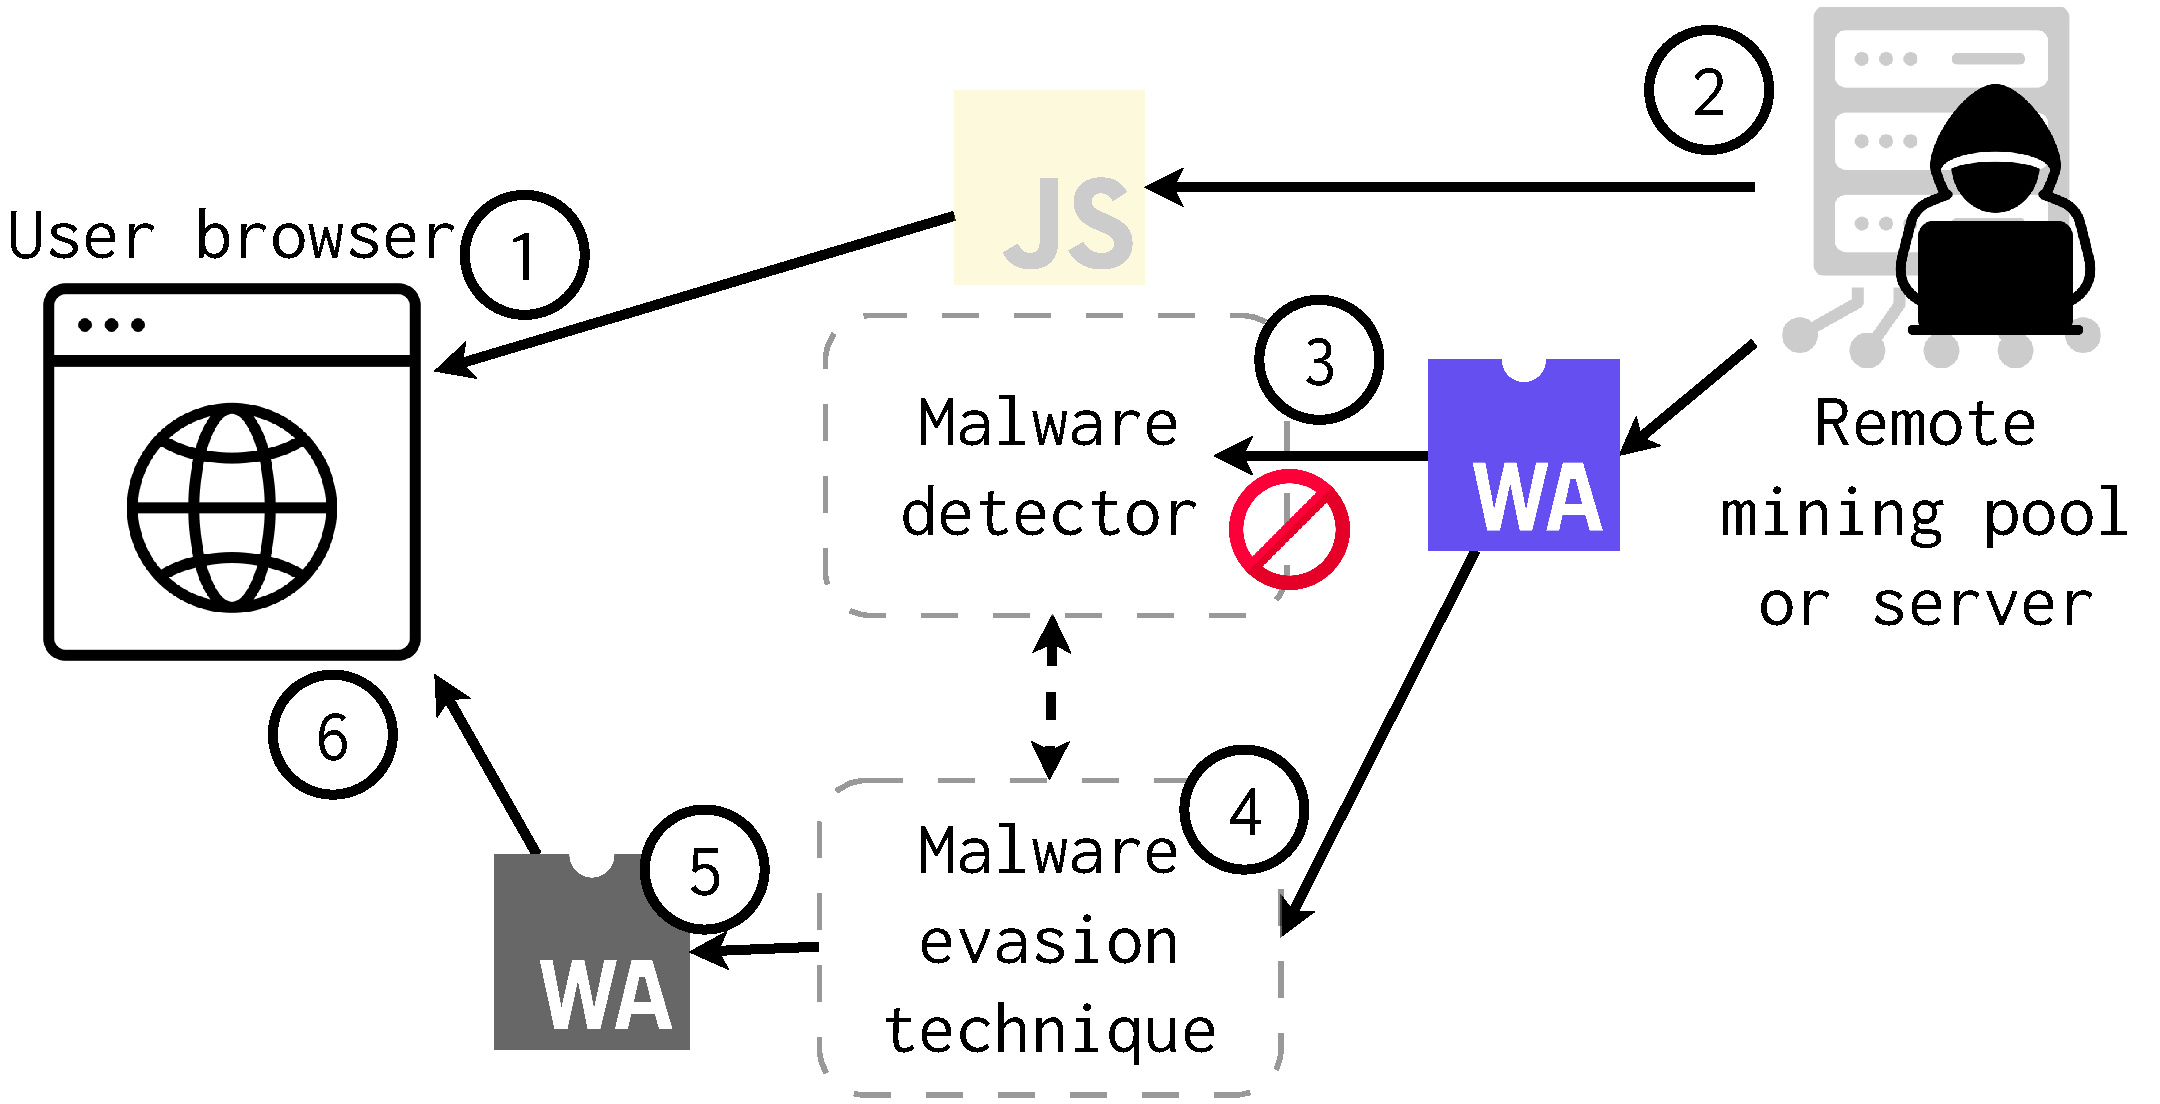
\includegraphics[width=0.8\linewidth]{figures/threat_model.pdf}
    \caption{Cryptojacking scenario in which the malware detection mechanism is bypassed by using an evasion technique.}
    \label{fig:threat_model}
\end{figure}


\begin{enumerate}
    
    \item The user loads a webpage infected with cryptojacking malware, which leverages network resources for execution—corresponding to \step{1} and \step{2} in \autoref{fig:threat_model}. 
    
    \item A malware detection mechanism (malware oracle) identifies and blocks malicious WebAssembly binaries at \step{3}. 
    For example, a network proxy could intercept and forward these resources to an external detection service via its API.
    
    \item Anticipating that a specific malware detection system is consistently used for defense, the attacker swiftly generates a variant of the WebAssembly cryptojacking malware designed to evade detection at \step{4}.
    
    \item The attacker delivers the modified binary instead of the original one \step{5}, which initiates the cryptojacking process and compromises the browser \step{6}. The detection method is not capable of detecting the malicious nature of the binary, and the attack is successful.
    
\end{enumerate}


\msubsection{Methodology}

Our aim is to validate, empirically, the effectiveness of Offensive Software Diversification in evading malware detection systems.
To achieve this, we employ WASM-MUTATE for generating \Wasm malware variants, with the goal of evading.
In this study, we categorize malware detection mechanisms as malware oracles, which can be of two types: binary and numeric. 
A binary oracle provides a binary decision, labeling a \Wasm binary as either malicious or benign. 
In contrast, a numeric oracle returns a numerical value representing the confidence level of the detection.

\begin{definition}{Malware oracle:}
    \label{malware_oracle_def}
    A malware oracle is a detection mechanism that returns either a binary decision or a numerical value indicating the confidence level of the detection.
\end{definition}


For empirical validation, we employ VirusTotal as a numeric oracle and MINOS \cite{MINOS} as a binary oracle. 
VirusTotal is an online service that analyzes files and returns a confidence score in the form of the number of antivirus that flag the input file as malware, thus qualifying as a numeric oracle. 
MINOS, on the other hand, converts \Wasm binaries into grayscale images and employs a convolutional neural network for classification. 
It returns a binary decision, making it a binary oracle.


We use the wasmbench dataset \cite{Hilbig2021AnES} to establish a ground truth. 
After running the wasmbench dataset through VirusTotal and MINOS, we identify 33 binaries that are: 1) flagged as malicious by at least one VirusTotal vendor and, 2) are also detected by MINOS.
Then, to simulate the evasion scenario, we use WASM-MUTATE to generate \Wasm binary variants to evade malware detection.
We use WASM-MUTATE in two configurations: controlled and stochastic diversification.

\begin{definition}{Feedback-guided Diversification:}
    \label{controlled_def}
    In feedback-guided diversification, the transformation process of a \Wasm program is guided by a numeric oracle, which influences the probability of each transformation. For instance, WASM-MUTATE can be configured to apply transformations that minimize the oracle's confidence score. Note that feedback-guided diversification needs a numeric oracle.
\end{definition}


\begin{definition}{Stochastic Diversification:}
    \label{uncontrolled_def}
    Unlike feedback-guided diversification, in stochastic diversification, each transformation has an equal likelihood of being applied to the input \Wasm binary.
\end{definition}


Based on the two types of malware oracles and diversification configurations, we examine three scenarios:
1) VirusTotal with a feedback-guided diversification, 2) VirusTotal with an stochastic diversification, and 3) MINOS with a stochastic diversification.
Notice that, the fourth scenario with MINOS and a feedback-guided diversification is not feasible, as MINOS is a binary oracle and cannot provide the numerical values required for feedback-guided diversification.

Our evaluation focuses on three key metrics: the success rate of evading detection mechanisms in VirusTotal and MINOS across the 33 flagged binaries, the correctness of the generated variants, and the performance impact on the variants that successfully evade detection.
The first metric measures the efficacy of WASM-MUTATE in bypassing malware detection systems. 
For each flagged binary, we input it into WASM-MUTATE, configured with the selected oracle and diversification strategy. 
We then iteratively apply transformations to the output from the preceding step. 
This iterative process is halted either when the binary is no longer flagged by the oracle or when a maximum of 1000 stacked transformations have been applied (see \autoref{stack_transform}).
This process is repeated with 10 random seeds per binary to simulate 10 different evasion experiments per binary.
The second metric is crucial for validating the real-world applicability of WASM-MUTATE in evading malware detection. 
Specifically, if the evasion process significantly degrades the performance of the resulting binary compared to its original version, it becomes less likely to be employed in practical scenarios, such as cryptojacking.
For this, we execute, end-to-end, the variants that fully evade VirusTotal when generated with WASM-MUTATE in controlled and stochastic diversification configurations.
We select variants for which we could completely reproduce the three components in \autoref{fig:attack_crypto}.

\msubsection{Results}

In \autoref{offensive:results:fast}, we present a comprehensive summary of the evasion experiments presented in \cite{EVASION}, focusing on two oracles: VirusTotal and MINOS\cite{MINOS}. 
The table is organized into two main categories to separate the results for each malware oracle. 
For VirusTotal, we further subdivide the results based on the two diversification configurations we employ: stochastic and feedback-guided diversification. 
In these subsections, the columns indicate the number of VirusTotal vendors that flag the original binary as malware (\#D), the maximum number of successfully evaded detectors (Max. \#evaded), and the average number of transformations required (Mean \#trans.) for each sample. 
We highlight in bold text the values for which the stochastic diversification or feedback-guided diversification setups best, the lower, the better.
The MINOS section solely includes a column that specifies the number of transformations needed for complete evasion. 
The table has 33 + 1 rows, each representing a unique \Wasm malware study subject. 
The final row offers the median number of transformations required for evasion across our evaluated setups and oracles. 

\newcolumntype{t}{>{\columncolor{Gray}}r}
\begin{table}
    \footnotesize
    \centering
    \begin{tabular}{c | r | r l | r l | t }
        \hline
        & \multicolumn{5}{|c|}{VirusTotal} & MINOS\cite{MINOS} \\
        \hline
        Hash & \#D & \multicolumn{2}{c|}{Stochastic diversification} & \multicolumn{2}{c|}{Feedback-guided diversification} & \\
        \hline
        &  & Max. #evaded & Mean #trans. & Max. #evaded & Mean #trans. & Mean #trans. \\
        \hline\hlined
        47d29959 &                 31 &             \textbf{26} &     N/A & 19 & N/A  & 100  \\ 
        9d30e7f0 &                 30 &             \textbf{24}  &      N/A & 17 & N/A & 419  \\ 
        8ebf4e44 &                 26 &             \textbf{21} &     N/A  & 13 & N/A & 92 \\
        \hline
        c11d82d &                 20 &       20        &  \textbf{355} & 20 & 446 & 115 \\ 
        0d996462 &                 19 &     19    &  \textbf{401} & 19 & 697 & 24 \\ 
        a32a6f4b &                 18 &       18       &  635 & 18 & \textbf{625} & 1 \\
        
        
        fbdd1efa &                 18 &         18      &  \textbf{310} & 18 & 726 & 1 \\ 
        d2141ff2 &                  9 &          9      &  \textbf{461} & 9 & 781 & 81 \\ 
        aafff587 &                  6 &          6      &  484 & 6 & \textbf{331} & 1 \\
        
        
        046dc081 &                  6 &          6      &  404 & 6 & \textbf{159} & 33 \\ 
        643116ff &                  6 &          6      &  \textbf{144} & 6 & 436 & 47 \\ 
        15b86a25 &                  4 &          4      &  253 & 4 & \textbf{131} & 1 \\
        
        
        
        006b2fb6 &                  4 &           4     &  \textbf{282} & 4 & 380 & 1\\ 
        942be4f7 &                  4 &           4     &  200 & 4 & 200 & 29\\ 
        7c36f462 &                  4 &           4     &  236 & 4 & \textbf{221} & 85\\
        
        
        fb15929f &                  4 &            4    &  \textbf{297} & 4 & 475 & 1 \\ 
        24aae13a &                  4 &         4       &  \textbf{252 } & 4 & 401 & 980\\ 
        000415b2 &                  3 &         3       &  302 & 3 & \textbf{34} & 960 \\
        
        4cbdbbb1 &                  3 &          3      &  295 & 3 & \textbf{72} & 1\\ 
        65debcbe &                  2 &          2      &  131  & 2 & \textbf{33} & 38 \\ 
        59955b4c &                  2 &          2      &  130  & 2 & \textbf{33} & 38 \\
        
        
        89a3645c &                  2 &           2     &  431 & 2 & \textbf{107} & 108\\
        a74a7cb8 &                  2 &           2     &  124 & 2 & \textbf{33} & 38 \\
        119c53eb &                  2 &           2     &  104 & 2 & \textbf{18} & 1 \\
        
        089dd312 &                  2 &           2     &  153 & 2 & \textbf{123} & 68\\
        c1be4071 &                  2 &           2     &  130 & 2 & \textbf{33} & 38\\
        dceaf65b &                  2 &           2     &  140 & 2 & 132 & 66\\
        
        6b8c7899 &                  2 &            2    &  143 & 2 & \textbf{33} & 38 \\
        a27b45ef &                  2 &         2       &  145 & 2 & \textbf{33} & 33\\
        68ca7c0e &                  2 &         2       &  137  & 2 & \textbf{33} & 38\\
        
        f0b24409 &                  2 &         2       &  127  & 2 & \textbf{11} & 33 \\
        5bc53343 &                  2 &         2       &  118  & 2 & \textbf{33} & 33 \\
        e09c32c5 &                  1 &         1       &  \textbf{120}  & 1 & 488 & 15 \\
        \hline\hline
        Median &                         &         &      218  &   & 131 & 38
    \end{tabular}
    \caption{
        The table has two main categories for each malware oracle, corresponding to the two oracles we use: VirusTotal and MINOS. 
        For VirusTotal, divide the results based on the two diversification configurations: stochastic and feedback-guided diversification. 
        We provide columns that indicate the number of VirusTotal vendors that flag the original binary as malware (\#D), the maximum number of successfully evaded detectors (Max. \#evaded), and the average number of transformations required (Mean \#trans.) for each sample. 
        We highlight in bold text the values for which diversification setups are best, the lower, the better.
        The MINOS section includes a column that specifies the number of transformations needed for complete evasion. 
        The final row offers the median number of transformations required for evasion across our evaluated setups and oracles. 
    }
    \label{offensive:results:fast}
\end{table}

\begin{strategy}[Stochastic diversification to evade VirusTotal]
    \label{stochastic_div_vt}
    We execute a stochastic diversification with WASM-MUTATE, setting a limit of 1000 iterations for each binary. 
    In every iteration, we query VirusTotal to determine if the newly generated binary can elude detection. 
    We repeat this procedure with ten distinct seeds for each binary, replicating ten different evasion experiments. 
    As the stochastic diversification section of \autoref{offensive:results:fast} illustrates, we successfully produce variants that fully evade detection for 30 out of 33 binaries. 
    The average amount of iterations required to produce a variant that evades all detectors oscillates between 120 to 635 stacked transformations. 
    The mean number of iterations needed never exceeds 1000 stacked transformations. 
    However, three binaries remain detectable under the stochastic diversification setup. 
    In these instances, the algorithm fails to evade 5 out of 31, 6 out of 30, and 5 out of 26 detectors. 
    This shortfall can be attributed to the maximum number of iterations, 1000, that we employ in our experiments. 
    Increasing iterations further, however, seems unrealistic. 
    If certain transformations enlarge the binary size, a significantly large binary could become impractical due to bandwidth limitations. 
    In summary, stochastic diversification with WASM-MUTATE markedly reduces the detection rate by VirusTotal antivirus vendors for cryptojacking malware, achieving total evasion in 30 out of 33 (90\%) cases within the malware dataset. 
    %WASM-MUTATE proves capable of successfully evading detection systems in just a few minutes.    
\end{strategy}
    

\begin{strategy}[Feedback-guided diversification to evade VirusTotal]
    \label{guided_div_vt}
    stochastic diversification does not guide the diversification based on the number of evaded detectors, it is purely random, and has some drawbacks.
    For example, some transformations might suppress other transformations previously applied.
    We have observed that, by carefully selecting the order and type of transformations applied, it is possible to evade detection systems in fewer iterations.
    This can be appreciated in the results of the feedback-guided diversification part of \autoref{offensive:results:fast}.
    The feedback-guided diversification setup successfully generates variants that totally evade the detection for 30 out of 33 binaries, it is thus as good as the stochastic setup.
    Remarkably, for 21 binaries out of 30, feedback-guided needs only 40\% of the calls the stochastic diversification setup needs, demonstrating larger efficiency. 

    %In practice, a potential attacker may be limited by budget on the number of transformations applicable to the malware binary, e.g., the number of queries to VirusTotal. 
    %Additionally, the performance of the resulting binary benefits from this approach.

\end{strategy}
  
\begin{strategy}[Stochastic diversification to evade MINOS]
    \label{stochastic_div_minos}
    Relying exclusively on VirusTotal for detection could pose issues, particularly given the existence of specialized solutions for \Wasm, which differ from the general-purpose vendors within VirusTotal. 
    In \autoref{background:wasm:analysis} we highlight several examples of such solutions.
    Yet, for its simplicity, we extend this experiment by using MINOS\cite{MINOS}, an antivirus specifically designed for \Wasm. 
    The results of evading MINOS can be seen in the final column of \autoref{offensive:results:fast}.
    The bottom row of \autoref{offensive:results:fast} highlights that fewer iterations are required to evade MINOS than VirusTotal through WebAssembly diversification, indicating a greater ease in eluding MINOS.
    The stochastic diversification setup requires a median iteration count of 218 to evade VirusTotal. 
    In contrast, the feedback-guided diversification setup necessitates only 131 iterations. 
    Remarkably, a mere 38 iterations are needed for MINOS. 
    In tests against MINOS, WASM-MUTATE evaded detection for 8 out of 33 binaries in a single iteration. 
    This result implies a vulnerability in the MINOS model to binary diversification.
\end{strategy}

\begin{strategy}[Meta-oracles]
    \label{meta-oracles}
    Our experiments indicate that VirusTotal surpasses MINOS in detecting \Wasm cryptojacking. 
    The primary factor contributing to this is VirusTotal's utilization of a broader range of antivirus vendors, which employs various detection strategies. 
    On the other hand, MINOS functions as a binary oracle. 
    This evidence supports the use of multiple malware oracles (meta-oracles) in identifying cryptojacking malware in browsers. 
    In the context of \Wasm, given the existence of numerous and diverse Wasm-specific detection mechanisms, this strategy is both practical and feasible, yet not explored in the literature.
\end{strategy}
    
%\msubsection{Efficiency and correctness results}

\begin{strategy}[\Wasm variants correctness]
    \label{evasion_impact}
    To evaluate the correctness of the malware variants created with WASM-MUTATE, we focused on six binaries that we could build and execute end-to-end, as these had all three components outlined in \autoref{fig:attack_crypto}. 
    We select only six binaries because the process of building and executing the binaries involves three components. 
    As detailed in \autoref{fig:attack_crypto}, they include the \Was binary, its JavaScript complement, and the miner pool. 
    These components were not found for the remaining 24 evaded binaries in the study subjects.
    For the six binaries, we then replace the original WebAssembly code with variants generated using VirusTotal as the malware oracle and WASM-MUTATE for both controlled and stochastic diversification configurations. 
    We then execute both the original and the generated variants. 
    We assess the correctness of the variants by examining the hashes they generate.
    If a minerpool detects a variant's generated hash as incorrect, or if the variant crashes during execution, we conclude an incorrect variant is created.
    Our findings show that all variants generated with WASM-MUTATE are correct, i.e., they generate the correct hashes and execute without error.
    Additionally, we found that 19\% of the generated variants surpassed the original cryptojacking binaries in performance.
\end{strategy}

\begin{tcolorbox}[title=Contribution paper,boxrule=1pt,arc=.2em,boxsep=1.0mm]
    WASM-MUTATE generates correct and performant variants of WebAssembly cryptojacking that successfully evade malware detection.
    The case discussed in this section is fully detailed in Cabrera-Arteaga \etal "WebAssembly Diversification for Malware Evasion"
    \emph{at Computers \& Security, 2023}
    \url{https://www.sciencedirect.com/science/article/pii/S0167404823002067}. 
\end{tcolorbox}


% Efficiency
%We have found that 
%This improvement is attributed to WASM-MUTATE's ability to introduce code optimizations. 
%Additionally, debloating transformations, which eliminate unnecessary structures and dead code, resulted in a higher hash generation rate during the initial seconds of mining, likely due to faster compilation times. 
%This suggests that focused optimization serves as a valuable tool for evasion in browsers.
% The contrary case.
%On the contrary, 80\% of the generated variants are less efficient than the original binary, with the least efficient variant operating at only 20\% of the original hash generation rate. 
%This performance drop is primarily due to non-optimal transformations introduced by WASM-MUTATE. 
%Variants generated through stochastic diversification are generally slower.
%In summary, feedback-guided diversification yielded variants that evaded VirusTotal detection with minimal performance overhead—the worst-performing variant was only 1.93 times slower than the original.


\msection{Defensive Diversification: Speculative Side-channel protection}

As previously discussed in \autoref{background:wasm:ecosystems}, \Wasm is rapidly gaining traction in backend environments. 
Companies like Cloudflare and Fastly are encouraging the use of \Wasm in their edge computing platforms, allowing developers to deploy faster applications in a modular and securely sandboxed fashion. 
Typically, these client \Wasm applications are designed as isolated services with a single, focused responsibility.
This model is usually called Function-as-a-Service (FaaS) \cite{pMendkiServerless, 1244493Jacobsson}.

The core concept behind \wasm in FaaS platforms is the ability to host thousands of client \Wasm binaries within a single host process, which is then distributed across multiple servers and data centers. 
To achieve this, the platforms compile the \wasm programs to native code, which is then executed in a sandboxed environment.
Then, the host processes are capable of instantiating a new Wasm sandbox for each client function, executing it in response to individual user requests in a matter of nanoseconds. 
Utilizing \Wasm enables these platforms to inherently isolate the execution of client functions from one another as well as from the host process.
However, this isolation is not foolproof against Spectre attacks \cite{Spectre,Narayan2021Swivel}.


In the subsequent sections, we illustrate how diversification can be used to protect \Wasm binaries against Spectre attacks.
We show a case of Defensive Software Diversification for the sake of protecting \Wasm binaries. 

\msubsection{Threat model: speculative side-channel attacks}

Let us illustrate the threat model in which a \Wasm program could be susceptible in FaaS platforms.
Developers can submit any \Wasm binary to the FaaS platform.
This includes potential malicious actors that could upload a \wasm binary that, when compiled to native code, uses Spectre attacks to leak sensitive information from the host process.
Spectre attacks exploit hardware predictors to induce misspredictions and speculatively execute instructions—gadgets that would not run sequentially. 
The attacker could then use this information to infer the contents of the memory of other client functions, or even the host process itself.

Narayan and colleagues \cite{Narayan2021Swivel} dissected the possible Spectre attacks for \wasm binaries into three categories based on the specific hardware predictor that is exploited and the specific FaaS scenario: Sandbox breakout attacks, Sandbox poisoning attacks and Host poisoning attacks.
The first one, exploits the branch target buffer by predicting the target of an indirect jump, thereby rerouting speculative control flow to an arbitrary target.
The second one takes advantage of the pattern history table to anticipate the direction of a conditional branch during the ongoing evaluation of a condition.
The third and last one exploits the return stack buffer that stores the locations of recently executed call instructions to predict the target of \texttt{ret} instructions. 
Each attack methodology relies on the extraction of memory bytes from another hosted \wasm binary that executes in the same host process.



\todo{Add diagram}
\todo{Explain here the threat model with the diagram}

%\lipsum[1]

%\lipsum[1]

\msubsection{Approach}
%\lipsum[1]

- Use of wasm-mutate

\msubsection{Results}

- Diminshing of BER
- Rockiki paper on portable side channel in browsers.



\todo{TBD discuss deoptimization}
% \subsection{Deoptimization}

\subsection{Partial input/output validation}

% We need to talk about this because, we do this checking right noe and it is probably a reason for the low count of variants.
When \tool generates a variant, it can be executed to check the input/output equivalence.
If the variant has a \_start function, both binaries, the original and the variant can be initialized. 
If the state of the memory, the globals and the stack is the same after executing the \_start function, they are partially equivalent.
%This mechanismm is already implemented in the fuzzing campaign of wasmtime.

The \_start function is easier to execute given its signature.
It does not receive parameters.
Therefore, it can be executed directly.
Yet, since a \Wasm program might contain more than one function that could be indistinctly called with and arbitrary number of parameters, we are not able to validate the whole program.
Thus, we call the checking of the initialization of a \wasm variant, a partial validation.

\subsection{Some other works to be cited along with the paper. Mostly in the Intro}

\emph{Spectre and side-channel defenses}

- paper 2021: Read this, since it is super related, \url{https://www.isecure-journal.com/article_136367_a3948a522c7c59c65b65fa87571fde7b.pdf} \cite{WasmSpectre}


- A dataset of Wasm programs: \cite{nicholson2023wasmizer}

- Papers 2020

- Papers 2019
- \cite{10.1145/3510003.3510070}

Selwasm: A code protection mechanism for webassembly


Babble

- https://arxiv.org/pdf/2212.04596.pdf

Principled Composition of Function Variants for Dynamic
Software Diversity and Program Protection

- https://dl.acm.org/doi/10.1145/3551349.3559553

How Far We’ve Come – A Characterization Study of Standalone WebAssembly Runtimes

- https://ieeexplore.ieee.org/document/9975423

Code obfuscation against symbolic execution attacks

Code artificiality: A metric for the code stealth based on an n-gram model

Semantics-aware obfuscation scheme prediction for binary

Wobfuscator: Obfuscating javascript malware via opportunistic translation to webassembly

Synthesizing Instruction Selection Rewrite Rules from RTL using SMT
"We also synthesize integer rewrite rules from WebAssembly to RISC-V "

Wafl: Binary-only webassembly fuzzing with fast snapshots



\begin{tcolorbox}[title=Contribution paper,boxrule=1pt,arc=.2em,boxsep=1.0mm]
    The case discussed in this section is fully detailed in Cabrera-Arteaga \etal "WASM-MUTATE: Fast and Effective Binary Diversification for WebAssembly"
    \emph{Under review}
    \url{https://arxiv.org/pdf/2309.07638.pdf}. 
\end{tcolorbox}




\msection{Intrinsic properties of diversification}
\label{exploit:discussion}
In \autoref{exploit:defensive}, we have noted an increasing trend of exfiltration bandwidth in certain variants. 
\autoref{offensive_app} presents a similar case, indicating that without a clear objective in the diversification process, uncontrolled diversification can be counterproductive. 
This implies that not all transformations contribute equally to the diversification objectives of \Wasm.
In the following, we elaborate on three cornerstones properties for improving Software Diversification with relation to \Wasm.

\wrule{Preservation:}
Some transformations yield distinct \Wasm binaries, yet their JIT compilation produces identical machine code.
Non-preserved transformations undermine the effectiveness of diversification, as discussed in \autoref{discussion}.
Incorporating random \texttt{nop} operations directly into \Wasm, for instance, does not alter the final machine code because JIT compilers typically eliminate these \texttt{nop} operations.
This phenomenon is also observed with transformations to the custom sections of \Wasm binaries.
Identical machine code, even when their \Wasm variants are different, can be detected by malware detectors.
For practitioners, malware detection tools can be enhanced by incorporating a pre-compilation step to normalize \Wasm binaries.
Besides, developers could focus on transformations that preserve the machine code, as they are more likely to contribute to the diversification objectives, e.g., evasion.
On the other hand, side-channel attacks occur at the machine code level.
Thus, making \Wasm variants preservation is essential code for successful defensive diversification, i.e., if the machine code is preserved, the side-channel attack will not be effective against the \Wasm variant.


%\wrule{Dead code addition:} 
%Transformed code may not always execute. 
%For example, Software Diversification might generate dead code or introduce a new function that the original program does not execute. 
%This is beneficial for static analysis, whether for avoiding reverse engineering or proving static malware detection. 
%However, dynamic analysis tools can identify this type of variant, e.g., this might reduce the effectiveness of evasion. 
%Furthermore, the inclusion of non-executing dead code does not affect side-channels.
%When the variant executes, it behaves identically to the original program, thereby not strengthening against potential attacks.
 
% More fine grained
\wrule{Disrupting timers:} Cache timing side-channel attacks, including for the four binaries analyzed in \autoref{exploit:defensive}, depend on precise timers to measure cache access times. 
Disrupting these timers can effectively neutralize the attack \cite{JStimers}. 
The \Wasm variants inherently adopt a similar approach, introducing perturbations in the timing steps of \Wasm variants. 
This is illustrated in \autoref{example:timer} and \autoref{example:timer2}, where the former shows the original time measurement and the latter presents a variant with introduced operations.
By introducing additional instructions, the inherent randomness in the time measurement of a single or a few instructions is amplified, thereby reducing the timer's accuracy. 


\lstdefinestyle{watcode}{
  numbers=none,
  stepnumber=1,
  numbersep=10pt,
  tabsize=4,
  showspaces=false,
  breaklines=true, 
  showstringspaces=false,
    moredelim=**[is][{\btHL[fill=weborange!40]}]{`}{`},
    moredelim=**[is][{\btHL[fill=celadon!40]}]{!}{!}
}


   \begin{minipage}[b]{\linewidth}
    \lstset{
        language=WAT,
                        style=watcode,
        basicstyle=\footnotesize\ttfamily,
                        columns=fullflexible,
                        breaklines=true}
        
        \begin{lstlisting}[label=example:timer,caption={Wasm timer code.},frame=b, captionpos=b]{Name}
;; Code from original btb_breakout
...
(call $readTimer)
(set_local $end_time)
... access to mem
(i64.sub (get_local $end_time ) (get_local $start_time))
(set_local $duration)
...

        \end{lstlisting}
\end{minipage}


\begin{minipage}[b]{\linewidth}
    \lstset{
        language=WAT,
                        style=watcode,
        basicstyle=\footnotesize\ttfamily,
                        columns=fullflexible,
                        breaklines=true}
        
        \begin{lstlisting}[label=example:timer2,caption={\Wasm variant with more instructions added in between time measurement.},frame=b, captionpos=b]{Name}
;; Variant code
...
(call $readTimer)
(set_local $end_time)
!<inserted instructions>!
... access to mem
!<inserted instructions>!
(i64.sub (get_local $end_time ) (get_local $start_time))
(set_local $duration)
...
        \end{lstlisting}
\end{minipage}


\todo{Recheck term-citation padding here}

\wrule{Padding speculated instructions:} CPUs have a limit on the number of instructions they can cache. 
Diversification injects instructions to potentially exceed this limit, effectively disabling the speculative execution of memory accesses. 
This approach is akin to padding \cite{padding}, as demonstrated in \autoref{example:padding} and \autoref{example:padding2}.
This padding disrupts the binary code's layout in memory, hindering the attacker's ability to initiate speculative execution. 
Even if speculative execution occurs, the memory access does not proceed as the attacker intended.


\lstdefinestyle{watcode}{
  numbers=none,
  stepnumber=1,
  numbersep=10pt,
  tabsize=4,
  showspaces=false,
  breaklines=true, 
  showstringspaces=false,
    moredelim=**[is][{\btHL[fill=weborange!40]}]{`}{`},
    moredelim=**[is][{\btHL[fill=celadon!40]}]{!}{!}
}


   \begin{minipage}[b]{0.8\linewidth}
    \lstset{
        language=WAT,
                        style=watcode,
        basicstyle=\footnotesize\ttfamily,
                        columns=fullflexible,
                        breaklines=true}
        
        \begin{lstlisting}[label=example:padding,caption={Two jump locations. The top one trains the branch predictor, the bottom one is the expected jump that exfiltrates the memory access.},frame=b, captionpos=b]{Name}
;; Code from original btb_breakout
...
;; train the code to jump here (index 1)
(i32.load (i32.const 2000))
(i32.store (i32.const 83)) ;; just prevent optimization
...
;; transiently jump here
(i32.load (i32.const 339968)) ;; S(83) is the secret
(i32.store (i32.const 83)) ;; just prevent optimization
        \end{lstlisting}
\end{minipage}


\begin{minipage}[b]{0.8\linewidth}
    \lstset{
        language=WAT,
                        style=watcode,
        basicstyle=\footnotesize\ttfamily,
                        columns=fullflexible,
                        breaklines=true}
        
        \begin{lstlisting}[label=example:padding2,caption={\Wasm variant with more instructions added indindinctly between jump places.},frame=b, captionpos=b]{Name}
;; Variant code
...
;; train the code to jump here (index 1)
!<inserted instructions>!
(i32.load (i32.const 2000))
!<inserted instructions>!
(i32.store (i32.const 83)) ;; just prevent optimization
...
;; transiently jump here
!<inserted instructions>!
(i32.load (i32.const 339968)) ;; "S"(83) is the secret
!<inserted instructions>!
(i32.store (i32.const 83)) ;; just prevent optimization
...
        \end{lstlisting}
\end{minipage}






% \msection{Threats to validity}
\label{threats}

We discuss the threats to the validity of the two use cases presented in this chapter.
We separate the threats to validity into three main categories: internal, external, and construct validity.

\msubsection{Internal validity}


\msubsection{External validity}


\msubsection{Construct validity}


\subsection{Partial input/output validation}

% We need to talk about this because, we do this checking right noe and it is probably a reason for the low count of variants.
When \tool generates a variant, it can be executed to check the input/output equivalence.
If the variant has a \_start function, both binaries, the original and the variant can be initialized. 
If the state of the memory, the globals and the stack is the same after executing the \_start function, they are partially equivalent.
%This mechanismm is already implemented in the fuzzing campaign of wasmtime.

The \_start function is easier to execute given its signature.
It does not receive parameters.
Therefore, it can be executed directly.
Yet, since a \Wasm program might contain more than one function that could be indistinctly called with and arbitrary number of parameters, we are not able to validate the whole program.
Thus, we call the checking of the initialization of a \wasm variant, a partial validation.


\section{Conclusions}
In this chapter, we explore Offensive and Defensive Software Diversification applied to \Wasm.
Offensive Software Diversification highlights both the potential and the latent security risks in applying Software Diversification to \Wasm malware. 
Our findings suggest potential enhancements to the automatic detection of cryptojacking malware in WebAssembly, e.g., by stressing their resilience with \Wasm malware variants. 
Conversely, Defensive Software Diversification serves as a proactive guard, specifically designed to mitigate the risks associated with Spectre attacks. 

Moreover, we have conducted experiments with various use cases that are not shown in this chapter.
For instance, CROW \cite{CROW} excels in generating \Wasm variants that minimize side-channel noise, thereby bolstering defenses against potential side-channel attacks. 
Alternatively, deploying multivariants from MEWE \cite{MEWE} can thwart high-level timing-based side-channels \cite{morgan2015web}. 
Specifically, we conducted experiments on the round-trip times of the generated multivariants and concluded that, at a high level, the timing side-channel information cannot discriminate between variants. 


\chapter{Conclusions and Future Work}
\label{results}

%\lipsum[1]

\section{Summary of technical contributions}

%\lipsum[1]

%\lipsum[2]

%\lipsum[3]

\section{Summary of empirical findings}

%\lipsum[1]

%\lipsum[1]

%\lipsum[1]

\section{Future Work}

%\lipsum[1]

Moreover, the \Wasm ecosystem is still in its infancy compared to more mature programming environments. 
A 2021 study by Hilbig et al. found only 8,000 unique \Wasm binaries globally\cite{Hilbig2021AnES}, a fraction of the 1.5 million and 1.7 million packages available in npm and PyPI, respectively. 
This limited dataset poses challenges for machine learning-based analysis tools, which require extensive data for effective training. 
The scarcity of \Wasm programs also exacerbates the problem of software monoculture, increasing the risk of compromised \Wasm programs being consumed\cite{usenixWasm2020}. 
This dissertation aims to mitigate these issues by introducing a comprehensive suite of tools designed to enhance \Wasm security through Software Diversification and to improve testing rigor within the ecosystem.


\emph{Program Normalization}
\tool was previously employed successfully for the evasion of malware detection, as outlined in \cite{CABRERAARTEAGA2023103296}. 
The proposed mitigation in the prior study involved code normalization as a means of reducing the spectrum of malware variants. 
Our current work provides insights into the potential effectiveness of this approach. 
Specifically, a practically costless process of pre-compiling Wasm binaries could be employed as a preparatory measure for malware classifiers. 
In other words, a \wasm binary can first be compiled with wasmtime, effectively eliminating approx. 25\% of malware variants according to our preservation statistics for wasmtime. 
This approach could substantially enhance the efficiency and precision of malware detection systems.


%\lipsum[1]
%\chapter{Conclusions and Future Work}
\label{conclusions}


%------------------------------------------------
% CREATING THE BIBLIOGRAPHY
%------------------------------------------------
\bibliographystyle{ieeetr}
\renewcommand{\bibname}{References}% changes default name Bibliography to References
\bibliography{Kappa} % References file

%--------------------------------------------------
%\addcontentsline{toc}{chapter}{Appended papers} % for template purposes
\part{Included papers}
\stepcounter{page} % Skip the current page

% Each chapter is a paper
% chapter tiltes formatting
\titleformat{\chapter}[display]
  {\Large}
  {\renewcommand{\thechapter}{{\color{gray}P}\arabic{chapter}}\hspace*{0.5em}
  %\colorbox{blacm}
  {}}
  {-1ex}
  {%\color{black}\titlerule
  \vspace{-0.5cm}\huge\MakeUppercase{#1}}
  [\vspace{.0ex}
  \color{black}
  \titlerule
  ]
% chapter tiltes spacing
\titlespacing*{\chapter}{0pt}{20pt}{80pt}

\renewcommand{\thechapter}{}\hspace*{-1em}
  %\colorbox{blacm}
  {}
  \titlecontents{chapter}
  [-3.9pc]
  {{\addvspace{8pt}}}%
  {\normalsize}
  {\normalsize}
  {\hfill\large\contentspage}%

% \setcounter{chapter}{0}
\getenv[\ADDCONTRIB]{ADDCONTRIB}

\chapter{WebAssembly Diversification for Malware Evasion}

\textbf{Javier Cabrera-Arteaga}, Tim Toady, Martin Monperrus, Benoit Baudry\\
\emph{Computers \& Security, Volume 131, 2023}\\\\
\url{https://www.sciencedirect.com/science/article/pii/S0167404823002067}\\\\

\ifthenelse{\equal{\ADDCONTRIB}{True}}%
    {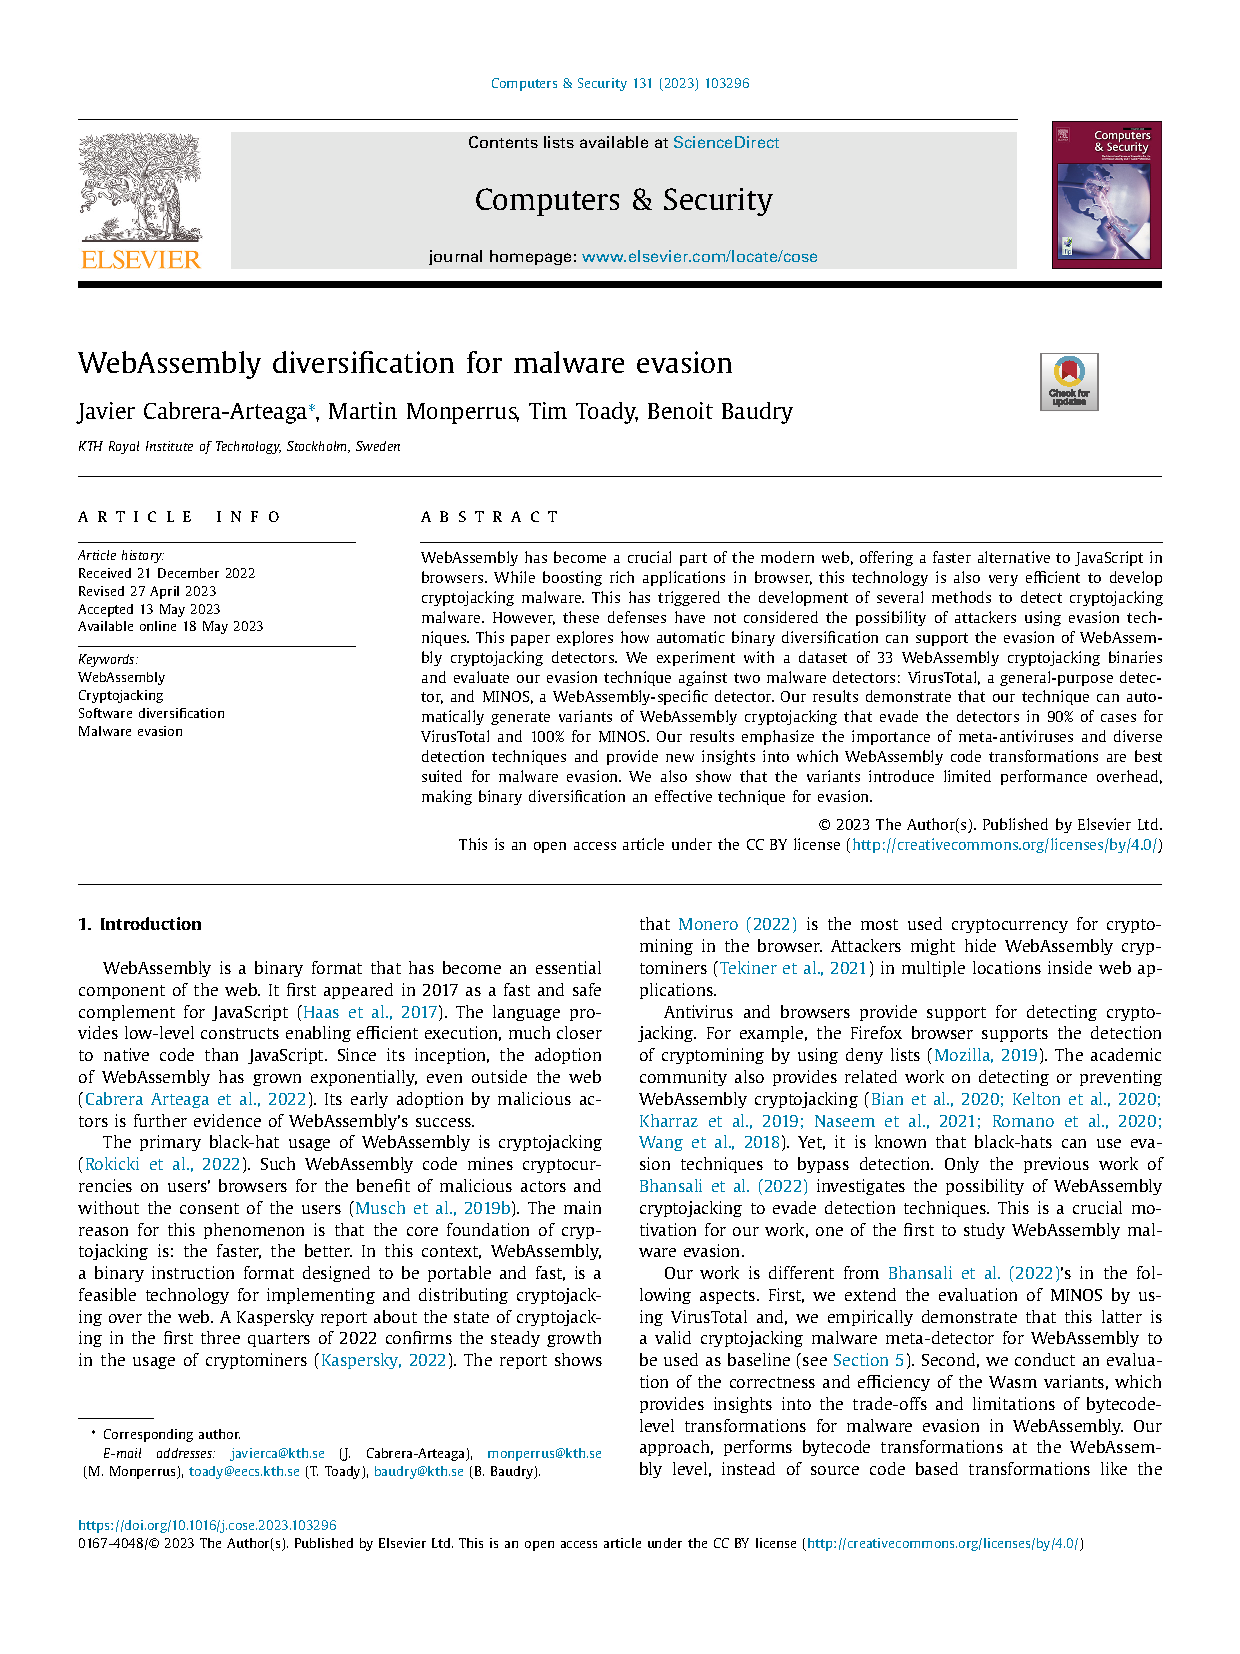
\includepdf[pages=1-16]{papers/evasion.pdf}} % 
    {} %
    

\chapter{\mbox{WASM-MUTATE}:~Fast~and~Effective~Binary~Diversification~for~\mbox{WebAssembly}}
\textbf{Javier Cabrera-Arteaga}, Nick Fitzgerald, Martin Monperrus, Benoit Baudry\\
\emph{Computers \& Security, 2024}\\\\
\url{https://www.sciencedirect.com/science/article/pii/S0167404824000324}\\\\

\ifthenelse{\equal{\ADDCONTRIB}{True}}%
    {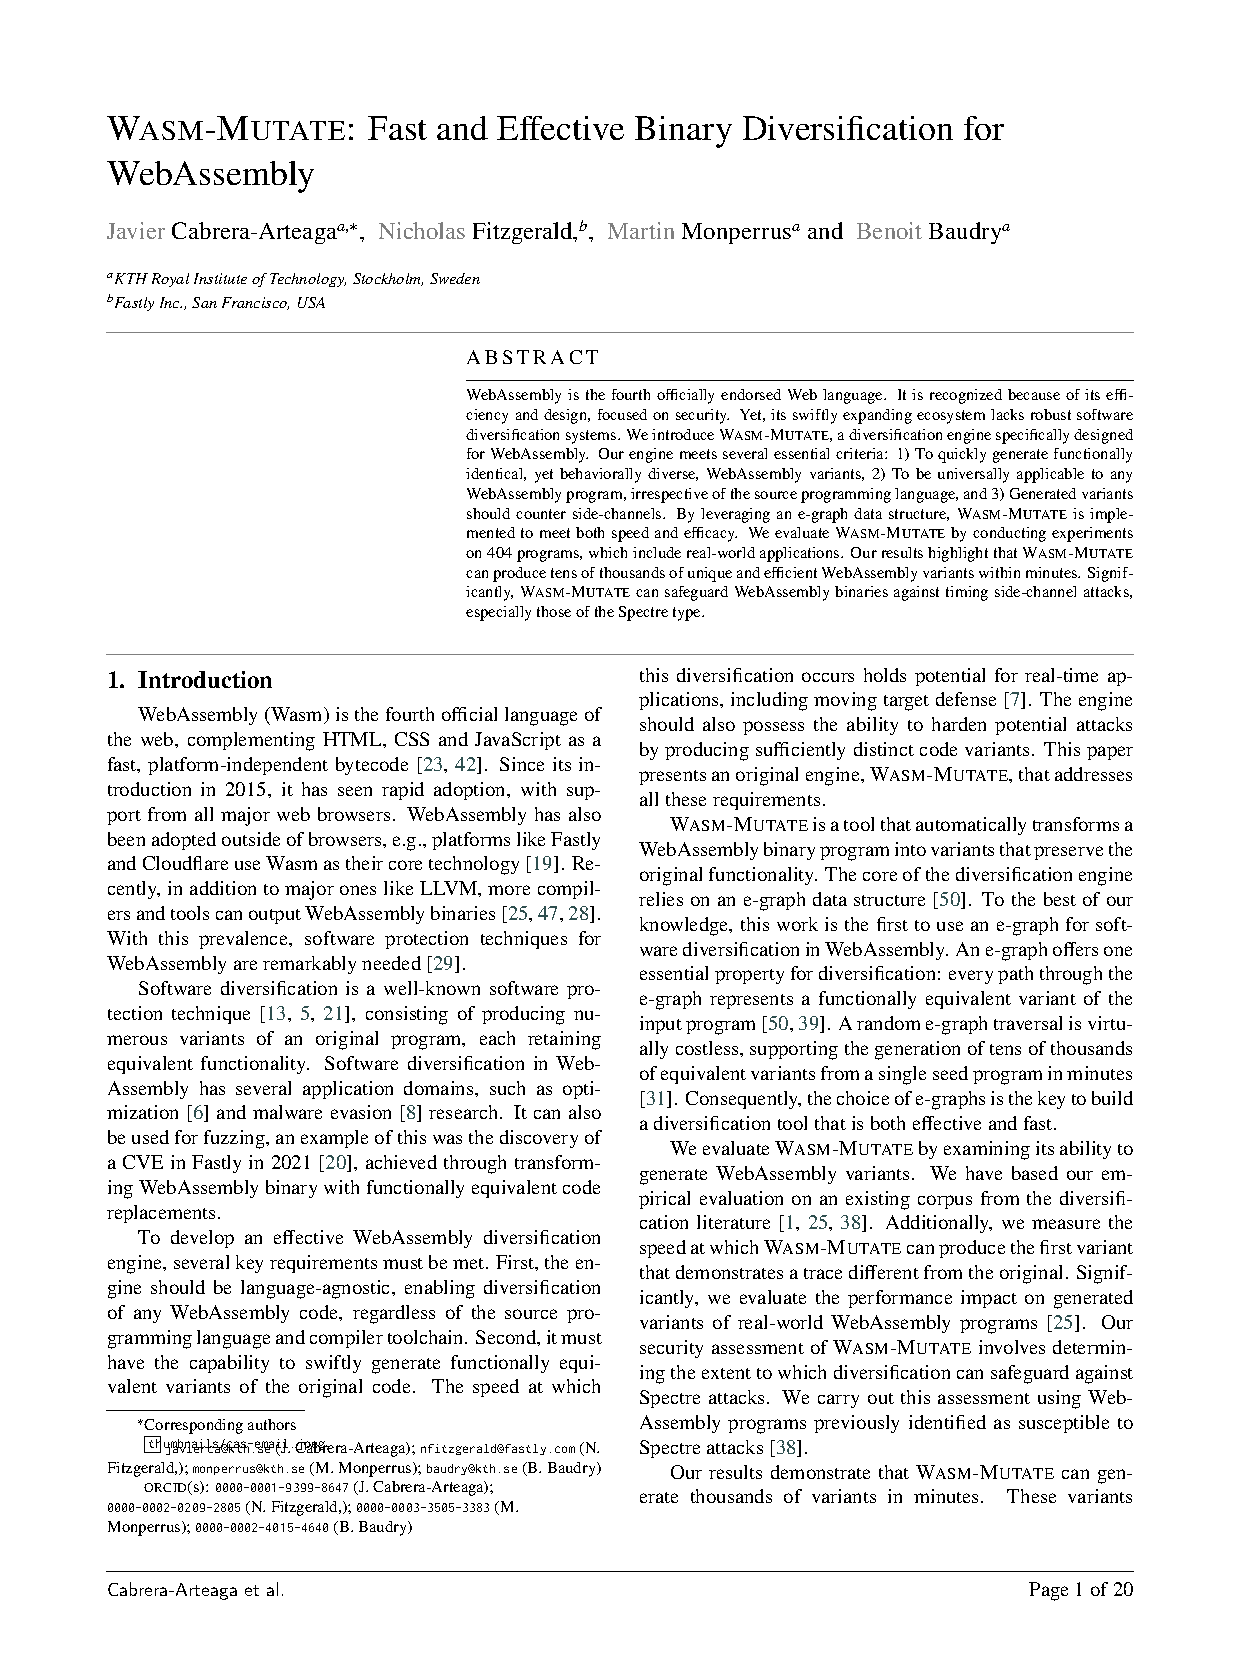
\includepdf[pages=1-20]{papers/wasm-mutate-v2.pdf}} % 
    {} %


% Add paper here
\chapter{CROW: Code Diversification for WebAssembly}

\textbf{Javier Cabrera-Arteaga}, Orestis Floros, Oscar Vera-Pérez, Benoit Baudry, Martin Monperrus\\
\emph{Network and Distributed System Security Symposium (NDSS 2021), Workshop on Measurements, Attacks, and Defenses for the Web}\\\\
\url{https://doi.org/10.14722/madweb.2021.23004}\\

\ifthenelse{\equal{\ADDCONTRIB}{True}}%
    {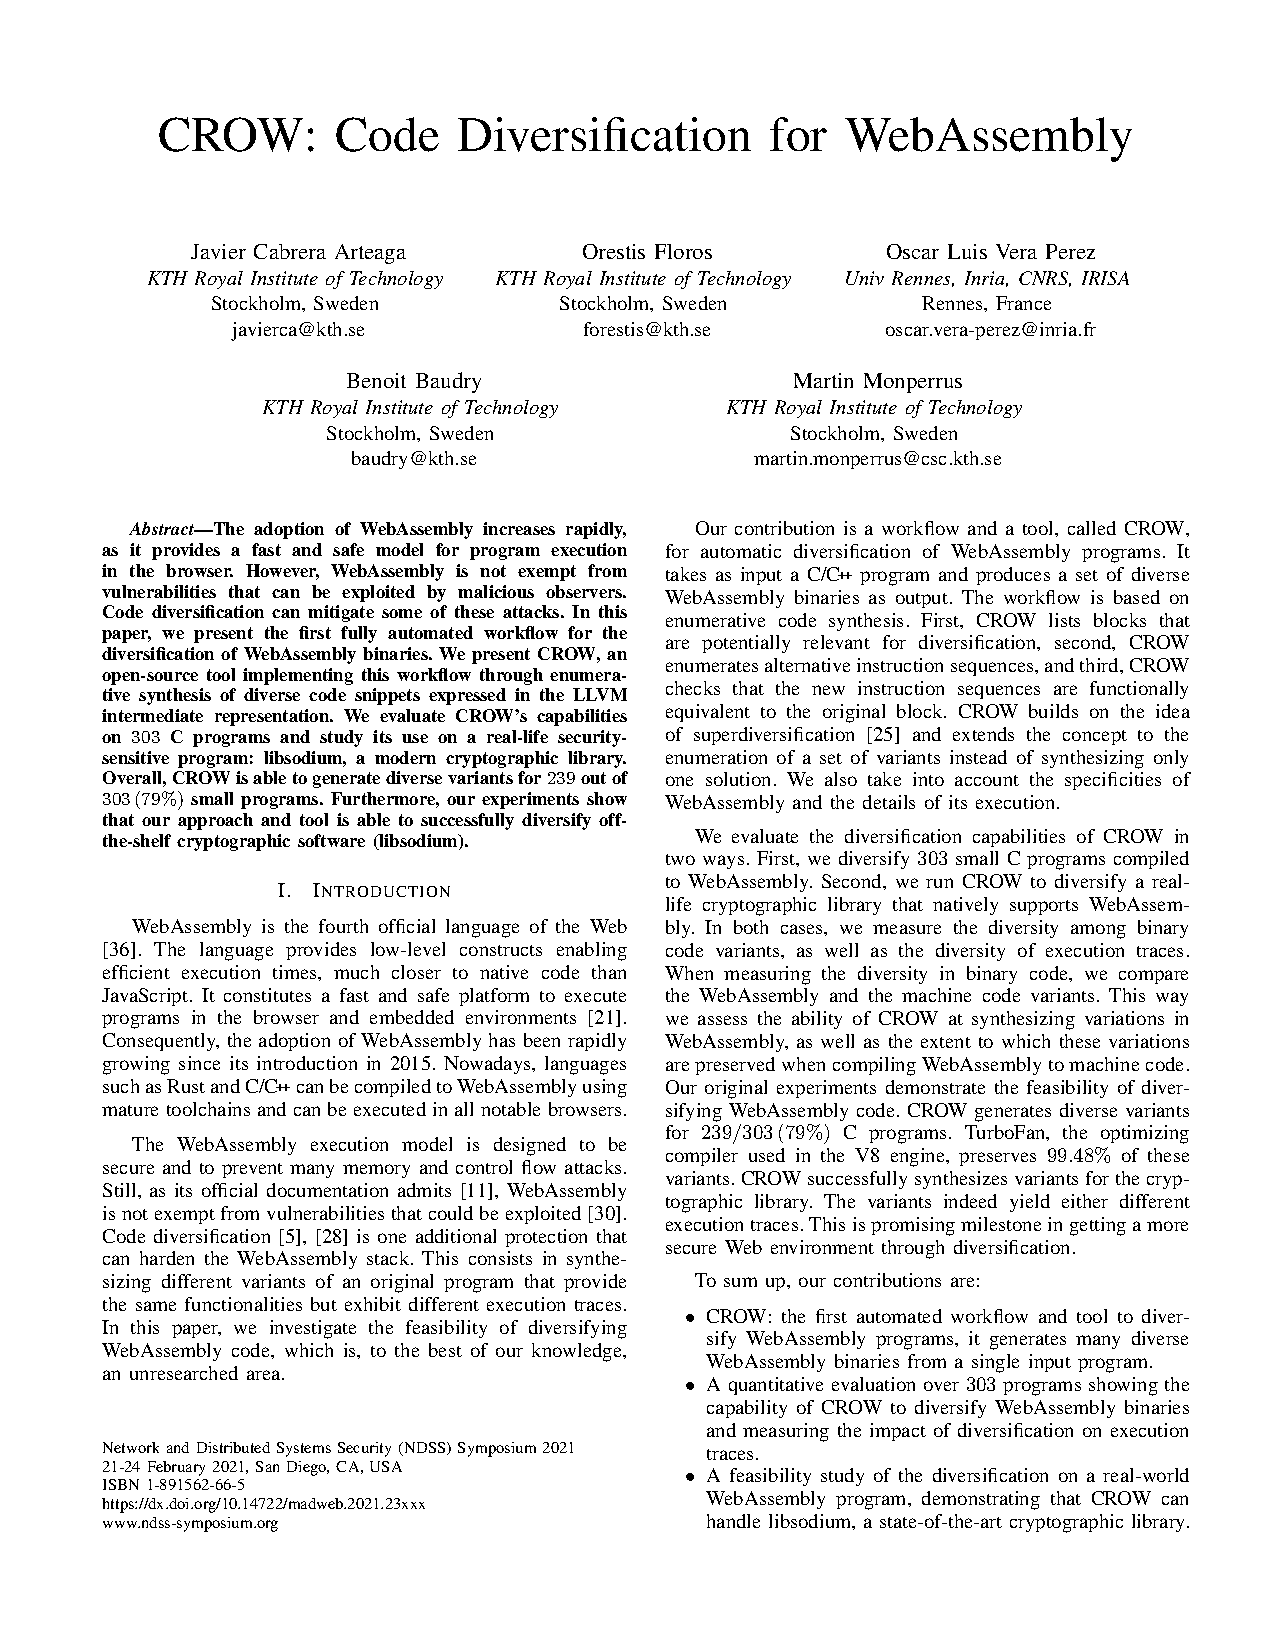
\includepdf[pages=1-12]{papers/crow.pdf}} %
    {} % 
    
\chapter{Multi-Variant Execution at the Edge}

\textbf{Javier Cabrera-Arteaga}, Pierre Laperdrix, Martin Monperrus, Benoit Baudry\\
\emph{Conference on Computer and Communications Security (CCS 2022), Workshop on Moving Target Defense (MTD)}\\\\
 \url{https://dl.acm.org/doi/abs/10.1145/3560828.3564007}\\\\

\ifthenelse{\equal{\ADDCONTRIB}{True}}%
    {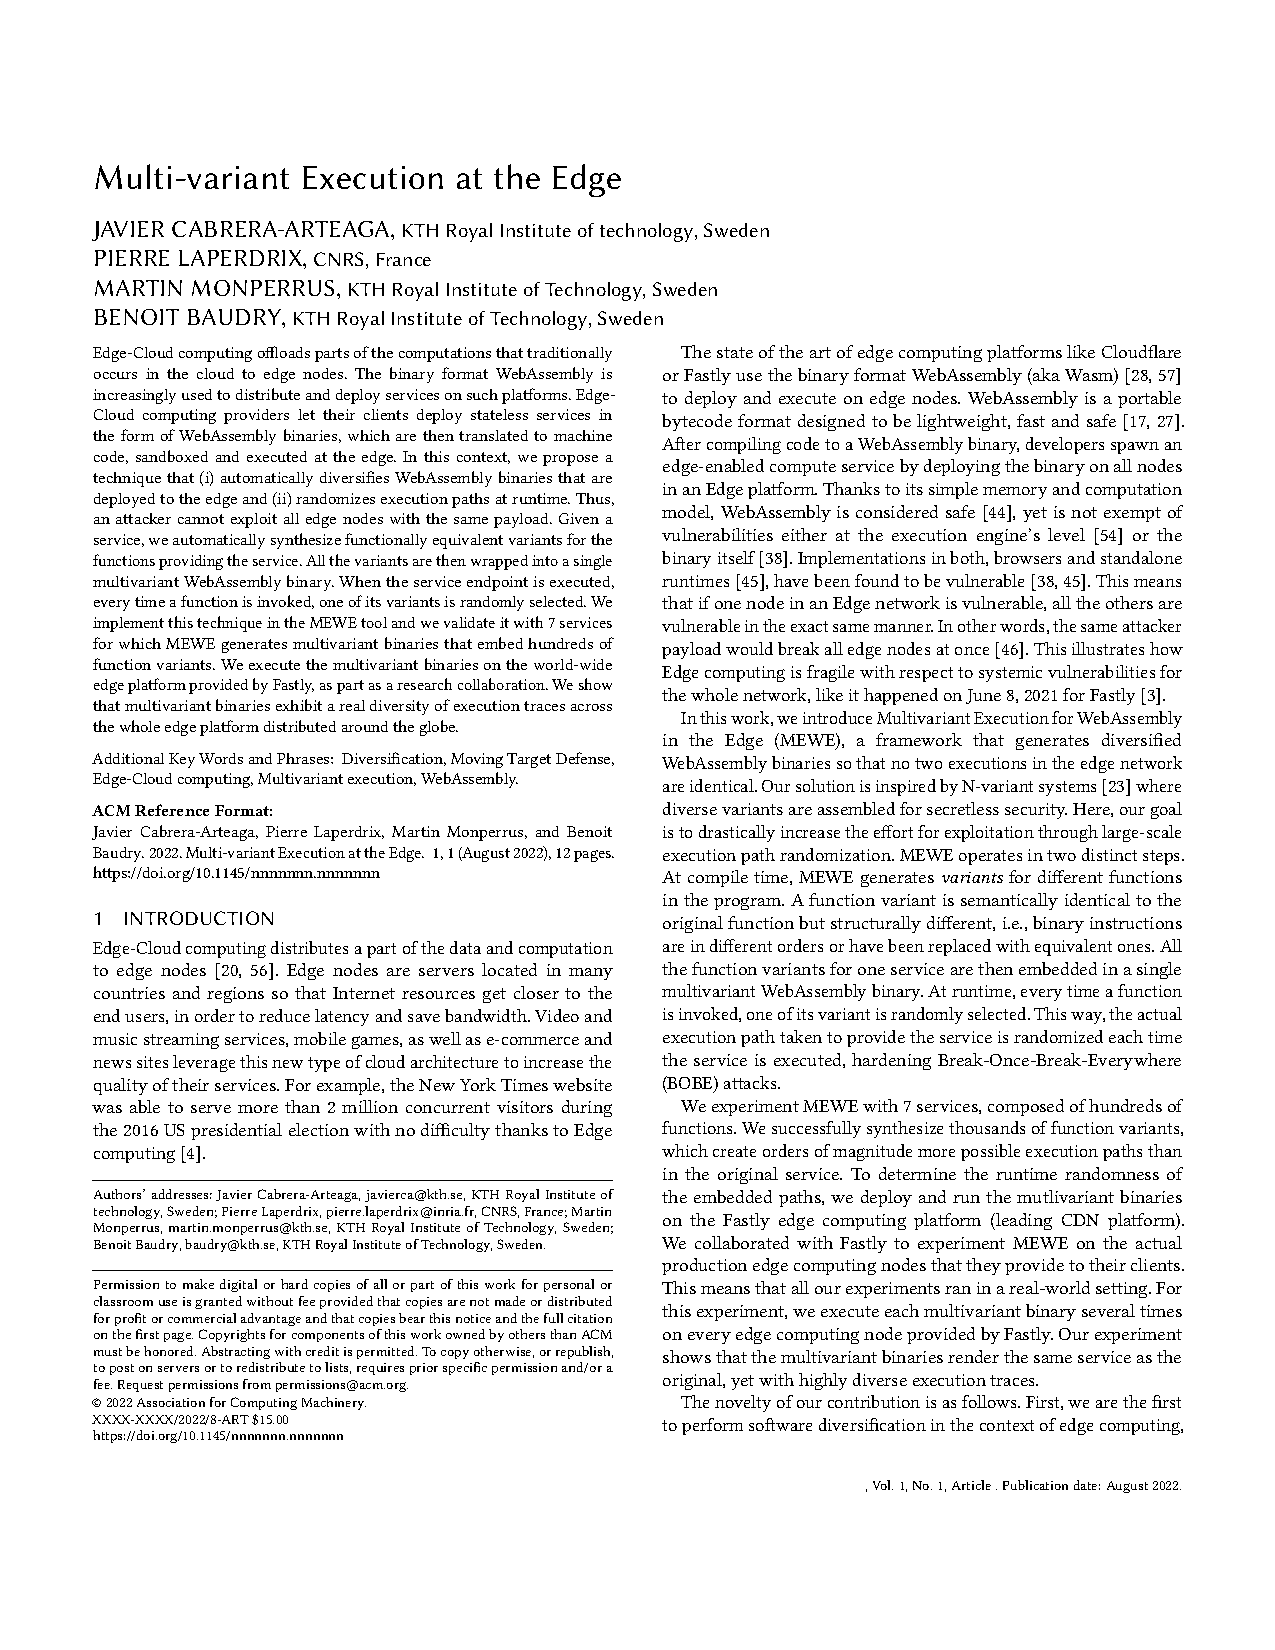
\includepdf[pages=1-12]{papers/mewe_final.pdf}} % 
    {} %
    
  \chapter{Superoptimization of WebAssembly Bytecode}

  \textbf{Javier Cabrera-Arteaga}, Shrinish Donde, Jian Gu, Orestis Floros, Lucas Satabin, Benoit Baudry, Martin Monperrus\\
  \emph{Conference Companion of the 4th International Conference on Art, Science, and Engineering of Programming (Programming 2021), MoreVMs}\\\\
  \url{https://doi.org/10.1145/3397537.3397567}\\
  
  % Add Abstract
  
  \ifthenelse{\equal{\ADDCONTRIB}{True}}%
      {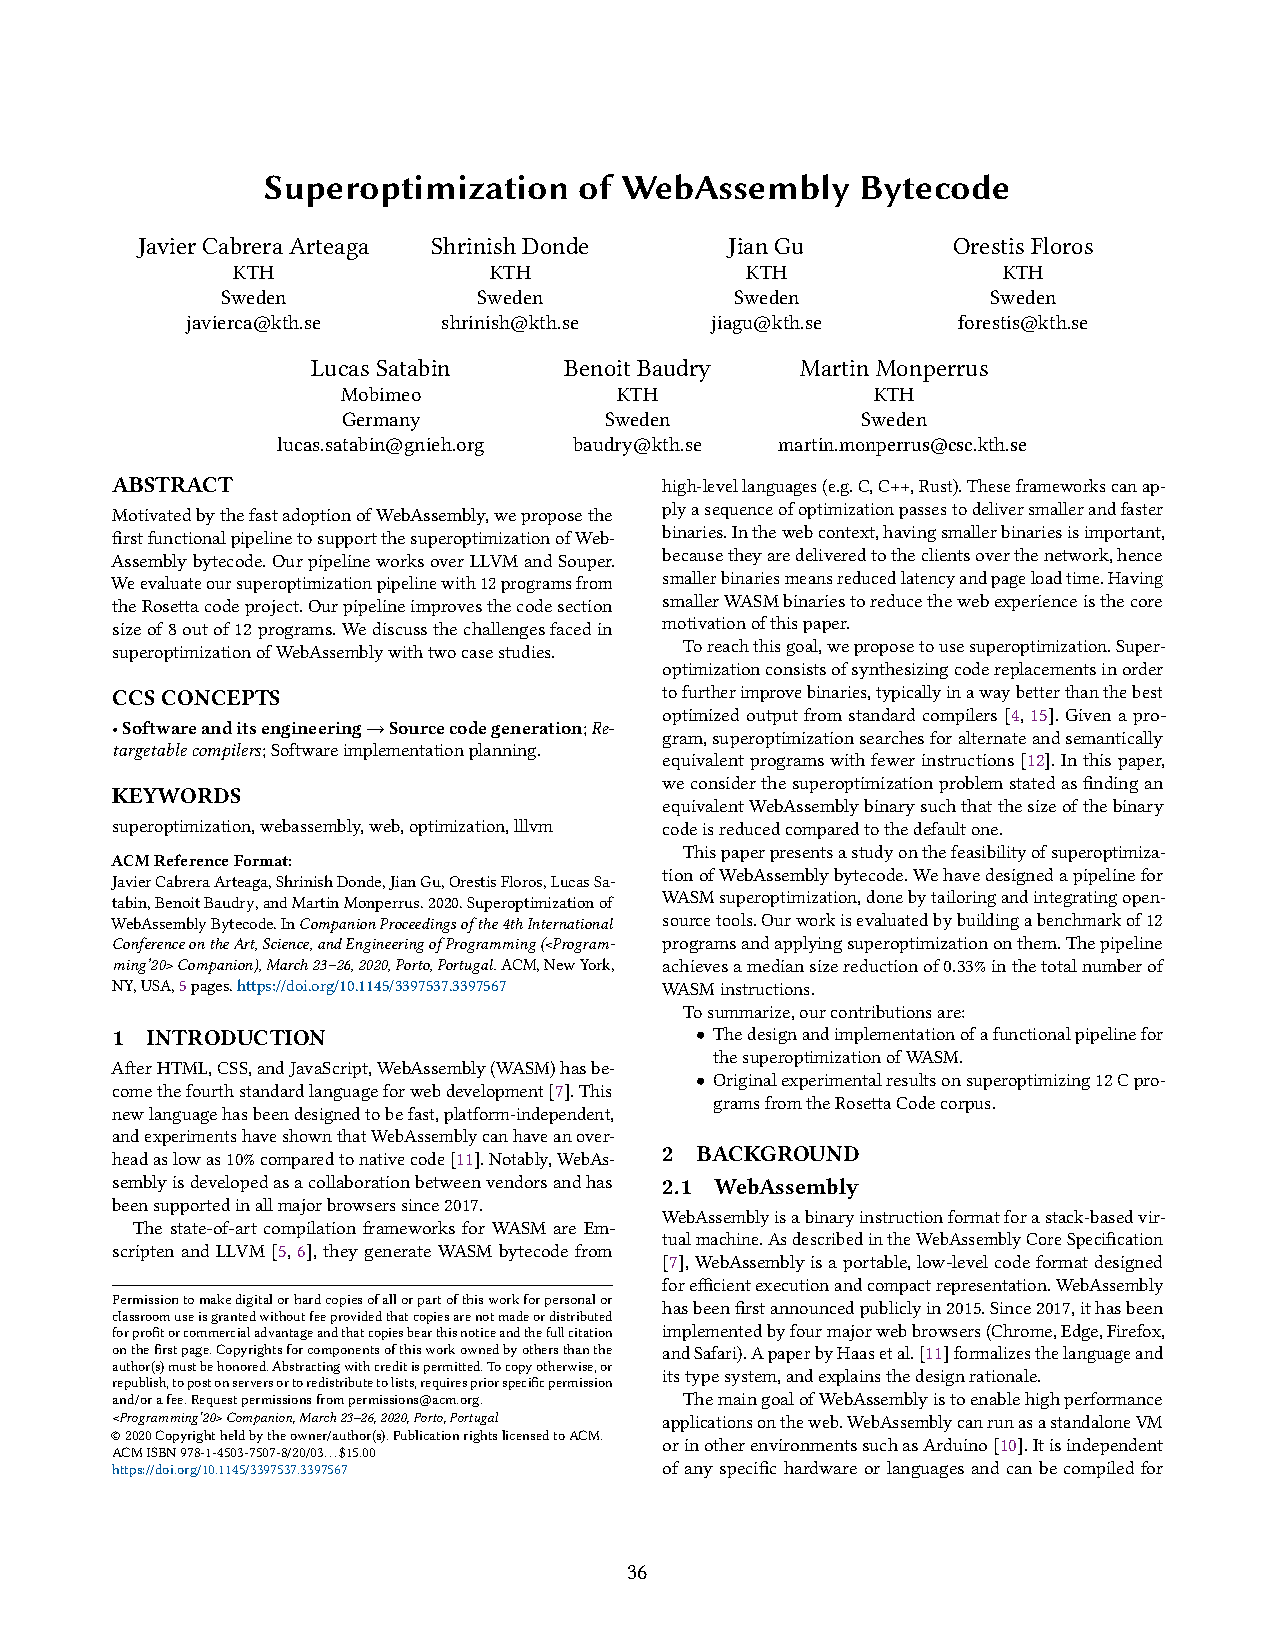
\includepdf[pages=1-5]{papers/souper.pdf}} % 
      {} %
    
\chapter{Scalable Comparison of JavaScript V8 Bytecode Traces}

\textbf{Javier Cabrera-Arteaga}, Martin Monperrus, Benoit Baudry\\
\emph{11th ACM SIGPLAN International Workshop on Virtual Machines and Intermediate Languages (SPLASH 2019)}\\\\
\url{https://doi.org/10.1145/3358504.3361228}\\


\ifthenelse{\equal{\ADDCONTRIB}{True}}%
    {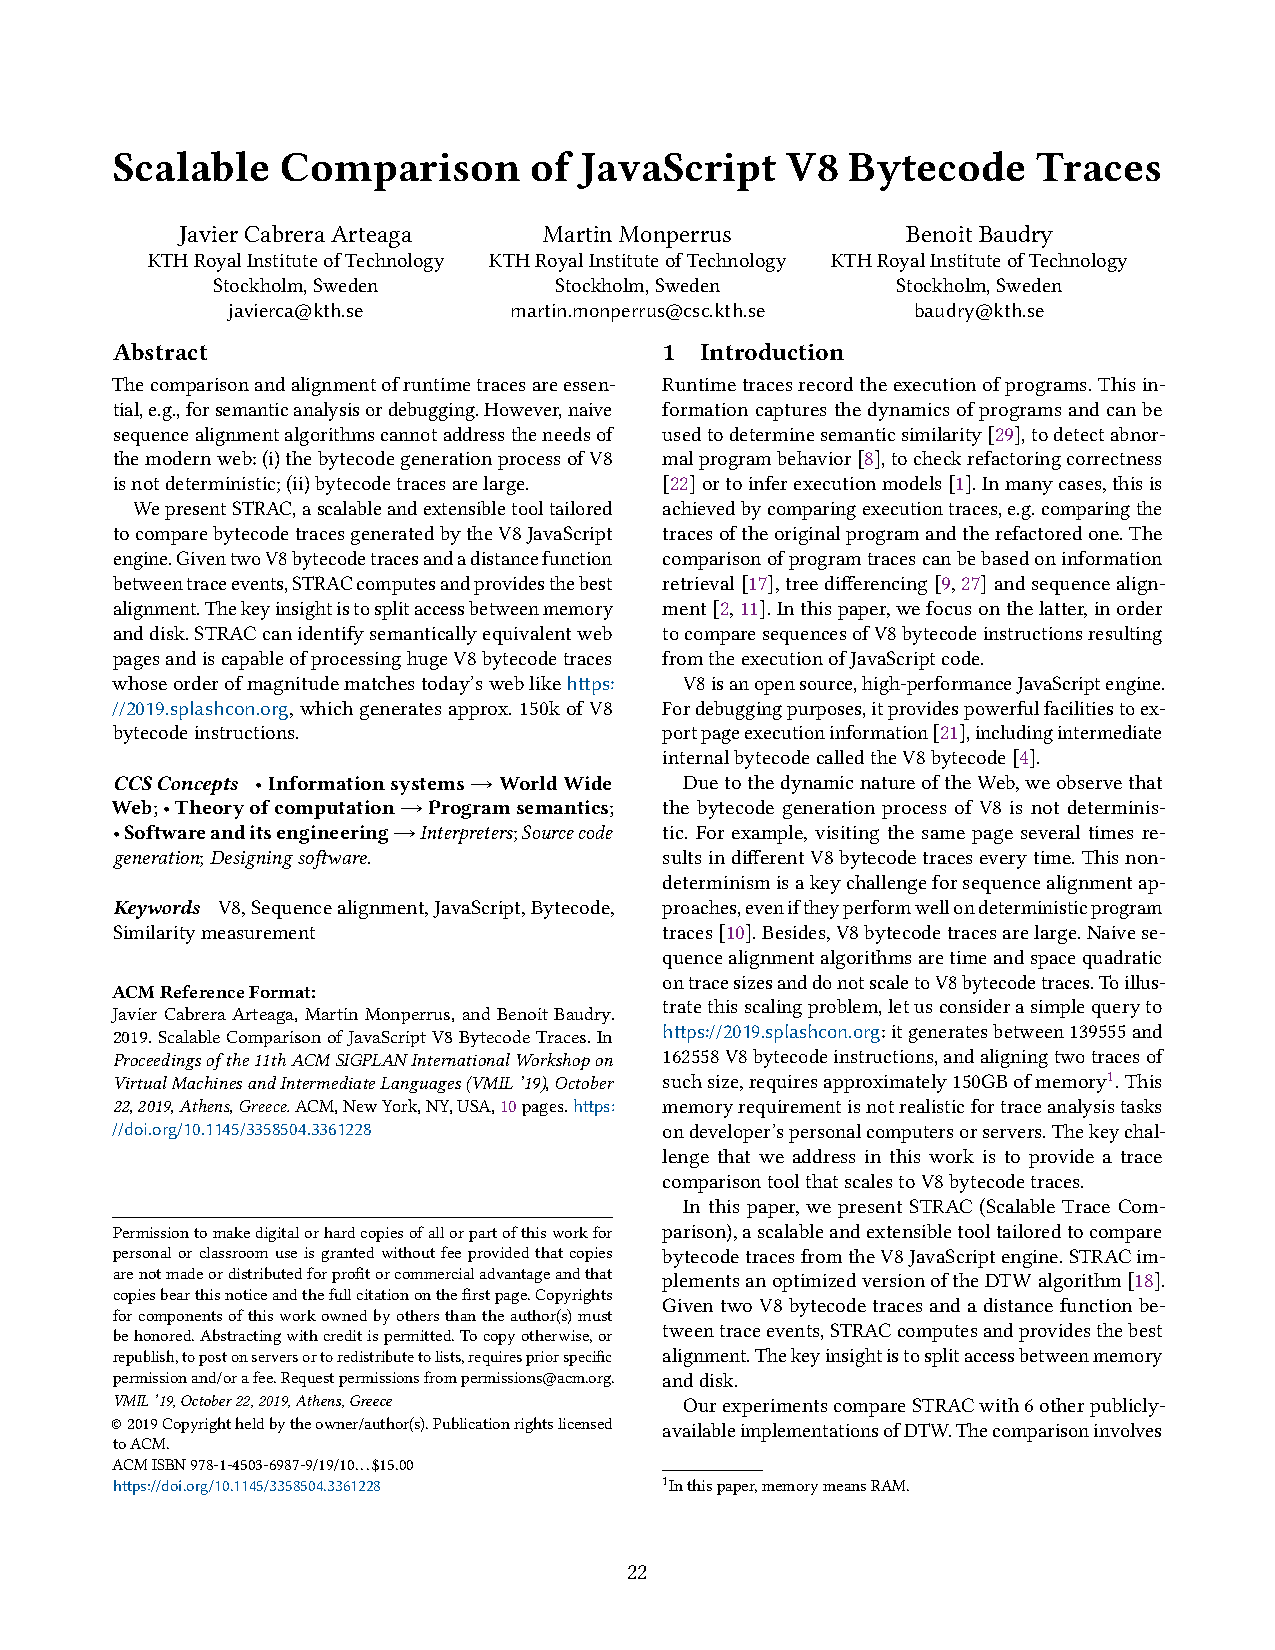
\includepdf[pages=1-10]{papers/STRAC.pdf}} %
    {} %
    
\printindex

\end{document}
\endinput
%%
%% End of file `kth-demo.tex'.
